\pagestyle{chu}
\newwatermark[pagex={4}]{\vspace{2.5cm}\hspace*{7.8cm}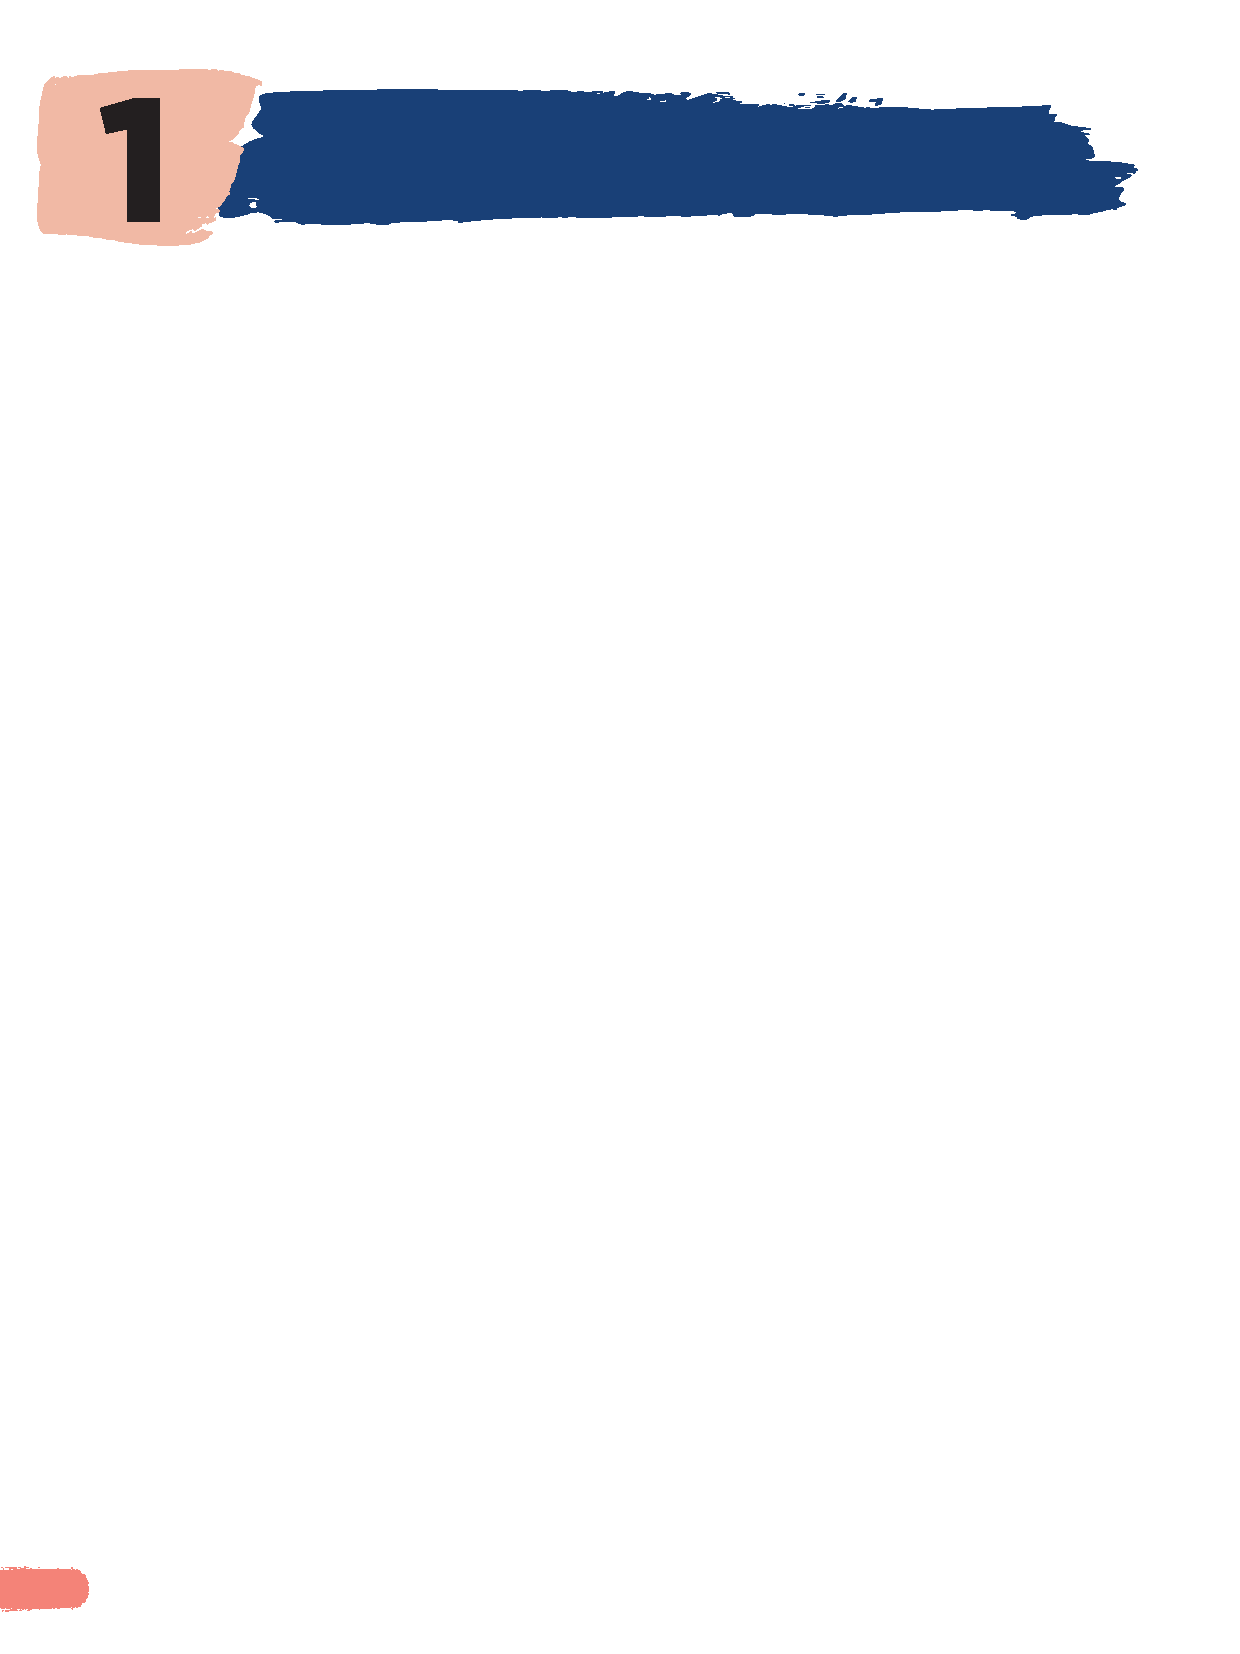
\includegraphics[scale=1]{../watermarks/1modulo5ano.pdf}}
\newwatermark[pagex={12}]{\vspace{2.5cm}\hspace*{7.8cm}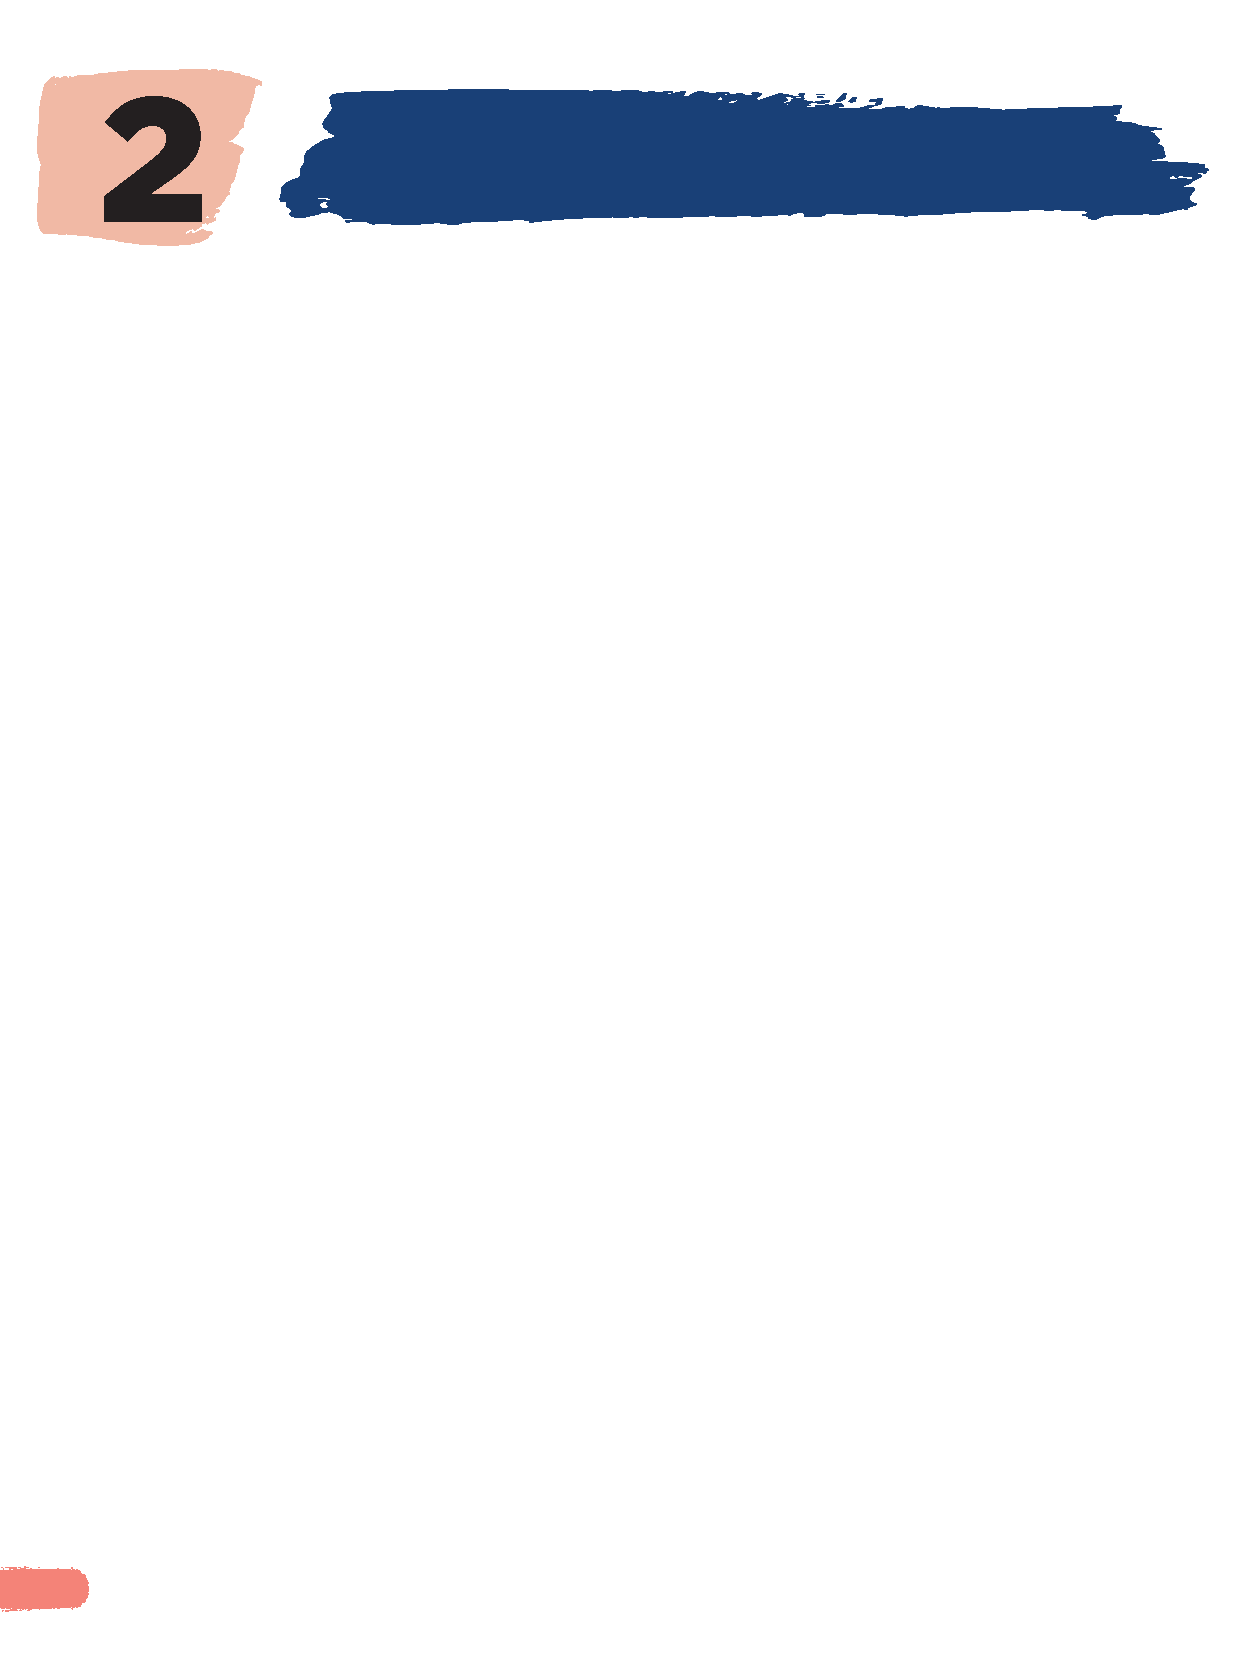
\includegraphics[scale=1]{../watermarks/2modulo5ano.pdf}}
\newwatermark[pagex={20}]{\vspace{2.5cm}\hspace*{7.8cm}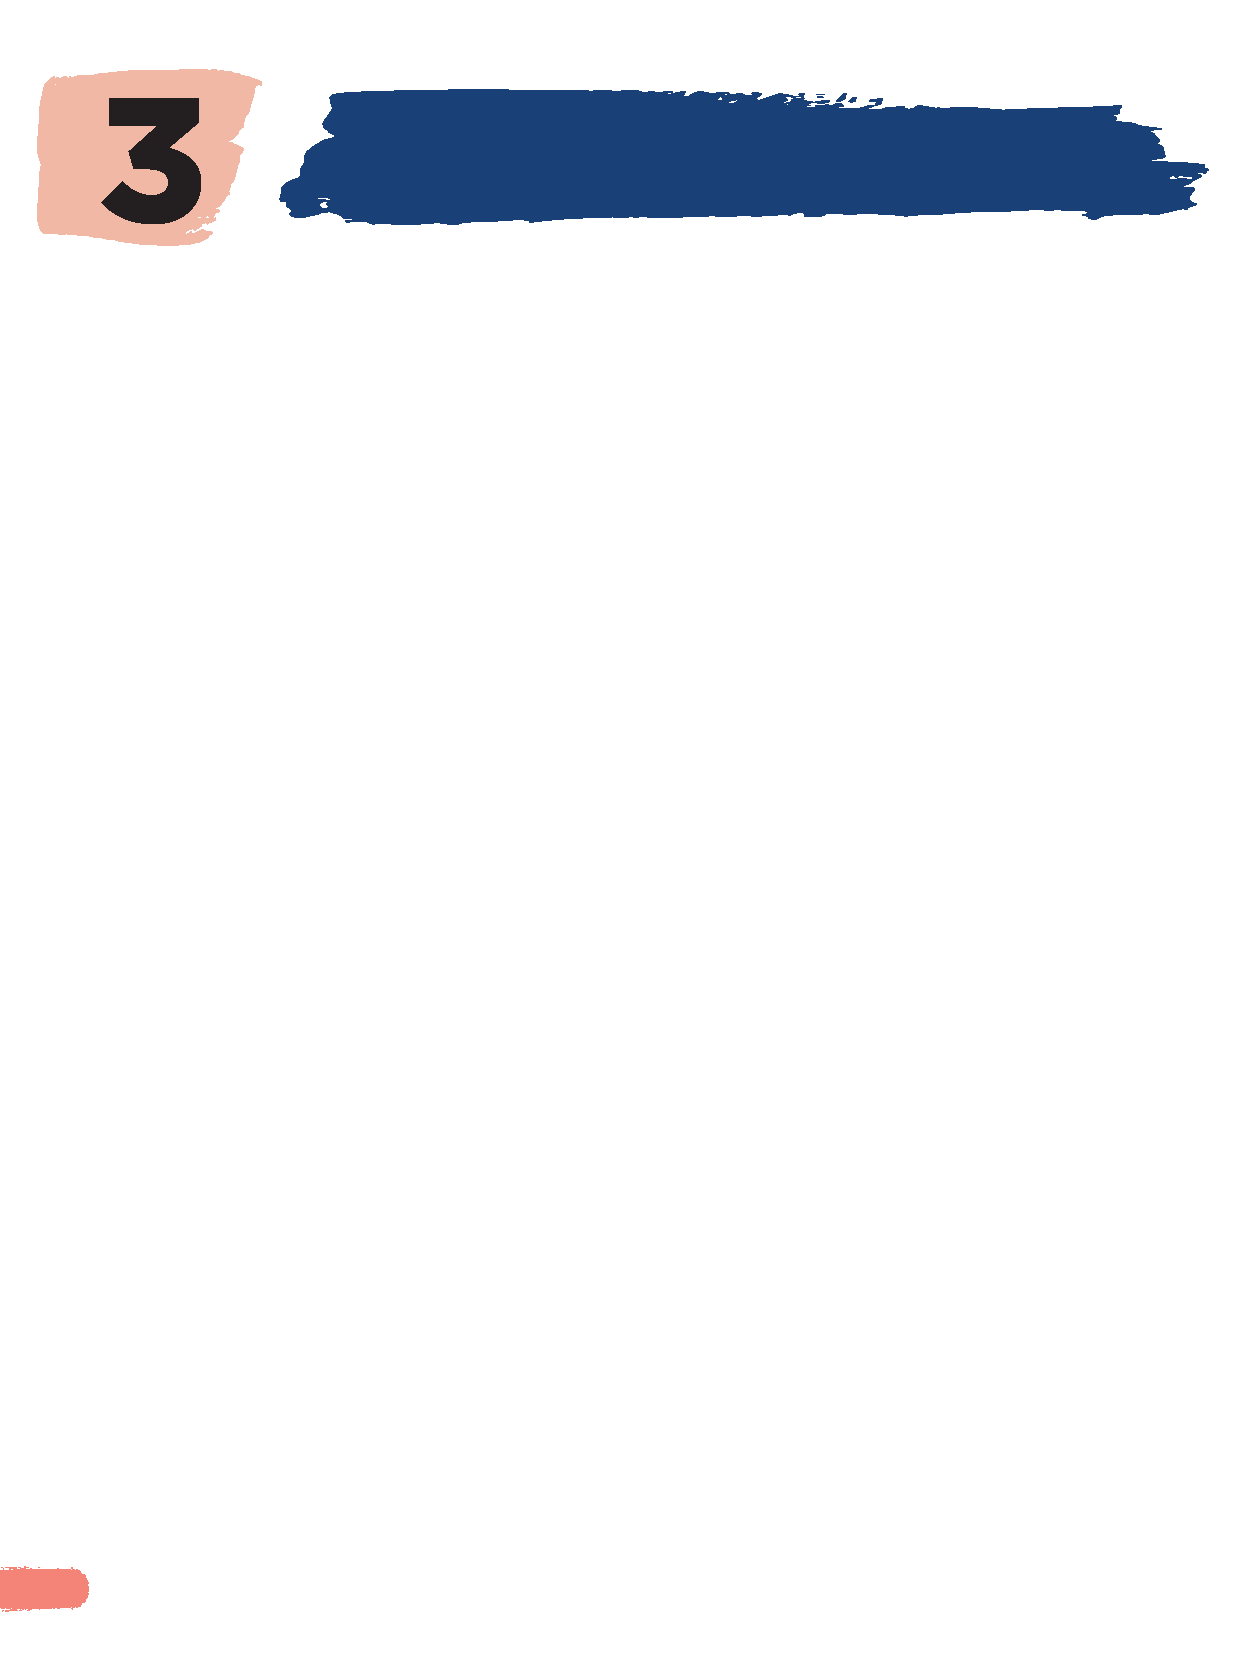
\includegraphics[scale=1]{../watermarks/3modulo5ano.pdf}}
\newwatermark[pagex={29}]{\vspace{2.5cm}\hspace*{7.8cm}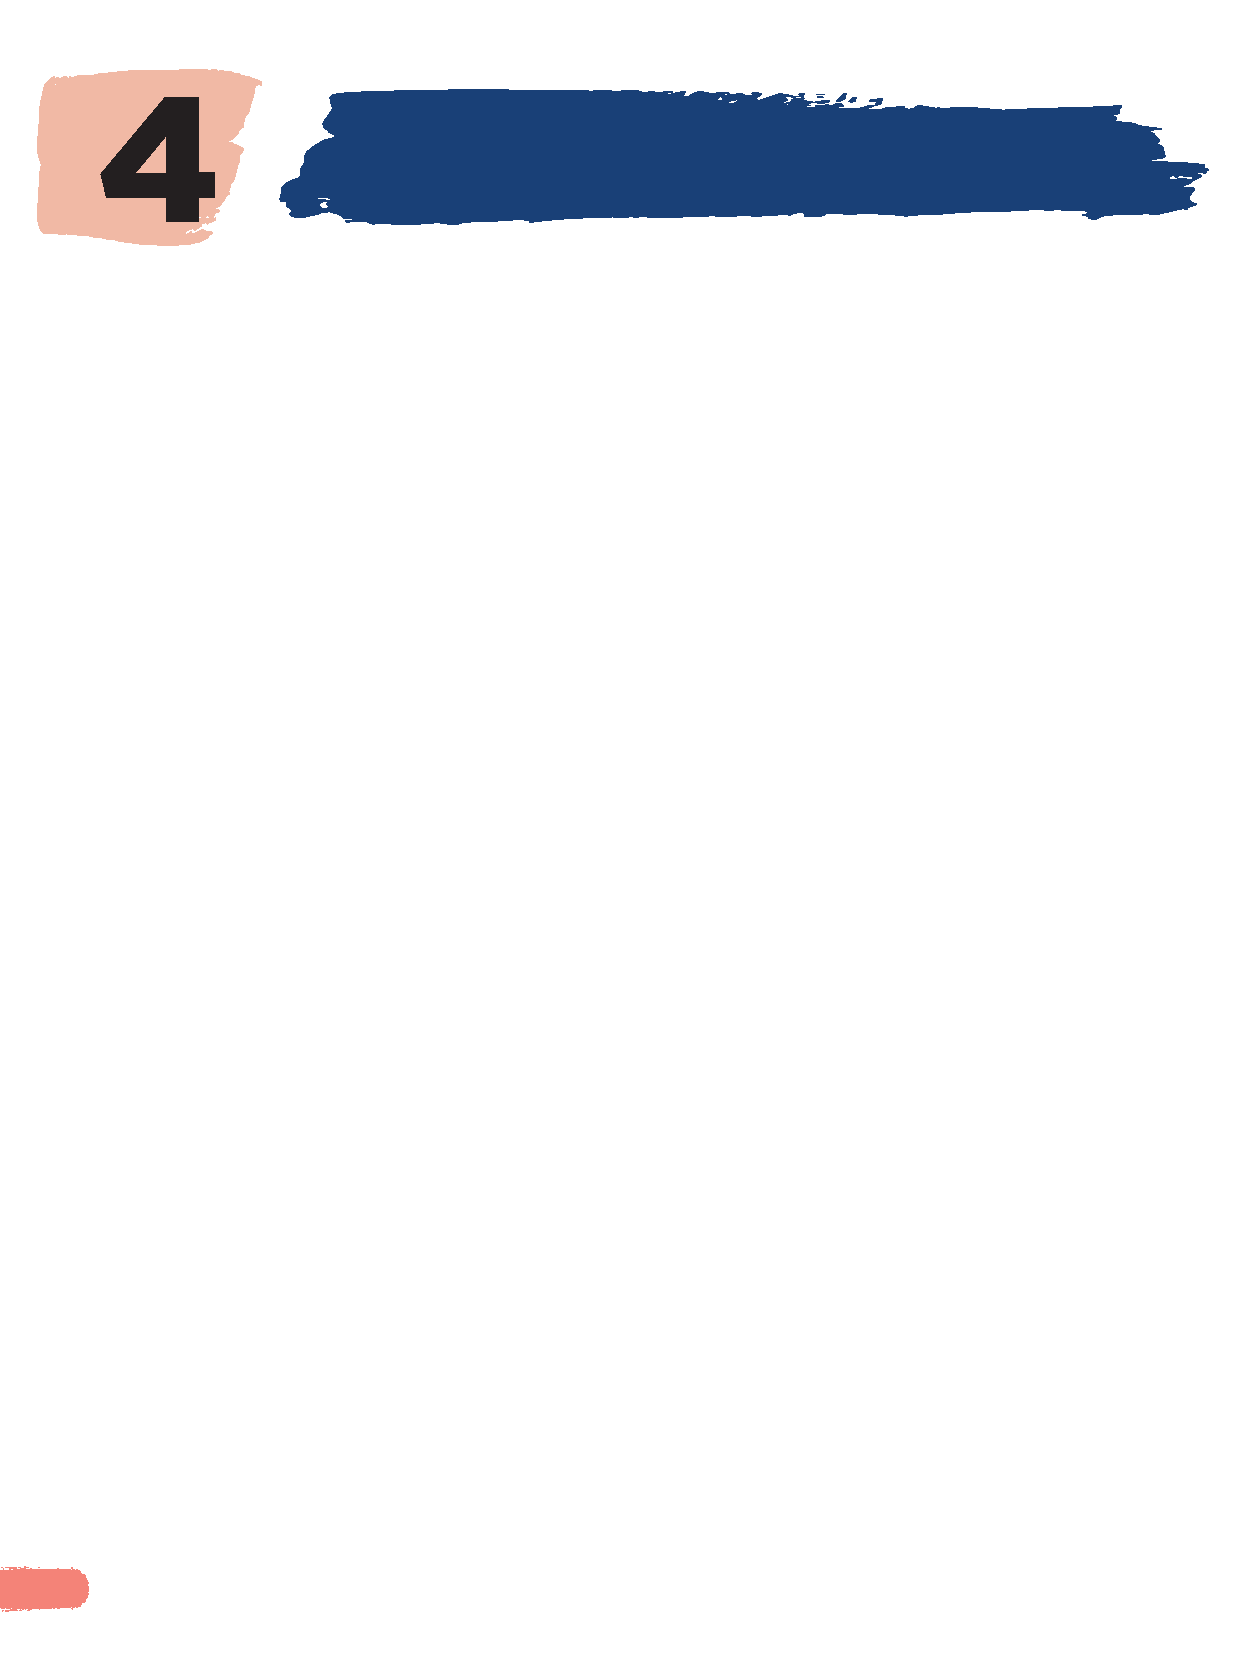
\includegraphics[scale=1]{../watermarks/4modulo5ano.pdf}}
\newwatermark[pagex={38}]{\vspace{2.5cm}\hspace*{7.8cm}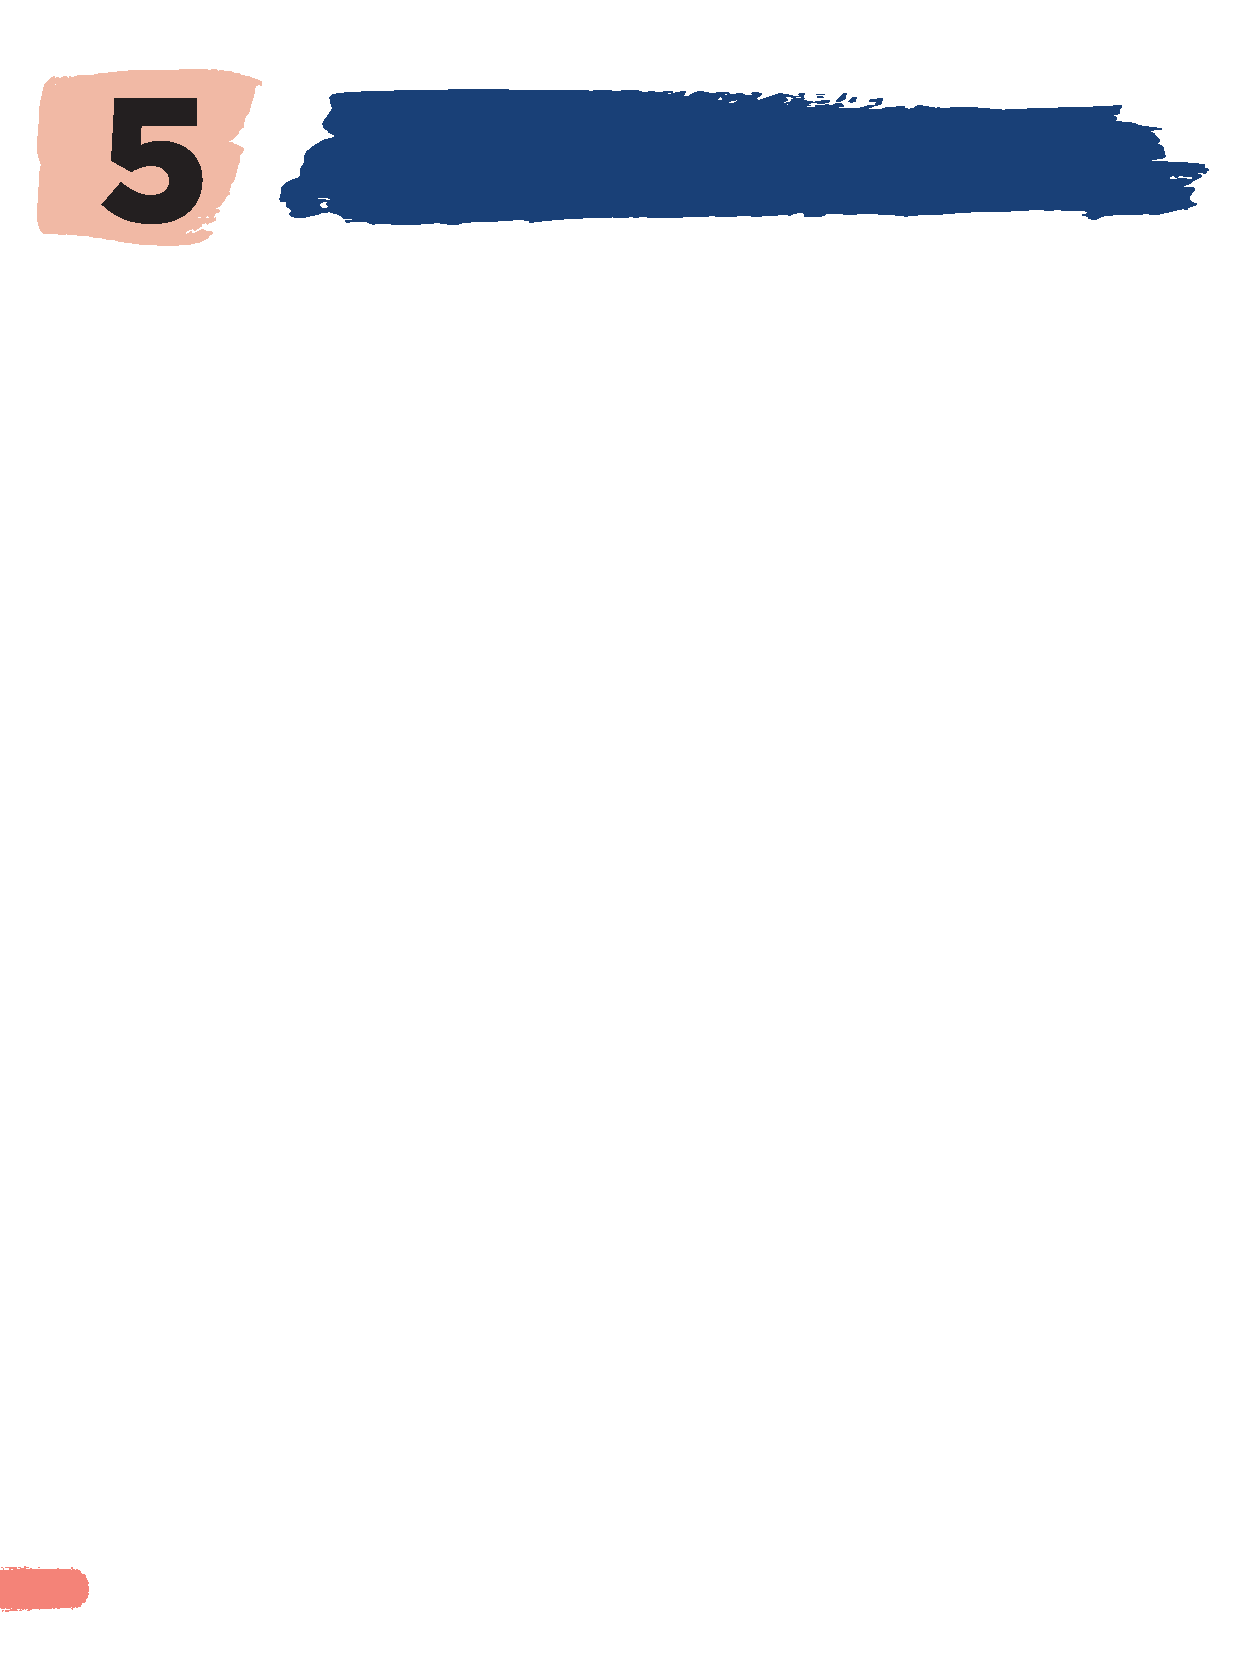
\includegraphics[scale=1]{../watermarks/5modulo5ano.pdf}}
\newwatermark[pagex={47}]{\vspace{2.5cm}\hspace*{7.8cm}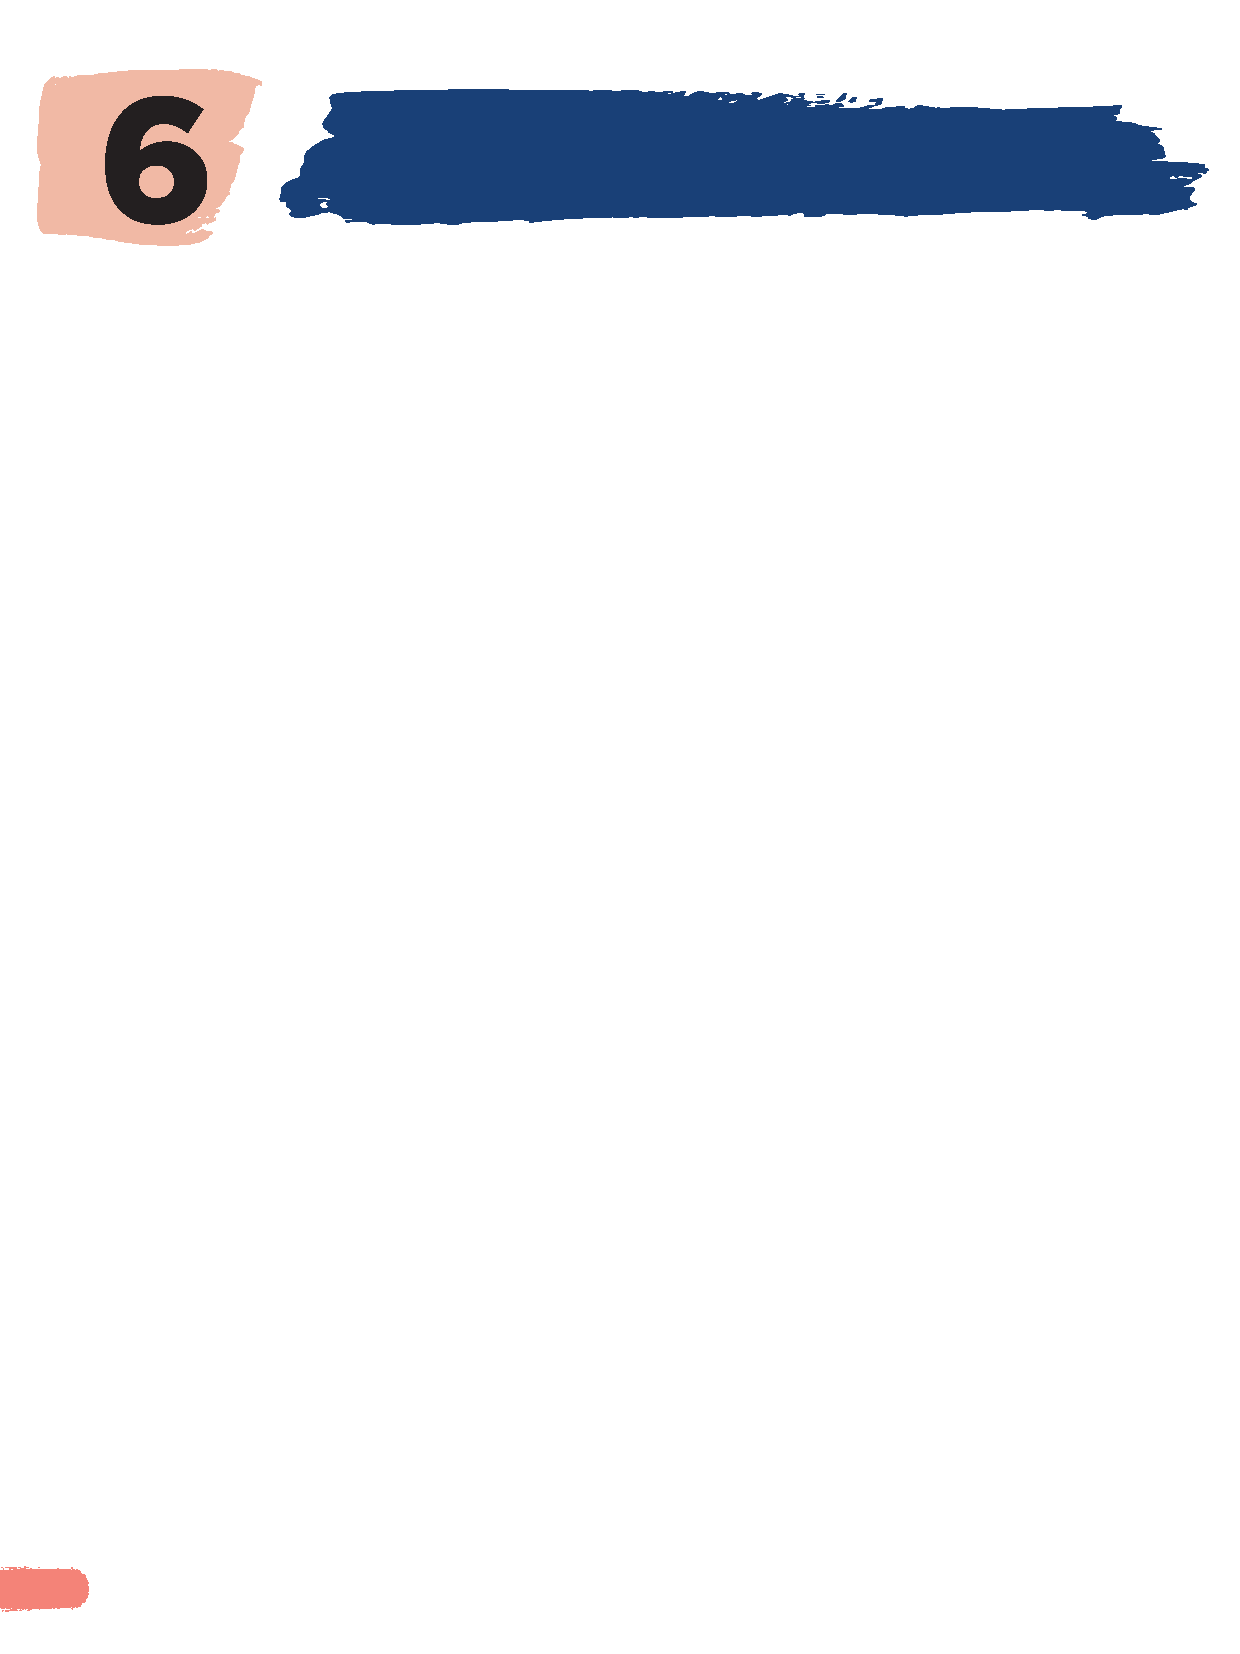
\includegraphics[scale=1]{../watermarks/6modulo5ano.pdf}}
\newwatermark[pagex={5,7,9,11,13,15,17,19,21,23,25,27,31,33,35,37,39,41,43,45,49,51,53,55}]{\vspace{2.5cm}\hspace*{8cm}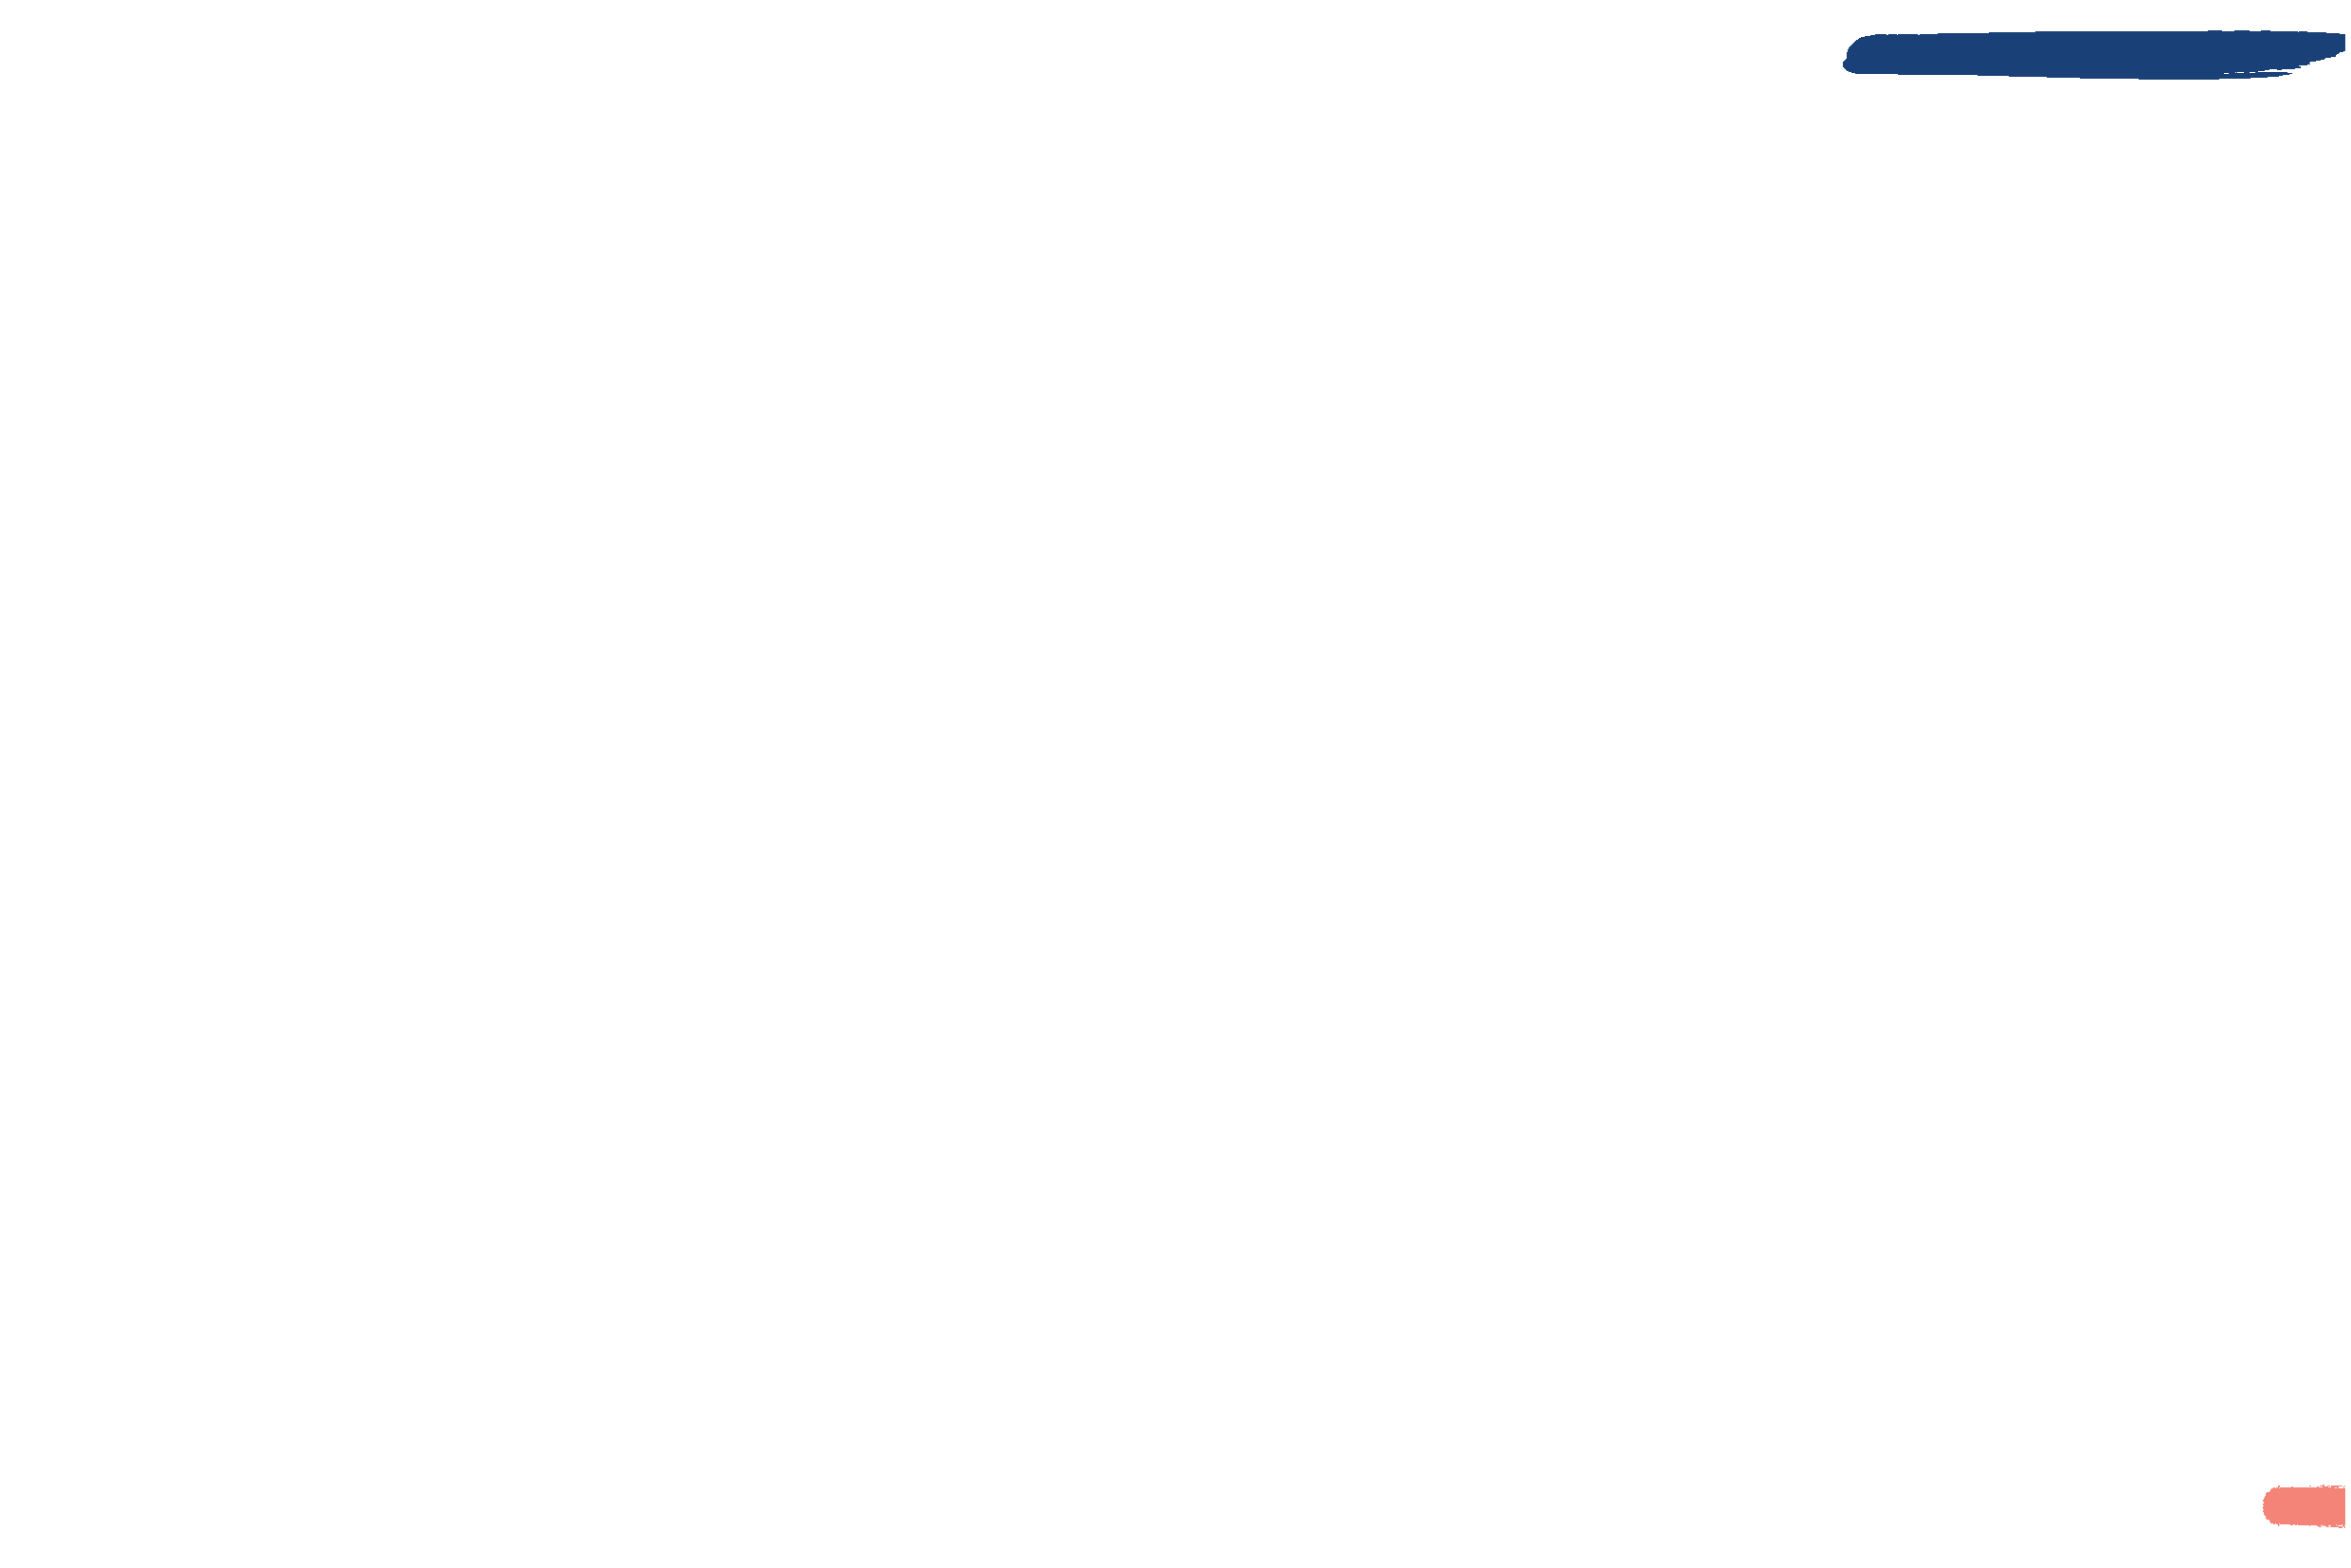
\includegraphics[scale=1]{../watermarks/bg5anoimpar.pdf}}
\newwatermark[pagex={6,8,10,14,16,18,20,22,24,26,28,30,32,34,36,40,42,44,46,48,50,52,54}]{\vspace{2.5cm}\hspace*{7.8cm}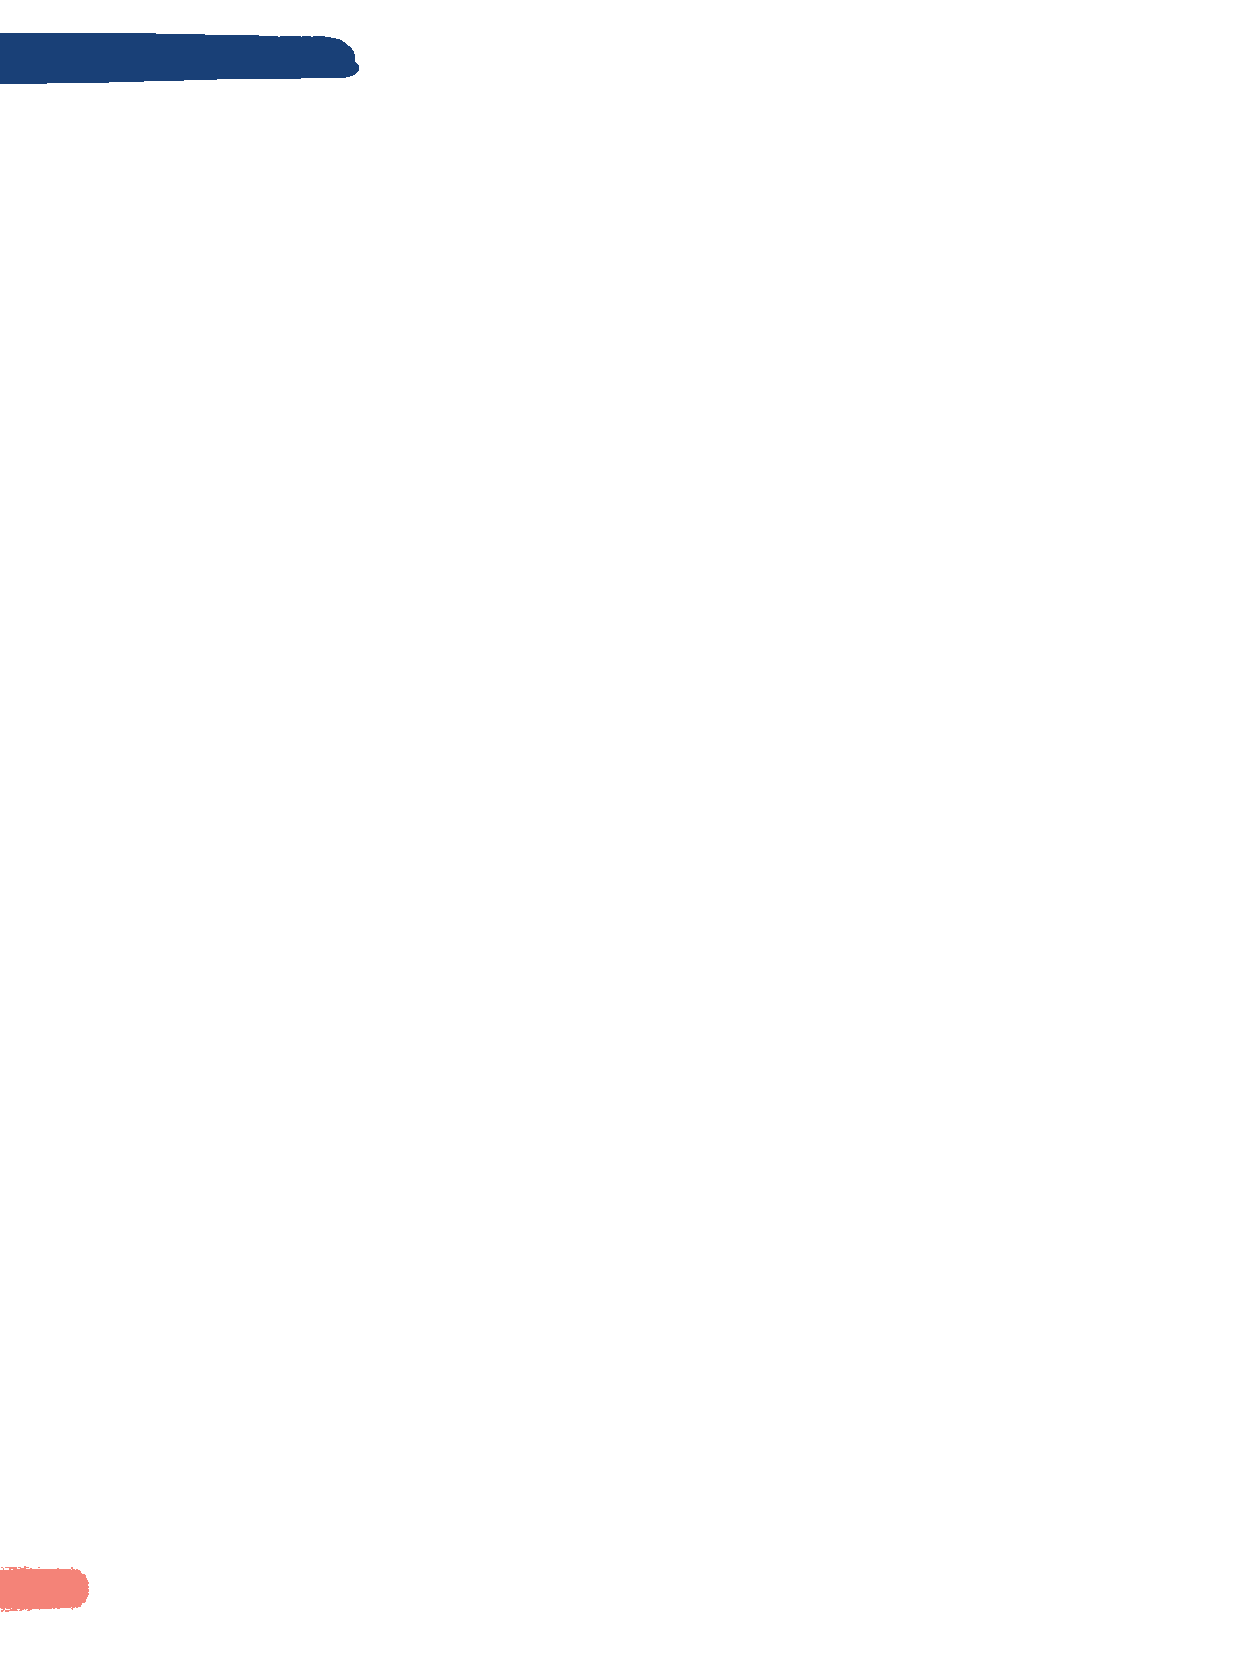
\includegraphics[scale=1]{../watermarks/bg5anopar.pdf}}

\chapter[Representações de tempo e espaço]{\LARGE Representações de tempo e espaço}
\markboth{Módulo 1}{}

%Orientações para o professor:

\coment{Habilidades da BNCC: EF05HI01, EF05HI07, EF05HI08.}

\colorsec{Eixo de conhecimento do SAEB}

\begin{itemize}
\item Tempo e espaço: fontes e formas de representação.
\end{itemize}

%{\emph{https://br.freepik.com/vetores-gratis/o-tempo-voa-ilustracao-do-conceito\_28771041.htm\#page=2\&query=tempo\&position=38\&from\_view=search\&track=sph}}
%Acesso em: 23 fev. 2023

\conteudo{O que o tempo influencia em quem somos, em como vivemos e em onde vivemos?
Você já parou para pensar que temos tempo para tudo? Tempo de acordar,
tempo de ir para a escola, tempo de comer, tempo de dormir etc.? Também
nos medimos pelo tempo: contamos quanto tempo passou desde que nascemos
e chamamos isso de idade. Mudamos com o tempo. De pequenos, vamos
crescendo. Com o tempo aprendemos coisas novas, construímos prédios,
pontes e relações de afeto. Nossa vida, assim como o mundo, gira em
torno do tempo.

\begin{wrapfigure}{l}{.3\textwidth}
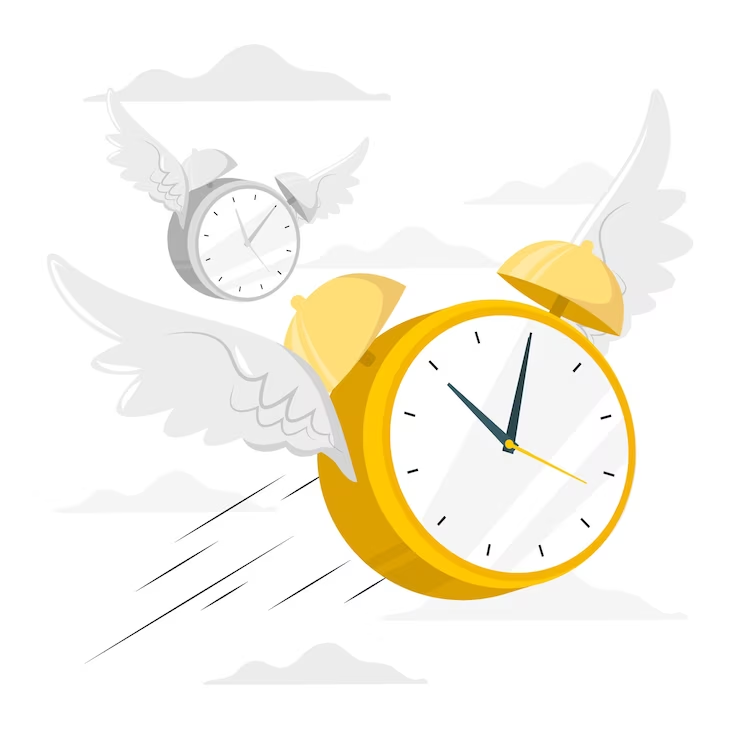
\includegraphics[width=.35\textwidth]{./imgs/img26.png}
\end{wrapfigure}

Há milhões de anos, os humanos não existiam. Com o tempo,
microrganismos que existiam no planeta Terra deram origem a milhares de
espécies até chegarem a nós. Com o tempo, de seres individuais que
buscavam somente o próprio alimento, passamos a nos unir. Demos início à
nossa história, à história da humanidade. Formamos comunidades, que
viraram povos, que construíram cidades. Ocupamos o mundo e trabalhamos
muito tempo para chegar até aqui.


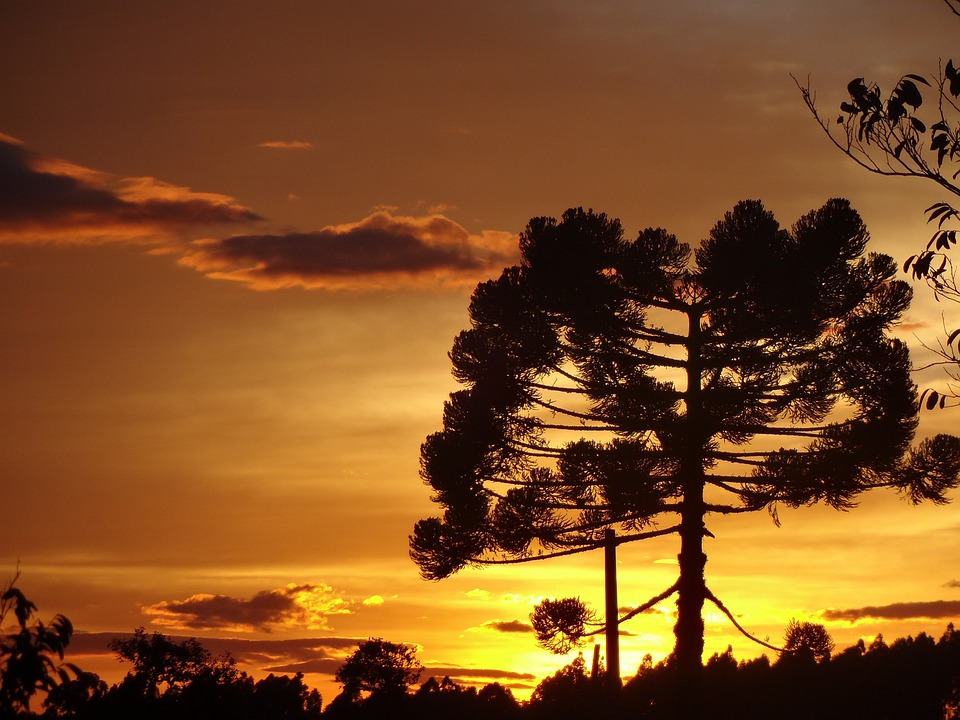
\includegraphics[width=.45\textwidth]{./imgs/img27.png}
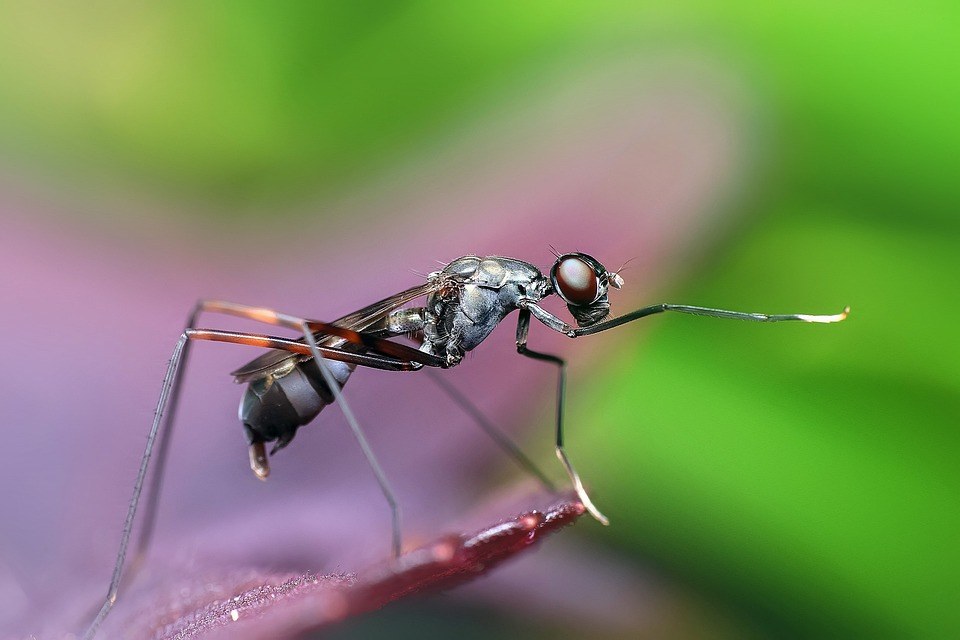
\includegraphics[width=.5\textwidth]{./imgs/img28.png}

\fonte{Árvore de araucária, que pode viver até 700 anos, e formiga, que vive até dois anos.}
}

\conteudo{Para entender quem somos, como funcionam nossa vida e nossa sociedade,
precisamos lembrar que só somos quem somos e fazemos o que fazemos por
causa do tempo. Também temos que saber que o tempo não é igual para
todos os seres. Para uma formiga, que vive no máximo dois anos, um ano é um
tempo muito grande e representa metade da sua vida. Para uma árvore de
araucária, que pode viver até 700 anos, um ano é muito pouco. O tempo da
humanidade também é diferente do tempo do homem. A humanidade existe há
mais de dois milhões de anos, enquanto o homem vive em média 70 anos.

São esses múltiplos tempos que vamos explorar neste módulo, além de sua
relação com o espaço que habitamos.}

%Disponível em: {\emph{https://pixabay.com/pt/photos/formiga-inseto-animal-artr\%c3\%b3pode-1130497/}} Acesso em: 23 fev. 2023

%Disponível em: {\emph{https://pixabay.com/pt/photos/arauc\%c3\%a1ria-pinheiro-manh\%c3\%a3-sol-633196/}} Acesso em: 23 fev. 2023

\colorsec{Atividades}


Observe as imagens para responder às questões de 1 a 3.

\begin{figure}[htpb!]
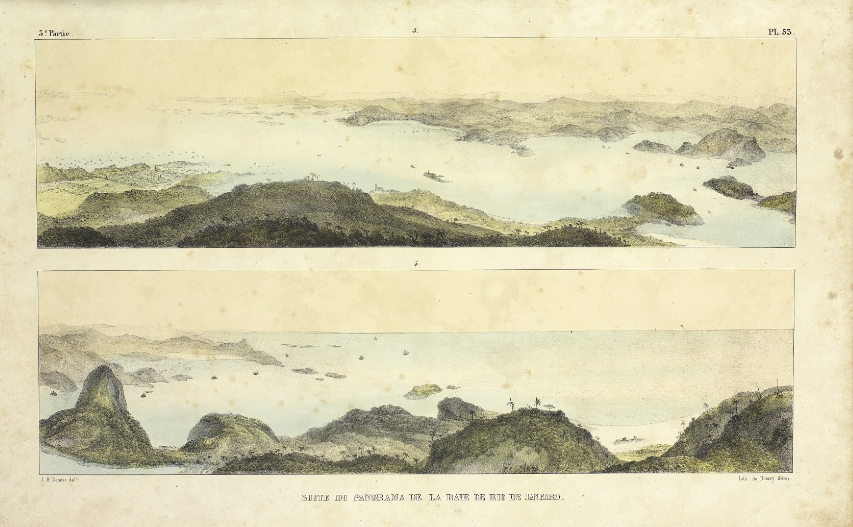
\includegraphics[width=.41\textwidth]{./imgs/img29.jpg}
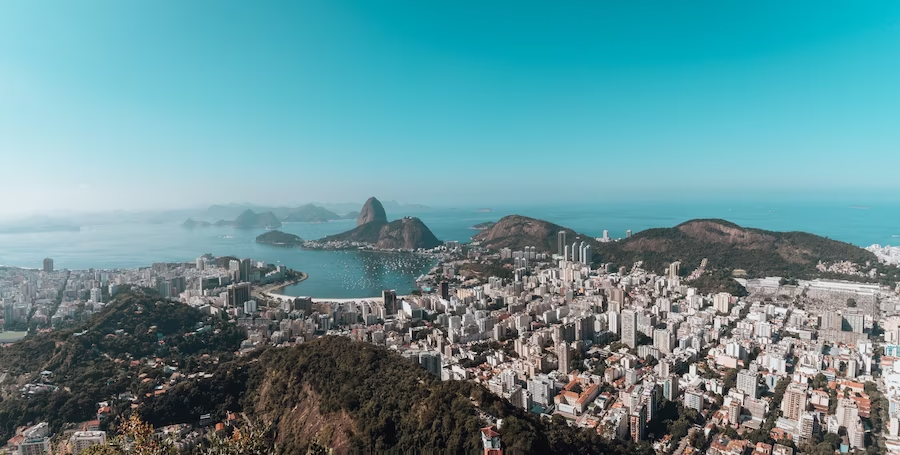
\includegraphics[width=.5\textwidth]{./imgs/img30.png}
\caption{Imagem 1: Thierry Frères. Sequência do panorama da Baía do Rio de Janeiro, 1839, Biblioteca Nacional. Gravura litografia, 12,4 x 44,6cm em f. 52,6 x 34,6. Imagem 2: Foto do Rio de Janeiro nos dias atuais.}
\end{figure}


\noindent{}As duas imagens representam o mesmo lugar, a Baía da cidade do Rio de
Janeiro, a primeira no ano de 1839, em uma gravura do artista Thierry
Frères, e a segunda em uma foto dos dias atuais.

\bigskip

\num{1} Quais mudanças você observa na imagem que ocorreram no espaço ao longo
do tempo? 

\reduline{Espera-se que os alunos apontem as mudanças na paisagem natural, tomada
pelos edifícios.\hfill}
\linhas{2}

\pagebreak
\num{2} Você sabe dizer o que aconteceu para que essas mudanças acontecessem?

\reduline{Espera-se que o aluno fale sobre a ocupação do homem no espaço natural,
podendo tocar em questões como habitação, migração, urbanização,
crescimento econômico, etc.
Aqui, incentive os alunos a entenderem a ação humana enquanto
transformadora do espaço ao longo do tempo.\hfill}

\num{3} Você já se deparou com alguma mudança no bairro ou na cidade onde vive?
A construção de novas casas, escolas, comércios, etc? Descreva e discuta
com seus colegas.

\reduline{Aqui os alunos devem trazer o debate para o seu cotidiano, falar sobre
as mudanças no espaço onde vive e perceber que ele está sempre em
construção e movimento ao longo do tempo.\hfill}
\linhas{1}

\noindent{}Observe a imagem, leia a reportagem, e, depois, discuta com seus colegas. Então, respondam às questões de 4 a 7.

\coment{Recomenda-se que esta atividade seja feita em duplas ou grupos de três alunos.}

\begin{figure}[htpb!]
\centering
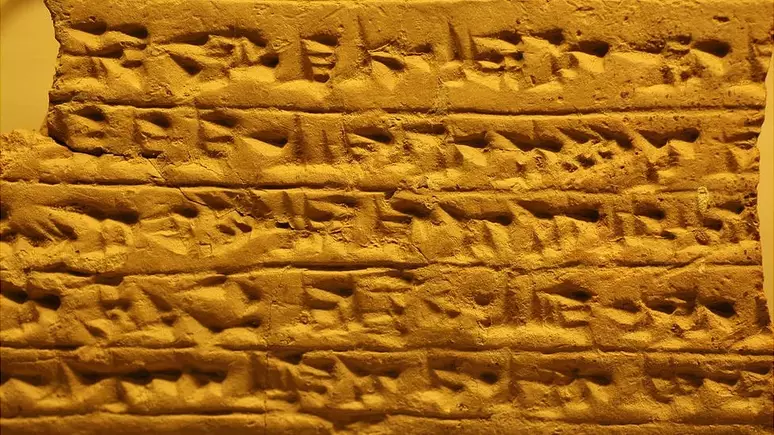
\includegraphics[width=.5\textwidth]{./imgs/img31.png}
%\caption{\emph{https://www.istockphoto.com/br/foto/antigo-cuneiforme-ass\%C3\%ADria-e-sum\%C3\%A9ria-da-mesopot\%C3\%A2mia-gm1128639883-297872773?phrase=escrita\%20cuneiforme}}
\end{figure}

\begin{quote}
\textbf{O que diz o primeiro documento escrito da história}

Na Antiguidade, acreditava-se que a escrita vinha dos deuses. Os gregos
pensavam tê-la recebido de Prometeus. Os egípcios, de Tot, o deus do
conhecimento. Para os sumérios, a deusa Inanna a havia roubado de Enki,
o deus da sabedoria. 

Mas, à medida que essa visão perdia crédito,
passou-se a investigar o que levou civilizações antigas a criar a escrita. Motivos religiosos ou artísticos? Ou teria sido para enviar mensagens a exércitos distantes?

{[}\ldots{}{]}

O enigma ficou mais complexo em 1929, após o arqueólogo alemão Julius Jordan desenterrar uma vasta biblioteca de tábuas de argila com figuras abstratas, um tipo de escrita conhecida como “cuneiforme”, com 5 mil anos de idade {[}\ldots{}{]}

\fonte{Terra. O que diz o primeiro documento escrito da história. Disponível em:
\emph{https://www.terra.com.br/byte/ciencia/o-que-diz-o-primeiro-documento-escrito-da-historia,91ff629390de632fb072b741c464fc55stmy8y08.html}.
Acesso em: 22 fev. 2023.}
\end{quote}

\pagebreak
\num{4} O que vocês entendem como um documento histórico?

\reduline{Espera-se que os alunos tenham a compreensão do documento histórico como
uma fonte onde estão registrados acontecimentos, costumes, pensamentos
dos seres humanos, entre outros.\hfill}

\num{5} Por que vocês acham que documentos como o reproduzido anteriormente são
importantes para nós hoje em dia?

\reduline{Aqui, os alunos devem ter o entendimento de que, a partir de documentos
como esse, podemos conhecer aspectos do passado da humanidade e entender
sua formação, seu desenvolvimento e seu crescimento até chegarmos ao tempo presente.\hfill}

\num{6} Vocês acham que a descoberta da escrita foi importante para os homens?
Por quê? O que ela nos permite fazer em nosso dia a dia?

\reduline{EsTa questão requer que os alunos entendam a revolução que o registro escrito representou
para o registro da memória humana. Podem aparecer respostas relacionadas ao
registro de contratos, ou outras questões mais burocráticas e legais, assim como questões mais amplas
como expressão individual, registro de leis, de mercadorias,
comunicação geral e ampla, envio de recados, confecção de provas etc.\hfill}

\num{7} Marquem com um X o que vocês acham que pode ser usado como um documento
histórico; depois, discutam com o professor e seus colegas o porquê
dessas escolhas.

\begin{boxlist}
\item
  Um livro de leis antigas.
\item
  Uma obra de arte em um museu.
\item
  Uma foto de família.
\item
  Um texto nas redes sociais.
\item
  Uma carta de amor.
\item
  Uma letra de música.
\item
  Um diário.
\end{boxlist}

\coment{O ideal é que os alunos marquem todas as alternativas. A ideia é que seja
discutido o fato de que qualquer registro da vida humana pode ser utilizado como
documento para entender a história dos homens. Assim, deve ser discutido
o poder da micro-história, ou seja, cada aluno deve entender que sua vida
pessoal, a de sua família, das pessoas de seu bairro, são reflexos de
aspectos históricos e também devem ser levadas em consideração.}

\pagebreak
Observe a imagem e leia o texto para responder às questões de 8 a 10.

\begin{figure}[htpb!]
\centering
%\begin{wrapfigure}{l}{.5\textwidth}
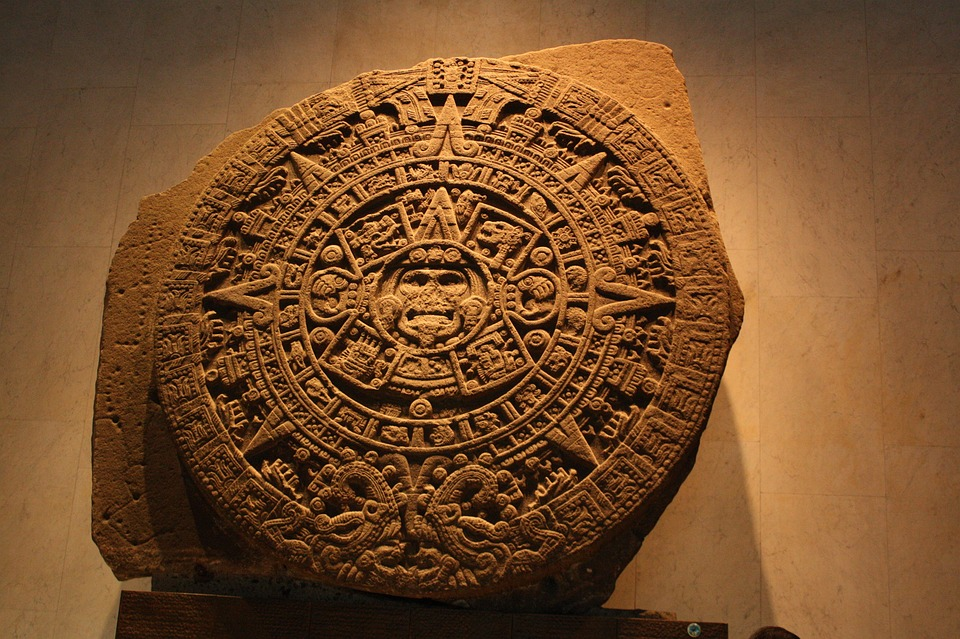
\includegraphics[width=.5\textwidth]{./imgs/img32.png}
%\caption{Disponível em: {\emph{https://pixabay.com/pt/photos/calend\%c3\%a1rio-asteca-asteca-escultura-642655/}} Acesso em: 23 fev. 2022}
%\end{wrapfigure}
\end{figure}

\noindent{}Você sabia que cada sociedade construiu seu próprio calendário? A imagem representa o calendário da sociedade Asteca, que viveu no território onde hoje é o México entre os anos de 1300 e 1500 d.C. Ele
é dividido em duas partes: uma baseada no ciclo do sol, que era utilizada para guiar os ciclos da agricultura, composta por 365 dias, e outra, de 260 dias, que guiava os rituais sagrados. O calendário que
utilizamos hoje em dia na sociedade ocidental vem da sociedade romana e foi criado em meados de 700 d.C. O calendário mais antigo do mundo é o chinês, baseado nos ciclos da lua e do sol (um ciclo completo tem a duração de 12 anos). O ano novo chinês, por exemplo, não é comemorado no dia 1 de janeiro, como estamos acostumados, mas sim entre os meses de janeiro e fevereiro, cada ano em um dia diferente. Texto original

Existem, por exemplo, calendários criados pelos povos indígenas brasileiros. Vamos descobrir como um desses calendários funciona.

O calendário indígena dos ciclos do rio Tiquié enfatiza fenômenos e ciclos que se relacionam com o cotidiano e a cultura desses povos indígenas. Para esses povos, o ano se divide em estações que são identificadas pela passagem de constelações astronômicas que se ligariam a fenômenos ecossistêmicos e climáticos. O ano, para eles, começa com a Enchente de Jararaca, no começo de novembro.

\fonte{Fonte de pesquisa: Infoamazônia. Calendário indígena dos ciclos do rio Tiquié. Disponível em:
\emph{https://infoamazonia.org/project/calendario-indigena-dos-ciclos-do-rio-tiquie/}.
Acesso em: 22 fev. 2023.}

\num{8} O que é um calendário? Qual é sua função em cada sociedade?

\reduline{Aqui, o aluno deve falar sobre o calendário e sua relação com a marcação
do tempo e com a organização da sociedade.\hfill}
\linhas{3}

\num{9} Qual é a principal importância do calendário para o povo indígena brasileiro descrito no texto?

\reduline{Aqui, espera-se que o aluno fale sobre a relação dos povos indígenas
brasileiros com o clima e com as estações do ano.\hfill}

\num{10} Aponte duas características de cada calendário mencionado nos textos:

Calendário Asteca:

\begin{enumerate}
\item \rosa{agricultura baseada no ciclo do sol}

\item \rosa{função religiosa e sagrada}
\end{enumerate}

Calendário Romano:

\begin{enumerate}
\item \rosa{Aqui o aluno pode colocar qualquer característica do calendário
ocidental atual: 12 meses,}

\item \rosa{4 estações, 365 dias, etc. As informações não
estão no texto, então o professor deve lembrar que este é o calendário
que eles utilizam no dia a dia.}
\end{enumerate}

Calendário Chinês:

\begin{enumerate}
\item \rosa{Baseado no ciclo da lua e do sol}

\item \rosa{Duração de 12 anos}
\end{enumerate}

Calendário indígena brasileiro:

\begin{enumerate}
\item \rosa{Dividido por estações}

\item \rosa{baseado em aspectos da natureza, peixes, chuvas etc)}
\end{enumerate}

\colorsec{Treino}

\num{1} A micro-história é como uma análise em miniatura da história. Ela se caracteriza pelo estudo de partes da história sem o envolvimento de personalidades ou de eventos de escala mundial. Um
exemplo é o estudo da vida de pessoas comuns, como camponeses da Idade Média e trabalhadores que, em vida, não tiveram notoriedade.

Um objeto da micro-história, além dos camponeses da Idade Média como
aponta o texto, pode ser:

\begin{escolha}
\item o conjunto de decisões de presidentes importantes.

\item uma guerra entre grandes sociedades.

\item o cotidiano de empregadas domésticas.

\item a ocupação de continentes desconhecidos.
\end{escolha}

\coment{BNCC: EF05HI07 - Identificar os processos de produção,
hierarquização e difusão dos marcos de memória e discutir a presença
e/ou a ausência de diferentes grupos que compõem a sociedade na nomeação
desses marcos de memória.}

\num{2} Leia o texto.

\begin{quote}
\textbf{Dicionário histórico dos nomes das ruas de Guarulhos - São Paulo}\\
Tipo: Rua\\
Denominação atual: Rua Inhuma\\
Denominação antiga: Rua Cinco\\
Bairro: Vila Dinamarca, Água Chata\\
Ato legal: Decreto nº 5.168, de 31 de dezembro de 1975\\
Verbete: Sua denominação pode ser entendida a partir de duas
referências. A primeira faz alusão à cidade de Inhuma, no estado do
Piauí, e a segunda à ave anhuma, também conhecida como inhuma, presente
na bandeira de Guarulhos. Inhuma é um termo de origem tupi e significa
ave ou pássaro preto. O município piauiense localiza-se a
aproximadamente 259 km da capital, Teresina. A possibilidade de a rua
ter recebido esse nome em homenagem ao município piauiense é grande;
Guarulhos e outras regiões a leste da cidade de São Paulo receberam
grande migração nordestina. Quanto à ave, é símbolo do estado de Goiás.
É nativa da América do Sul, vivendo em áreas à beira de rios, lagos e
mangues.

\fonte{Dicionário histórico das ruas de Guarulhos. Rua Inhuma. Disponível em:
\emph{https://dicionarioruasguarulhos.wordpress.com/rua-inhuma/}.
Acesso em: 23 fev. 2023.}
\end{quote}

Como aponta o texto, o nome da Rua Inhuma, na cidade de Guarulhos, pode
ter sido dado por dois motivos:

\begin{escolha}
\item hábitos alimentares e vestimentas tradicionais.

\item importância do comércio e cultura popular.

\item origem dos moradores e símbolo da cidade.

\item localização na cidade e formato das casas.
\end{escolha}

\coment{BNCC: EF05HI01 - Identificar os processos de formação das culturas e dos povos, relacionando-os com o espaço geográfico ocupado.}

\num{3}

\begin{quote}
Chove muito, o verão não acontece. A roça também não queima, porque a
chuva é muita. Nossos avôs já diziam isso. Parece que a nossa época não
é boa, por isso a chuva não para de cair.

Antes não era assim. Antigamente, quando meu pai ainda era vivo, não era
como agora. Só agora é desse jeito... Por que o tempo de hoje se
transformou?

Talvez nosso dono altere o tempo de hoje, o tempo vai mudar, por isso
chove muito. Nosso dono vai trocar a terra. A terra será renovada, disse
o nosso dono, por isso a terra queimará. A terra queimará... {[}\ldots{}{]}

\fonte{Seremete Wajãpi. Povos Indígenas no Brasil. Disponível em:
\emph{https://pib.socioambiental.org/pt/\%22O\_tempo\_vai\_mudar,\_por\_isso\_chove\_muito.\_Nosso\_dono\_vai\_trocar\_a\_terra\%22}
Acesso em: 23 fev. 2023}
\end{quote}

A declaração do indígena Seremete Wajãpi mostra que, para sua comunidade, o tempo está diretamente ligado a

\begin{minipage}{.5\textwidth}
\begin{escolha}
\item acontecimentos da natureza.

\item guerras entre povos.

\item rituais de cura.

\item relações das famílias.
\end{escolha}
\end{minipage}
\sidetext{BNCC: EF05HI08 - Identificar formas de marcação da passagem do
tempo em distintas sociedades, incluindo os povos indígenas originários
e os povos africanos.}

\chapter{Natureza e meio ambiente}
\markboth{Módulo 2}{}

\coment{Habilidades da BNCC: EF05GE03, EF05GE10, EF05GE11, EF05GE12.}

\colorsec{Eixo de conhecimento do SAEB}

\begin{itemize}
\item Natureza e questões socioambientais.
\end{itemize}

\conteudo{O homem está separado da natureza? O lugar em que vivemos faz parte de
florestas, campos, rios e mares onde vivem os animais? Mesmo que não
vivamos em nosso dia a dia em contato direto com a natureza, nossas
ações impactam na preservação ou na destruição dela ao nosso redor. Tudo o
que usamos em nosso cotidiano vem da natureza. Esta folha de papel, por
exemplo, em que você está lendo este texto, veio de uma árvore, assim
como o lápis que está no seu estojo. Isso quer dizer que estamos
destruindo a natureza escrevendo em nossos cadernos? Não, mas quer dizer
que precisamos trabalhar pelo equilíbrio do uso de nossos recursos
naturais. Devemos sempre pensar em como podemos passar por esse processo
de maneira \textbf{sustentável}.

Mas como ser sustentável? O que isso significa?

\begin{wrapfigure}{l}{.5\textwidth}
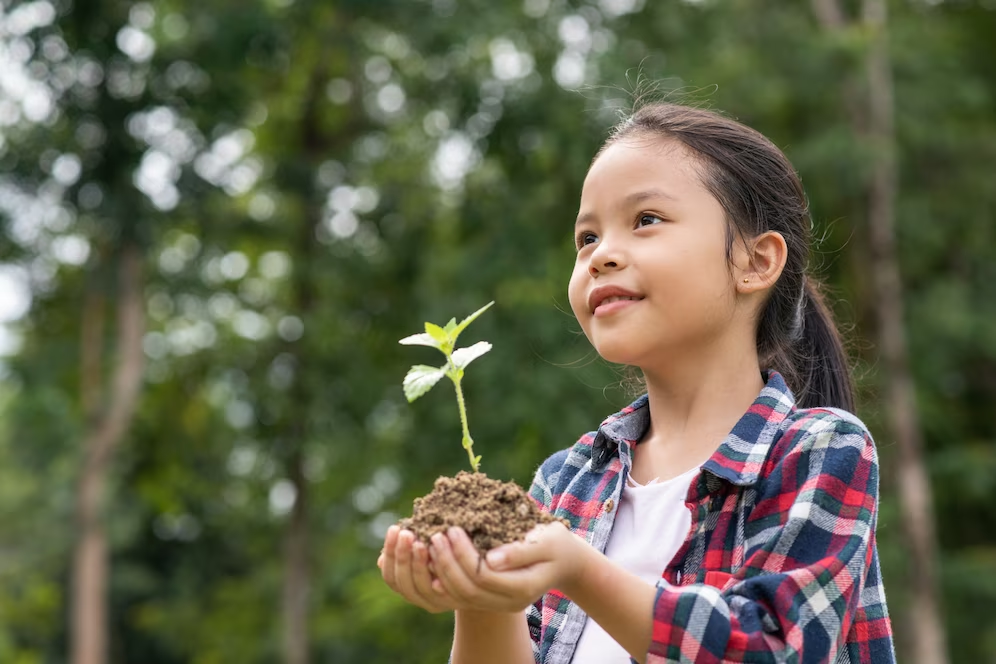
\includegraphics[width=.48\textwidth]{./imgs/img33.png}
%\caption{\emph{https://br.freepik.com/fotos-gratis/menina-asiatica-segurando-planta-e-solo\_5598508.htm\#query=preserva\%C3\%A7\%C3\%A3o\&position=9\&from\_view=search\&track=sph}}
\end{wrapfigure}

Para cooperarmos com a sustentabilidade precisamos garantir que, mesmo utilizando os
recursos naturais para nossa vida no presente, devemos cuidar para que eles não acabem. Isso
porque as pessoas vão precisar deles no futuro! Imagine se cinquenta anos
atrás nossos avós tivessem acabado com todas as árvores do planeta e
tivessem usado toda água potável do mundo... como viveríamos hoje?

Neste módulo vamos trabalhar com atividades que relacionam a vida humana
com a natureza. Afinal, somos todos parte do mesmo planeta e precisamos
uns dos outros para sobreviver.}

\colorsec{Atividades}

Vamos ler uma reportagem de 2020 para responder às atividades de 1 a 3.

\begin{quote}
\textbf{Expansão urbana provoca encontros incomuns com onças-pardas}

Imagine a emoção de ficar frente a frente com uma onça. Com certeza a
adrenalina predomina no instante do encontro. No entanto, quando o
flagrante é feito em áreas urbanas, um sinal vermelho se acende, afinal,
esse não é o habitat ideal para um felino selvagem. Infelizmente estes
casos são cada vez mais frequentes devido à expansão urbana desenfreada,
construções de rodovias que dividem áreas verdes e desmatamento
constante. {[}\ldots{}{]}

“É importante que ele seja reintroduzido logo, para buscar o habitat
natural. Devemos trabalhar essa consciência ambiental e atuar de forma
correta para que a gente não prejudique nem a natureza e nem o animal,
que não tem culpa de nada do que está acontecendo”. {[}\ldots{}{]}

\fonte{G1. Expansão urbana provoca encontros incomuns com onças-pardas. Disponível em: \emph{https://g1.globo.com/sp/campinas-regiao/terra-da-gente/noticia/2020/01/29/expansao-urbana-provoca-encontros-incomuns-com-oncas-pardas.ghtml}. Acesso em: 22 mar. 2023.}
\end{quote}

\num{1} Agora, vamos investigar melhor esse fenômeno. Qual você acha que foi a principal ação humana responsável por esse acontecimento?

\reduline{Espera-se que o aluno fale sobre a expansão urbana na natureza, sobre o
crescimento das cidades e a ocupação de territórios em que,
originalmente, habitavam animais selvagens.\hfill}
\linhas{1}

\num{2} Como você acha que o crescimento de áreas urbanas afeta a natureza e os
animais que vivem ao redor?

\reduline{Aqui, proponha uma reflexão tanto sobre a fauna quanto sobre a flora. Faça os
alunos refletirem sobre questões mais amplas como desmatamento,
poluição, invasão territorial etc.\hfill}
\linhas{1}

\num{3} Você acha que a expansão urbana pode trazer perigo aos próprios seres
humanos? Se sim, por quê?

\reduline{Volte ao conteúdo da reportagem do caso da onça parda. Fale sobre
os perigos do contato entre homens e animais selvagens. O objetivo é que
o aluno entenda que as ameaças da expansão urbana desenfreada não estão
restritas aos animais.\hfill}
\linhas{2}

\colorsec{Atividade 2}

\coment{BNCC: EF05GE11.}

\noindent{}Agora, observe a imagem, e, seguida, leia a reportagem de 2022. Então, responda às atividades de 4 a 8.

\begin{figure}[htpb!]
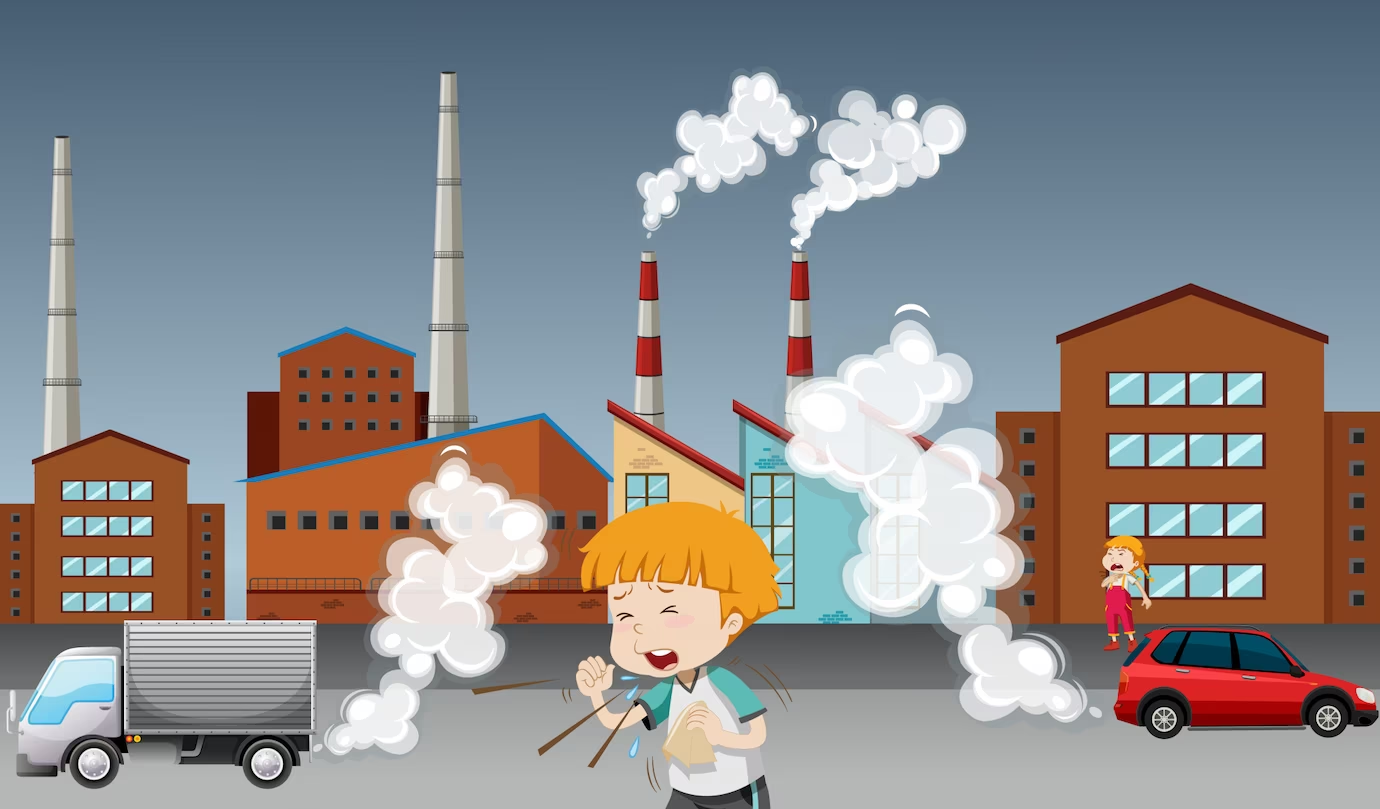
\includegraphics[width=\textwidth]{./imgs/img34.png}
%\caption{\emph{https://br.freepik.com/vetores-gratis/cartaz-de-aquecimento-global-com-crianca-e-fabrica\_5837841.htm\#query=polui\%C3\%A7\%C3\%A3o\%20escola\&position=8\&from\_view=search\&track=ais}}
\end{figure}

\begin{quote}
\textbf{Poluição em escolas em Diadema, na Grande SP, é quase três vezes maior
do que o recomendado, aponta pesquisa.}

Um estudo realizado em cinco escolas públicas de Diadema, na Grande São
Paulo, mostra que os níveis de poluentes no ar da cidade estão muito
acima do normal. O nível de poluição está em 40 microgramas diários de
poluentes e, segundo a Organização Mundial da Saúde (OMS), o
recomendável seria ter até 15 microgramas. {[}\ldots{}{]} Para medir o nível de
poluição, as escolas receberam um equipamento para monitorar os
poluentes. {[}\ldots{}{]}

“Foi uma surpresa porque a nossa escola é bastante arborizada e, quando
vimos os resultados, foi surpreendente. Imaginávamos que fosse melhor.”,
afirma Carolina de Paula Lusa, diretora da escola municipal de educação
básica Carolina Maria de Jesus. {[}\ldots{}{]}

\fonte{Bruna Vieira. G1. Poluição em escolas em Diadema, na Grande SP, é quase três vezes maior do que o recomendado, aponta pesquisa. Disponível em: \emph{https://g1.globo.com/sp/sao-paulo/noticia/2022/07/06/poluicao-em-escolas-em-diadema-na-grande-sp-e-quase-tres-vezes-maior-do-que-o-recomendado-aponta-pesquisa.ghtml}.
Acesso em: 23 fev. 2023}
\end{quote}

\num{4} Descreva o que você observa na imagem.

\reduline{Espera-se que o aluno descreva o ambiente urbano e seus componentes, os
carros e as indústrias, além das personagens humanas e suas expressões.\hfill}

\num{5} Na sua opinião, como podemos relacionar os elementos da imagem ao
acontecimento relatado na reportagem?

\reduline{Aqui, o aluno deve relacionar a poluição observada na imagem em
decorrência dos automóveis e indústrias com a qualidade do ar observada
na escola.\hfill}
\linhas{1}

\num{6} Como podemos explicar, no caso de Diadema, que mesmo a escola tendo
bastante árvores, os níveis de poluentes estão acima do normal?

\reduline{Espera-se que o aluno situe a escola dentro do ambiente da cidade, ou
seja, que ele entenda que as interferências humanas no ambiente externo
à escola afetam o perímetro escolar. Mesmo a escola sendo urbanizada,
pode haver indústrias, automóveis e outros fatores ao redor da escola
que comprometam a salubridade naquele local.\hfill}
\linhas{1}

\num{7} Qual o perigo que a poluição do ar traz para as crianças nas escolas?

\reduline{Como na imagem acima, as crianças podem ficar doentes e ter a qualidade
da respiração afetada pelo ar poluído, tornando insalubre o ambiente escolar
frequentado todos os dias por elas.\hfill}

\num{8} Marque com um X as medidas do governo e da população que podem ajudar na
diminuição da poluição do ar nas cidades.

\begin{boxlist}
\boxitem{X}
  Incentivar o uso de transportes coletivos.
\boxitem{X}
  Diminuir as queimadas em plantações.
\boxitem{\white{X}}
  Asfaltar as ruas da cidade.
\boxitem{X}
  Plantar árvores em áreas desmatadas.
\boxitem{\white{X}}
  Melhorar o sistema de esgoto.
\end{boxlist}

\coment{Nesta etapa da atividade, é interessante que sejam debatidos com os
alunos cada ponto colocado, entendendo no que exatamente eles auxiliam a
sociedade. Os transportes, pela diminuição de emissão de poluentes em
carros privados; as queimadas, pela diminuição da emissão de gases
tóxicos que resultam da ação; as árvores, pois melhoram a
qualidade do ar a partir do processo de fotossíntese.

Recomenda-se que esta atividade seja feita em grupos. Isso para que os
alunos compartilhem suas experiências e, juntos, busquem soluções.}

\pagebreak
Observe as imagens e responda às questões de 9 a 13 com seus colegas.

\begin{figure}[htpb!]
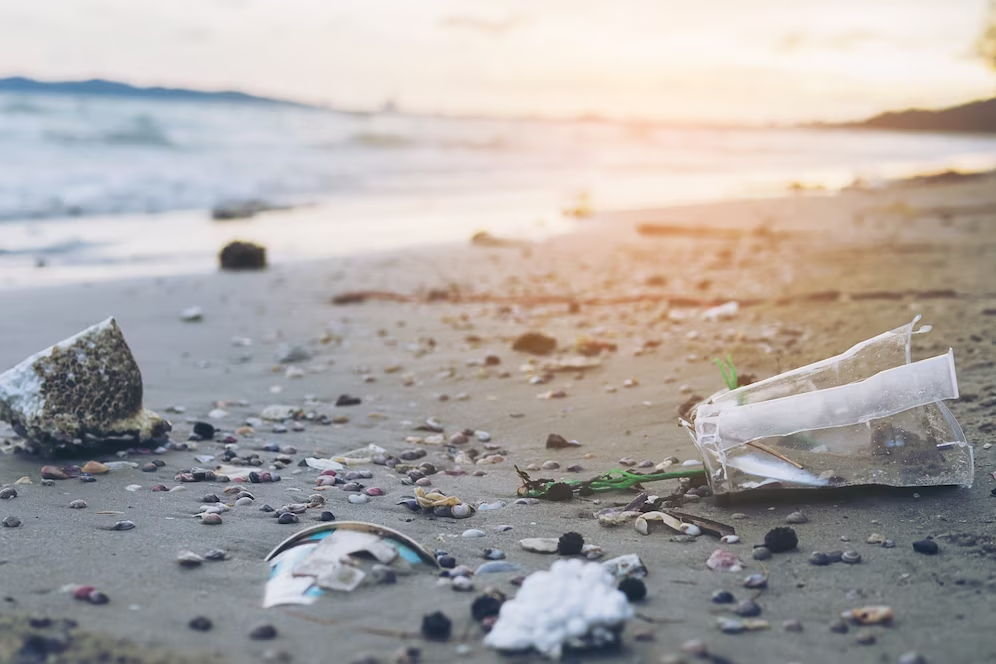
\includegraphics[width=.5\textwidth]{./imgs/img35.png}
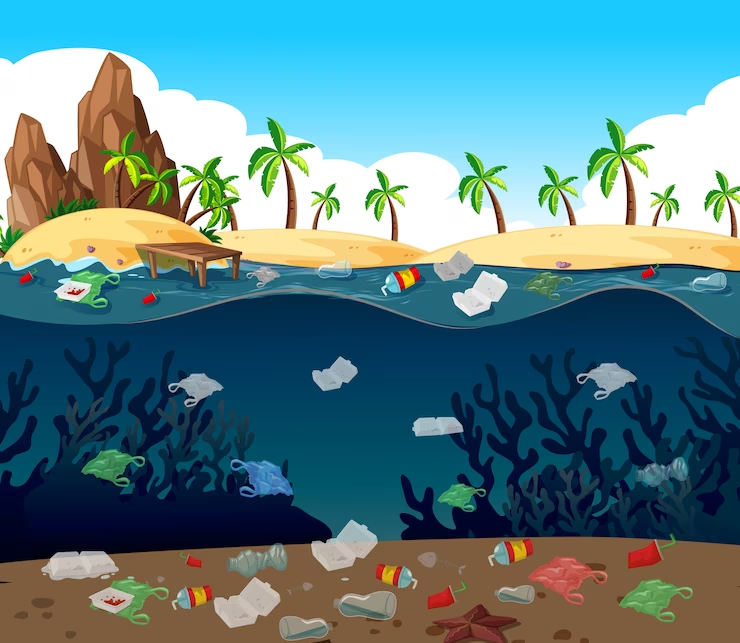
\includegraphics[width=.38\textwidth]{./imgs/img36.png}
\caption{Imagem 1 e Imagem 2}
\end{figure}

%\emph{https://br.freepik.com/fotos-gratis/lixo-na-areia-da-praia-mostrando-o-problema-de-poluicao-ambiental\_3805894.htm\#query=praia\%20polu\%C3\%ADda\&position=3\&from\_view=search\&track=ais}

%\emph{https://br.freepik.com/vetores-gratis/poluicao-da-agua-com-sacos-de-plastico-no-oceano\_7026496.htm\#query=mar\%20polu\%C3\%ADdo\&position=7\&from\_view=search\&track=ais}

\num{9} Você já foi ou conhece alguém que foi à praia? Se sim, como você ou essa
pessoa descreveriam essa experiência e a paisagem? Se não, como você
imagina que seria?

\reduline{Essa questão pretende iniciar o debate entre os alunos. Lembrando de
suas experiências, eles poderão se relacionar de maneira pessoal com as
questões em seguida.\hfill}
\linhas{2}

\num{10} Agora, descrevam o que vocês veem nas imagens apresentadas anteriormente.

\reduline{Espera-se que os alunos apontem a grande quantidade de resíduos
descartados nas paisagens.\hfill}
\linhas{2}

\num{11} Como vocês acham que a imagem 1 se relaciona com a imagem 2?

\reduline{Aqui, espera-se que o aluno relacione a causa à consequência: ao jogar
lixo na praia, estão colaborando para o acúmulo de lixo no fundo do mar.\hfill}
\linhas{1}

\num{12} Quais os impactos que a ação de jogar lixo na praia tem sobre a natureza e os animais que vivem nela? Cite três.

\begin{enumerate}
\item \linhas{2}

\item \linhas{2}

\item \linhas{2}
\end{enumerate}

\coment{Estimule os alunos a pensar nas consequências dessa ação tanto para o
homem quanto para os animais e a vegetação local. Podem ser citados:
turismo, morte de animais e risco de extinção de espécies, poluição da
água do mar e dos peixes a serem consumidos pelos humanos etc.}

\num{13} Converse com os colegas e aponte duas ações que podem ser feitas para
diminuir o lixo nas praias e nos mares.

\reduline{Aqui podem entrar tanto ações individuais, como descartar o lixo em
local adequado quando visitar a praia, quanto governamentais, como
promover ações de retirada do lixo das praias, estimular a reciclagem,
etc.\hfill}

\colorsec{Treino}

\num{1}

\begin{quote}
\textbf{Ubatuba começa a cobrar taxa ambiental de R\$ 13 por veículo
nesta quarta-feira}\\
A cobrança da taxa será feita por um sistema semelhante ao da cobrança
eletrônica (Sem Parar) dos pedágios de rodovias, instalados nos
principais acessos da cidade.

A partir da zero hora desta quarta-feira, 8, turistas e visitantes terão
de pagar taxa para permanecer por mais de 4 horas em Ubatuba, no litoral
norte de São Paulo. A cidade, um dos principais destinos do verão
paulista, tem 102 praias catalogadas. A prefeitura criou uma taxa de
preservação ambiental para compensar os impactos gerados pelo alto fluxo
de turistas, sobretudo na alta temporada, como agora. A tarifa básica
para carros é de R\$ 13 por período (entrada e saída). {[}\ldots{}{]}

\fonte{EXAME. Ubatuba começa a cobrar taxa ambiental de R\$ 13 por veículo nesta quarta-feira. Disponível em: \emph{https://exame.com/}.
Acesso em: 6 fev. 2023}
\end{quote}

Segundo o texto, a cobrança da taxa ambiental pela prefeitura tem como
objetivo

\begin{escolha}
\item aumentar o número de turistas na região.

\item controlar a criminalidade na cidade.

\item diminuir o consumo de peixes e frutos do mar.

\item garantir a preservação das praias locais.
\end{escolha}

\coment{BNCC: EF05GE10 - Reconhecer e comparar atributos da qualidade ambiental e algumas formas de poluição dos cursos de água e dos oceanos (esgotos,
efluentes industriais, marés negras etc.).}

\num{2} Observe a imagem.

\begin{figure}[htpb!]
\centering
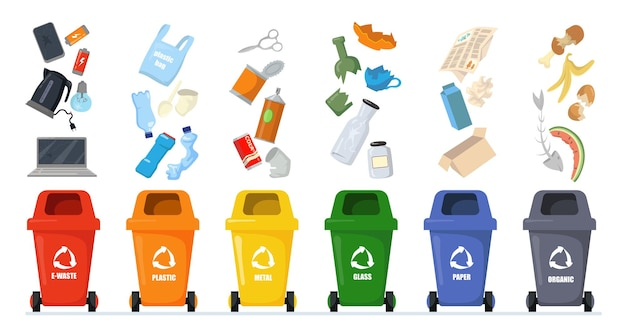
\includegraphics[width=.5\textwidth]{./imgs/img37.jpg}
%\caption{\emph{https://br.freepik.com/vetores-gratis/conjunto-de-triagem-de-lixo\_13146308.htm\#query=reciclagem\&position=4\&from\_view=search\&track=sph}}
\end{figure}

A imagem ilustra um elemento que impacta o seguinte processo:

\begin{minipage}{.5\textwidth}
\begin{escolha}
\item saneamento básico.

\item industrialização.

\item reciclagem.

\item urbanização.
\end{escolha}
\end{minipage}
\sidetext{BNCC: EF05GE11 - Identificar e descrever problemas ambientais que ocorrem no
entorno da escola e da residência (lixões, indústrias poluentes,
destruição do patrimônio histórico etc.), propondo soluções (inclusive
tecnológicas) para esses problemas.}

\num{3}

\begin{quote}
\textbf{Estatuto da Cidade, Lei No 10.257, de 10 de julho de 2001}

Art. 2º A política urbana tem por objetivo
ordenar o pleno desenvolvimento das funções sociais da cidade e da
propriedade urbana, mediante as seguintes diretrizes gerais:

XVII - estímulo à utilização, nos parcelamentos do solo e nas
edificações urbanas, de sistemas operacionais, padrões construtivos e
aportes tecnológicos que objetivem a redução de impactos ambientais e a
economia de recursos naturais.

\fonte{Jusbrasil. Artigo 2 da Lei nº 10.257 de 10 de julho de 2001. Disponível em: \emph{https://exame.com/}.
Acesso em: 6 fev. 2023.}
\end{quote}

O trecho do Estatuto da Cidade reproduzido anteriormente tem como objetivo
equilibrar o desenvolvimento urbano com o (a)

\begin{minipage}{.5\textwidth}
\begin{escolha}
\item ampliação das escolas.

\item crescimento da população.

\item preservação da natureza.

\item produção de alimentos.
\end{escolha}
\end{minipage}
\sidetext{BNCC: EF05GE03 - Identificar as formas e funções das cidades e
analisar as mudanças sociais, econômicas e ambientais provocadas pelo
seu crescimento.}

\chapter{Tudo é diverso}
\markboth{Módulo 3}{}

\coment{Habilidades da BNCC: EF05GE02, EF05HI03, EF05HI10.}

\colorsec{Eixo de conhecimento do SAEB}

\begin{itemize}
\item Culturas, identidades e diversidades.
\end{itemize}


\conteudo{Todas as pessoas do planeta vivem de maneira igual? Você acorda, vive o
dia, se alimenta e dorme todos os dias. Isso parece ser igual para
você, para mim, e para uma pessoa do outro lado do planeta. Isso quer
dizer que somos iguais? Apesar de sermos todos seres humanos, o modo
como levamos nossas vidas depende de vários fatores. Por exemplo: uma
criança que nasce em uma comunidade na beira do rio está muito mais
acostumada a comer peixe no seu dia a dia do que uma criança nascida em
uma fazenda no interior, que come ovos de galinha e carne de boi. Uma
criança que vive em uma cidade muito fria se veste com roupas muito
mais pesadas do que uma criança que vive em uma cidade muito quente. O
que comemos, o modo como nos vestimos, como aproveitamos a vida, tudo depende
do lugar onde crescemos.

\begin{wrapfigure}{l}{.5\textwidth}
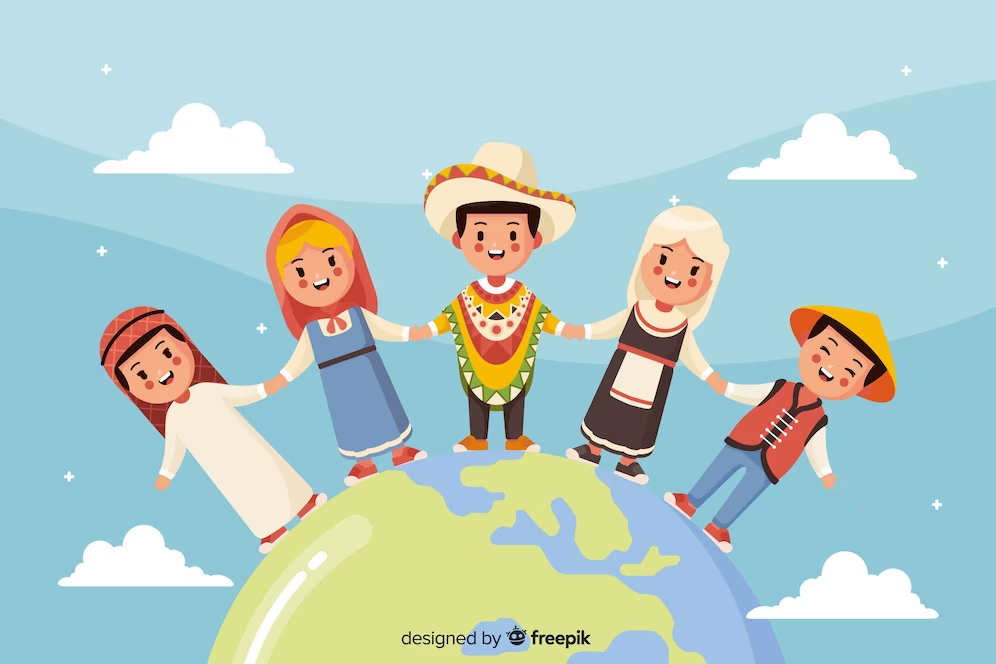
\includegraphics[width=.48\textwidth]{./imgs/img38.png}
%\caption{\emph{https://br.freepik.com/vetores-gratis/fundo-plano-de-dia-de-paz-com-as-criancas\_5189550.htm\#query=crian\%C3\%A7a\%20cultura\&position=4\&from\_view=search\&track=ais}}
\end{wrapfigure}

Neste módulo vamos trabalhar para entender nossas diferenças e
semelhanças, pensar em de onde vem nossa cultura e em como podemos viver em
comunidade e respeitar o próximo.


\vspace{2cm}}

\pagebreak
\colorsec{Atividades}

Observe as imagens, leia a reportagem sobre o Carnaval e, em seguida,
discuta com os colegas. Depois, responda às questões de 1 a 5.

\begin{figure}[htpb!]
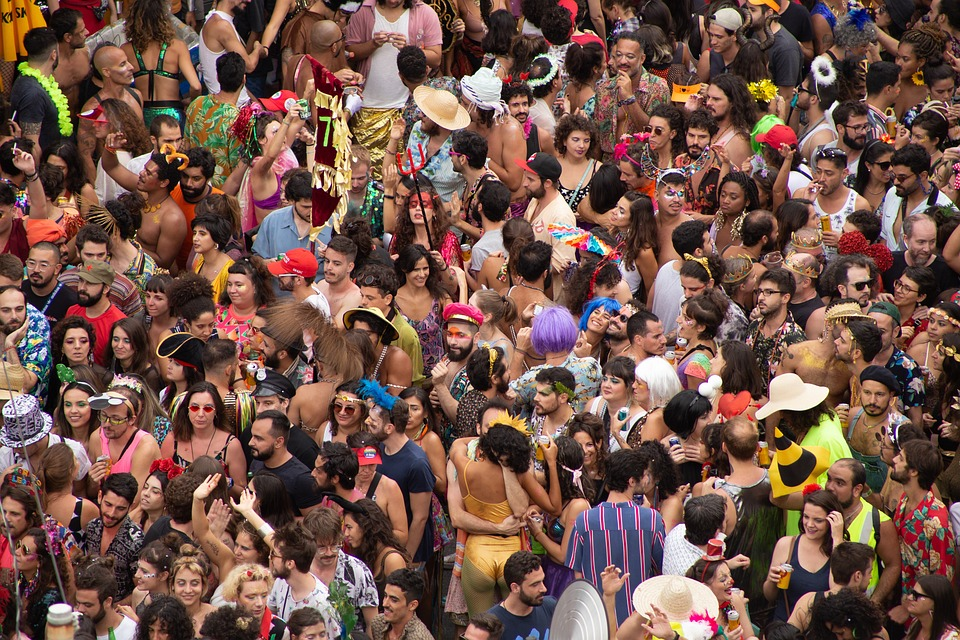
\includegraphics[width=.5\textwidth]{./imgs/img39.png}
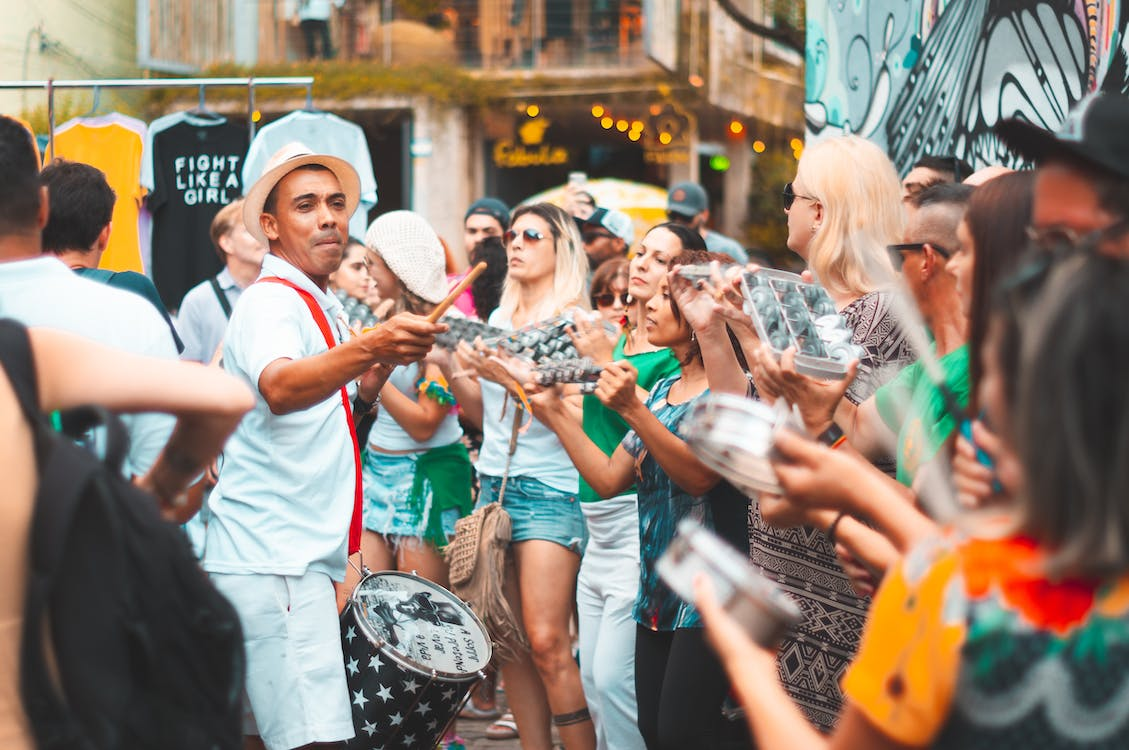
\includegraphics[width=.5\textwidth]{./imgs/img40.png}
%\caption{\emph{https://pixabay.com/pt/photos/pessoas-multid\%c3\%a3o-celebra\%c3\%a7\%c3\%a3o-6622786/}}
%\caption{\emph{https://www.pexels.com/pt-br/foto/homem-vestindo-camisa-polo-branca-e-chapeu-1974100/} }
\end{figure}

\begin{quote}
{[}...{]} em 1846, já existia uma prática que foi absorvida ao Carnaval: o Zé
Pereira, que era uma pessoa que saía andando pelas ruas batendo bumbo e
tambores. {[}\ldots{}{]} O “Zé
Pereira” era considerado um “Carnaval do Pobre”, já que não era
preciso convite {[}\ldots{}{]}, bastava uma pessoa e um tambor
para a festa começar nas ruas.

No início do século 20, a festa de rua mudou nas capitais brasileiras.
Isso porque a própria rua mudou. No Rio de Janeiro, por exemplo, a
Avenida Central foi aberta entre 1903 e 1906. O espaço passou das ruas
estreitas para as largas avenidas. Apenas para abrir a Avenida Central,
foram demolidas entre 600 e 3 mil casas, desabrigando mais de 20 mil
pessoas mais pobres, levando-as para regiões mais afastadas. {[}\ldots{}{]}

Embora tenha sido idealizada para {[}\ldots{}{]} os ricos {[}\ldots{}{]}, a reurbanização trouxe também os mais pobres para aproveitar
as ruas e calçadas nos dias de folga. O Carnaval e o urbanismo se
encontraram. A Avenida Central, feita com calçadas largas, tinha os
pedestres e o comércio em foco. E, durante o Carnaval, tornou-se o eixo
dos blocos e cordões. Em Salvador, o mesmo aconteceu na Avenida Sete de
Setembro e em volta do Farol da Barra. {[}\ldots{}{]}

\fonte{Da Redação. Habitability. Carnaval e urbanismo: uma história que se mistura no Brasil. Disponível em:
\emph{https://habitability.com.br/carnaval-e-urbanismo-uma-historia-que-se-mistura-no-brasil/}.
Acesso em: 23 fev. 2023.}
\end{quote}

\num{1} Você sabe o que é carnaval? Já participou de algum? Escreva e
compartilhe sua experiência com seus colegas.

\reduline{Espera-se que os alunos tragam experiências pessoais, falem do que
entendem por carnaval. Cabe ao docente guiar a discussão.\hfill}
\linhas{3}

\pagebreak

\num{2} O que a figura de “Zé Pereira” simboliza dentro das comemorações de
carnaval?

\reduline{Aqui, o professor deve guiar a reflexão dos alunos, pois a associação é um pouco mais complexa. Deve-se falar sobre a relevância
e a importância do povo para essa comemoração. Zé pereira simboliza o
cidadão comum, que manifesta a cultura do carnaval de rua. Pode-se falar também sobre a importância da ocupação do espaço da rua por
esse personagem.\hfill}
\linhas{2}

\num{3} Qual é a ação do governo descrita pelo texto na cidade que muda o
funcionamento do carnaval no Rio de Janeiro ao longo do tempo?

\reduline{Aqui o aluno deve falar sobre a abertura das ruas e a criação de largas
avenidas.\hfill}
\linhas{2}

\num{4} Cite uma consequência negativa e uma positiva dessa mudança.

\reduline{Negativa: Desabrigou pessoas.\\
Positiva: Maior espaço de reunião da população nas festividades.
Ocupação em massa do espaço público.\hfill}

\num{5} Você já viu outros tipos de eventos em seu bairro ou em sua cidade que
ocuparam e fecharam as ruas? Cite e discuta com os colegas.

\reduline{Aqui, espera-se que os alunos busquem na memória situações em que viram
as ruas ocupadas pela população, como feiras de rua, festas de São João,
festas de ano novo, manifestações populares, eventos esportivos etc.\hfill}
\linhas{2}

\bigskip
\noindent{}Leia os textos a seguir sobre o Projeto Integrado Entrada da Cidade
(Piec), projeto da prefeitura da cidade de Porto Alegre, no Rio Grande
do Sul. Depois, responda às questões de 6 a 9.

\pagebreak
\begin{quote}
\textbf{Texto 1}\\
\textbf{Entrada da Cidade, cara nova na chegada à Capital}

{[}\ldots{}{]} O Projeto Integrado Entrada da Cidade (Piec) visa ao desenvolvimento
urbano, socioeconômico e ambiental da Região Humaitá-Navegantes, com um
investimento de R\$ 140 milhões. As ações voltadas à habitação atendem
3.775 famílias com um investimento de R\$ 71,4 milhões; 3.061 são novas
casas e 714 lotes urbanizados.

\fonte{Prefeitura de Porto Alegre. Entrada da cidade, cara nova na chegada à capital. Disponível em:
\emph{http://www2.portoalegre.rs.gov.br/demhab/default.php?p\_secao=101}.
Acesso em: 23 fev. 2023.}
\end{quote}

\begin{quote}
\textbf{Texto 2}\\
A referência ao “morro” e ao “asfalto” é talvez uma das imagens mais
utilizadas para indicar a divisão entre pobres e ricos nas cidades
brasileiras. Se essas imagens funcionam como representações das
delimitações espaciais entre pobres e ricos, elas também generalizam o
que há no asfalto e no morro. A implementação do PIEC junto aos
moradores e especificamente com relação à questão das moradias consistiu
na mudança das famílias que viviam em áreas consideradas “de risco”
para os novos condomínios residenciais. Ao andar pelas ruas da Entrada
da Cidade (EC) atentando ao pertencimento racial das famílias que moram
ali é possível identificar uma certa geografia racial vivida no
cotidiano, ou, se preferirmos, é possível identificar o papel da
identidade racial na configuração da geografia daquele espaço. A
espacialização que divide algumas famílias na EC configura uma
“espacialização racializada”, já que situou famílias negras nos fundos
e famílias não negras na parte da frente dos terrenos. Se, por um lado,
viver nos novos condomínios implica sair da situação de viver em
banhados e nos fundos da casa de alguém, por outro, não há, até o
presente momento, indicações de que houvessem diminuído as tensões e as
desvantagens existentes entre as famílias negras e a vizinhança
não negra daquela área.

\fonte{Jacques Pólvora. Quando a raça se evidencia no espaço: apontamentos
desde uma vila em Porto Alegre. \textbf{Iluminuras}, Porto Alegre, v.
15, n. 36, p.171-184, ago./dez. 2014 (Adaptado).}
\end{quote}

\num{6} Segundo os textos, qual foi o objetivo inicial do Projeto Integrado
Entrada da Cidade (Piec)?

\reduline{Aqui, o aluno deve falar sobre a “mudança das famílias que viviam em
áreas consideradas “de risco” para os novos condomínios residenciais”.\hfill}

\num{7} O autor do Texto 2, ao analisar as ruas da Entrada da Cidade, aponta que
é possível perceber uma \textbf{geografia racial} lá dentro. Com a ajuda
do professor, tente explicar o que isso significa.

\reduline{Aqui, o professor deve guiar o aluno na discussão; primeiramente, sobre
o que seria a geografia de um local: deve ser explicado que a geografia
é nada mais do que a organização espacial e que, então, uma geografia
racial significa uma divisão racial do espaço: brancos e negros vivendo
separados geograficamente dentro da Entrada da Cidade.\hfill}
\linhas{2}

\pagebreak
Observe as imagens:

\begin{figure}[htpb!]
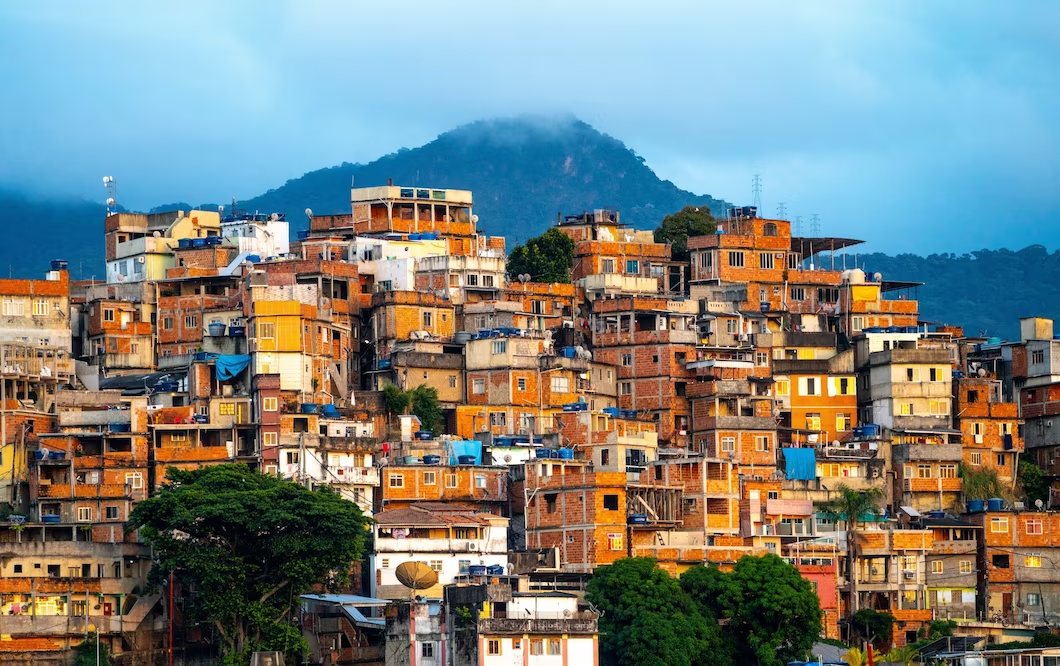
\includegraphics[width=.5\textwidth]{./imgs/img41.png}
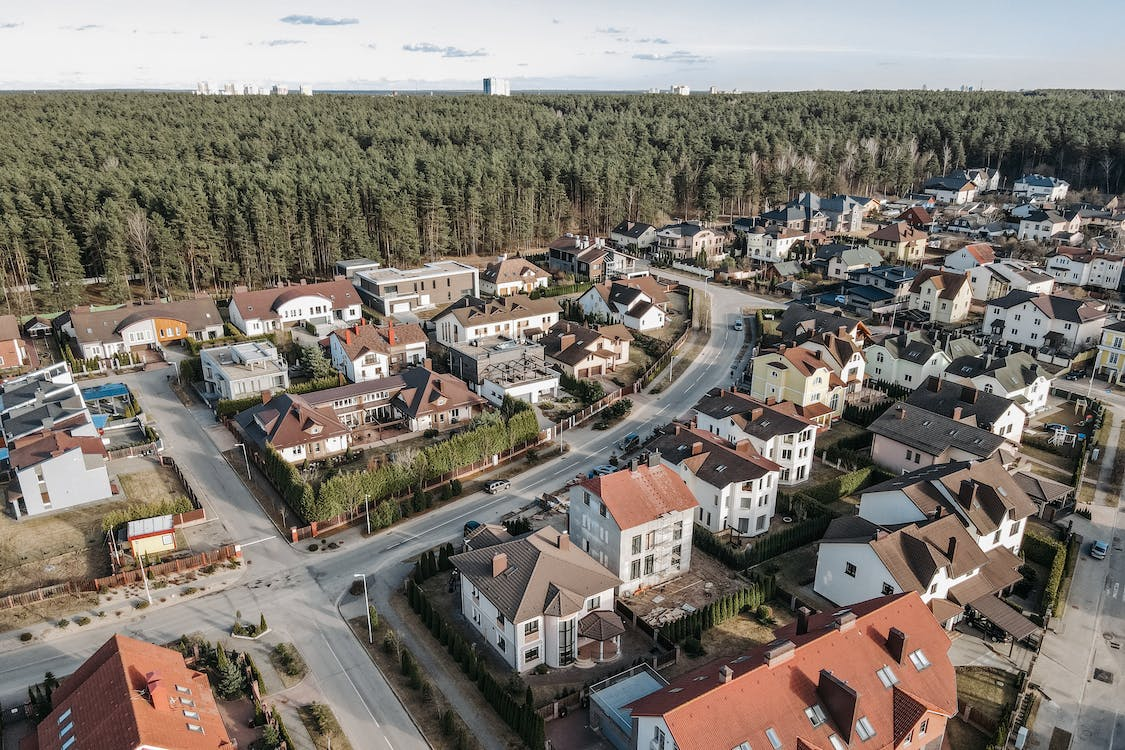
\includegraphics[width=.47\textwidth]{./imgs/img42.png}
\end{figure}

\fonte{“Morro” \emph{https://br.freepik.com/fotos-gratis/bela-vista-de-uma-pequena-cidade-nas-montanhas-durante-o-por-do-sol-no-brasil\_15695652.htm\#query=favela\&position=0\&from\_view=search\&track=sph}

“Asfalto”: \emph{https://www.pexels.com/pt-br/foto/fotografia-aerea-aerofotografia-arquitetura-tiro-com-drone-7937279/}}

\num{8} Converse com os seus colegas e com seu professor sobre as referências ao
“morro” e ao “asfalto” indicadas pelo texto 2, observe as imagens e, em
seguida, escreva as diferenças percebidas entre esses dois espaços.

\reduline{Aqui, o professor deve guiar a discussão sobre como a diferença espacial
de habitação é reveladora da diferença étnico-racial, cultural e de
classe em uma sociedade. Podem ser apontadas como diferenças: qualidade
dos edifícios, amplitude das ruas, arborização, entre outras.\hfill}
\linhas{2}

\noindent{}Vocês acham que existe uma separação de raça entre as pessoas que vivem
nos “morros” e no “asfalto” no Brasil? Discuta com seu professor e anote
os dados indicados por ele a seguir.

\begin{quote}
Porcentagem da população em morros e favelas no Brasil:

Negros: 66\%

Brancos: 34\%

Considerando a distribuição de acordo com o chefe da família, tem-se que
40,1\% dessas casas são chefiadas por homens negros, 26\% por mulheres
negras, 21,3\% por homens brancos e 11,7\% por mulheres brancas.
\end{quote}

\num{9} Segundo o texto, quando os negros saem de morros e favelas para viverem nas
moradias construídas pelo Projeto Integrado Entrada da Cidade (Piec), a
desigualdade entre brancos e negros diminui?

\reduline{Aqui, espera-se que o aluno volte ao texto e diga que não, uma vez que
os brancos ainda são colocados nas residências da frente e separados dos
negros, que em sua maioria vivem nas casas da parte de trás da Entrada
da Cidade.\hfill}

Leia o texto a seguir e responda às questões de 10 a 12.

\coment{Recomenda-se que essa atividade seja feita em duplas ou trios.}

\begin{quote}
Durante séculos, a opinião mundial se alimentou de pensamentos
distorcidos sobre a história da África, inspirados por pensadores
europeus como Friedrich Hegel, autor da frase “A África não possui
consciência exterior que possa resultar em universalidade”. A África
foi rotulada pelos europeus como uma terra sem história, por falta de
registros escritos, apesar de a escrita ter nascido no continente. {[}\ldots{}{]}

A tradição oral sempre teve um importante papel na cultura africana. A
maioria das informações culturais, sociais e ancestrais eram
transmitidas oralmente, de geração em geração. Os griôs e os mais
velhos eram, e em alguns lugares continuam sendo, os responsáveis por
essas transmissões. Como dizia o escritor Amadou Hampaté Bâ, natural de
Mali, “Na África, quando morre um velho, é toda uma biblioteca que
queima”. {[}\ldots{}{]}

Desde a antiguidade, grandes fatos históricos e grandes nomes de heróis
eram imortalizados pela música. Todo povo tinha seus griôs que conheciam
sua história de cor e a passavam para seus filhos, visto que, em geral,
ser griô era uma função hereditária. Até hoje, nos países do Sul do
Saara, é comum encontrar um jovem griô de vinte anos que consiga contar
a história de uma família por sete gerações através de uma canção
enquanto dedilha sua Kora. Além de ser o jornal da comunidade, a música
na África também sempre carregou lições de moral, já que ela é destinada
a todos. Por isso que muitas músicas tradicionais eram até histórias do
dia a dia (storytelling) que findavam com um ensinamento. {[}\ldots{}{]}

\fonte{Da Redação. Mundo Negro. A importância da tradição oral africana para a manutenção da história. Disponível em:
\emph{https://mundonegro.inf.br/a-importancia-da-tradicao-oral-africana-para-a-manutencao-da-historia/}.
Acesso em: 23 fev. 2023.}
\end{quote}

\num{10} Segundo o texto, qual é a importância da oralidade para os povos africanos?

\reduline{Espera-se que os alunos falem sobre a importância da oralidade na garantia
da perpetuação da cultura, da história e dos costumes dos povos
africanos desde a antiguidade.\hfill}
\linhas{1}

\num{11} Segundo o que vocês leram, o que é história oral?

\reduline{Aqui, espera-se que os alunos diferenciem a história oral da história
escrita, entendendo ambas como igualmente relevantes. Deve-se destacar o
processo da oralidade, da comunicação direta e da passagem de
informações através de gerações.\hfill}
\linhas{2}

\pagebreak
\num{12} Citem dois tipos de história oral presentes no texto.

\begin{enumerate}
\item \reduline{Contar histórias - griô\hfill}

\item \reduline{Músicas\hfill}
\end{enumerate}


\coment{Vale a pena, ao final das atividades, comentar alguns pontos essenciais com os alunos.
1. A África é um continente múltiplo, e não deve ser considerada uma só.
  Possui incontáveis povos e etnias, cuja história varia entre a origem
  da escrita pelos egípcios até as histórias orais de diversas
  comunidades.
2. Existem organizações sociais - complexas ou não - espalhadas pelo
  território. Existem funções sociais desempenhadas em famílias de
  maneira hereditária há muitas gerações, como a do Griô.
3. A cultura é extremamente rica, a exemplo das músicas tradicionais
  também passadas por gerações, além de outros exemplos de culturas
  materiais e imateriais.}

\colorsec{Treino}

\num{1}

\begin{quote}
{[}\ldots{}{]} Os dados indicam que a Covid-19 tem sido mais letal entre os negros
do que entre os brancos. Um ponto de partida essencial para debater essa
vulnerabilidade maior é reconhecer a desigualdade estrutural presente na
sociedade brasileira. Levantamento do IBGE, de 2018, mostra que 75\% dos
mais pobres no país são negros. Sabemos que um dos pressupostos para a
não contaminação pelo coronavírus é conseguir fazer o isolamento social.
Só que sabemos também que as condições para que esse isolamento ocorra
não são iguais para todos. Sabemos que a Covid desorganizou de maneira
bastante intensa a economia, o país de modo em geral, uma vez que muitas
pessoas não tinham trabalho formal, viviam na informalidade, ou com os
próprios negócios, ou com bicos e trabalhos que não eram fixos. Com a
falta de renda para se manterem em casa, as pessoas precisam sair para
trabalhar e, muitas vezes, se contaminam e morrem mais. {[}\ldots{}{]} 

\fonte{Andréa Vilhena. Centro de Estudos Estratégicos da Fiocruz Antonio Ivo de Carvalho. Pandemia torna mais explícita desigualdade étnico-racial no Brasil e moradores de favela se organizam coletivamente para sobreviver. Disponível em:
\emph{https://cee.fiocruz.br/?q=desigualdade-etnico-racial-no-Brasil-entrevista-Palloma-Menezes}.
Acesso em: 23 fev. 2023.}
\end{quote}

Segundo o texto, a pandemia do Covid-19 foi pior para os negros do que
entre os brancos por causa da (do)

\begin{escolha}
\item localização de seus bairros residenciais.

\item diferença em suas condições financeiras.

\item cultura de higienização das mãos.

\item mudança de seus hábitos alimentares.
\end{escolha}

\coment{BNCC: EF05GE02 - Identificar diferenças étnico-raciais e étnico-culturais e
desigualdades sociais entre grupos em diferentes territórios.}

\num{2}

\begin{quote}
A Ágora era o nome que se dava, na Grécia Antiga, às praças públicas. Nelas, ocorriam reuniões nas quais se discutiam assuntos importantes para as cidades e suas populações. No mundo moderno, esses espaços deram origem aos espaços públicos, os quais, em teoria, podem e devem ser ocupados por todos. 
A denominação muda, mas a essência continua. Fpi com os gregos que surgiu esse conceito do espaço de todos, em que há liberdade para a filosofia, o comércio, as tribunas populares.
\end{quote}

\begin{figure}[htpb!]
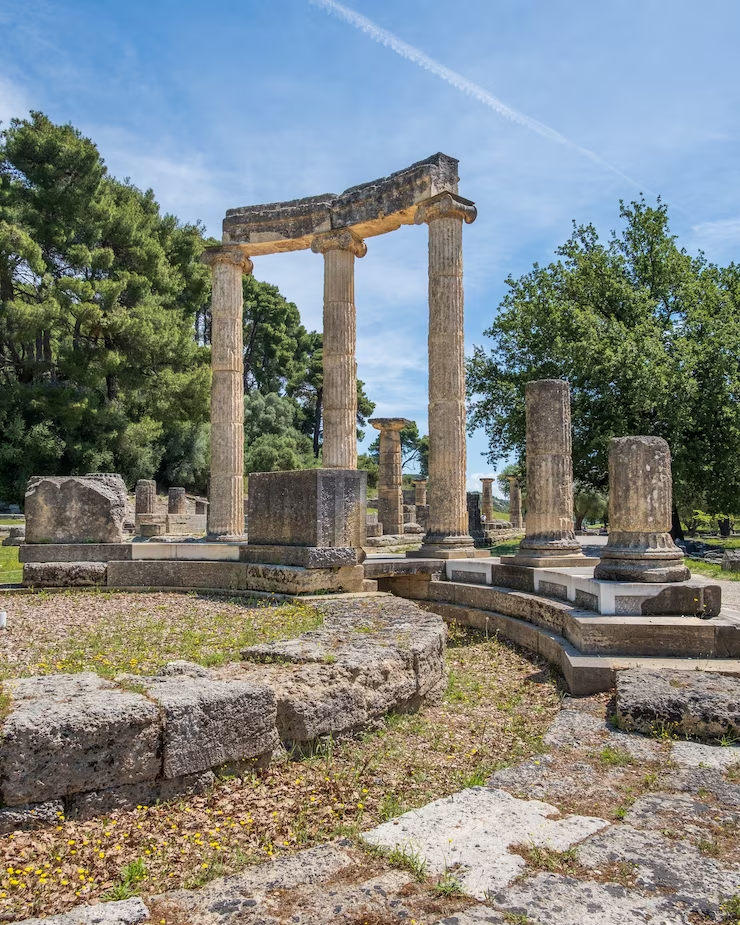
\includegraphics[width=.5\textwidth]{./imgs/img43.png}
\caption{}
\end{figure}

\noindent{}Segundo o texto, a Ágora foi um importante espaço criado pela cultura
grega onde aconteciam

\begin{minipage}{.5\textwidth}
\begin{escolha}
\item colheitas de plantações.

\item debates entre os cidadãos.

\item rituais de cunho religioso.

\item combates entre as cidades.
\end{escolha}
\end{minipage}
\sidetext{BNCC: EF05HI03 - Analisar o papel das culturas e das religiões na composição
identitária dos povos antigos.}

\num{3}

\begin{figure}[htpb!]
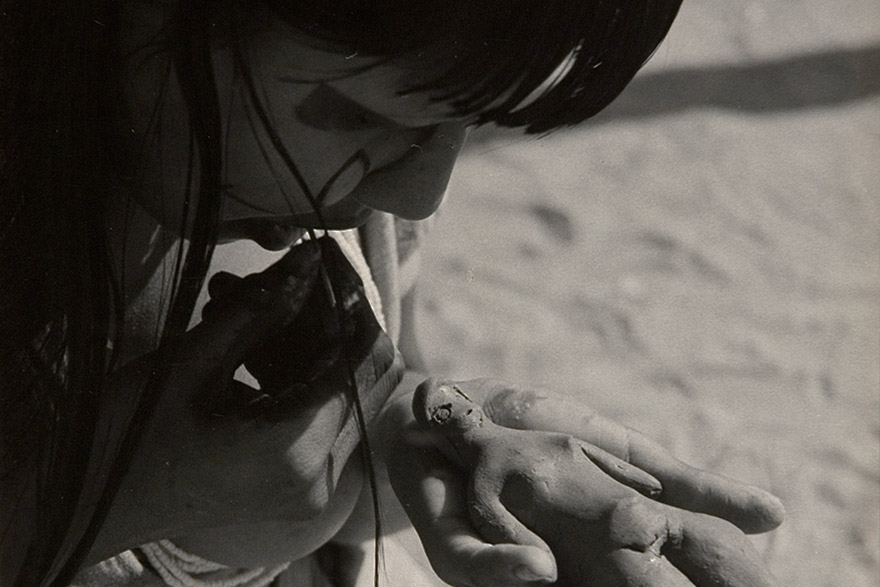
\includegraphics[width=.5\textwidth]{./imgs/img44.png}
%\caption{Imagem: Reprodução IPHAN: \emph{http://portal.iphan.gov.br/pagina/detalhes/81/}}
\end{figure}

\begin{quote}
A feitura das bonecas Karajá representa uma referência cultural significativa para o povo Karajá, além de ser, muitas vezes, a principal - ou única - fonte de renda de famílias. Nos dias atuais, a confecção dessas bonecas é feita exclusivamente por mulheres e esses saberes são transmitidos de geração em geração. Mais do que objetos meramente lúdicos, trata-se de representações culturais que carregam simbologias e significados profundos.
\end{quote}

Segundo o texto, o Modo de Fazer Bonecas Karajá é importante para o povo
Karajá por dois motivos:

\begin{minipage}{.5\textwidth}
\begin{escolha}
\item ambiental e religioso.

\item político e alimentar.

\item escolar e comportamental.

\item financeiro e cultural.
\end{escolha}
\end{minipage}
\sidetext{BNCC: EF05HI10 - Inventariar os patrimônios materiais e imateriais da
humanidade e analisar mudanças e permanências desses patrimônios ao
longo do tempo.}

\chapter{Organizações e instituições}
\markboth{Módulo 4}{}

\coment{Habilidade da BNCC: EF05HI02.}

\colorsec{Eixo de conhecimento do SAEB}

\begin{itemize}
\item Poder, estado e instituições.
\end{itemize}


\conteudo{Como nossa sociedade é organizada? Quem toma conta dela? Como chegamos
a esse sistema? Desde o surgimento da raça humana tentamos nos organizar
para viver de forma mais prática e segura. Juntamo-nos para nos
proteger contra os animais; depois, para cultivarmos nosso alimento; em
seguida, para crescer enquanto povo, até formarmos cidades, estados e
países. Chegamos à organização do nosso mundo de hoje a partir de nossa
história enquanto povo, enquanto humanidade.

\begin{wrapfigure}{l}{.5\textwidth}
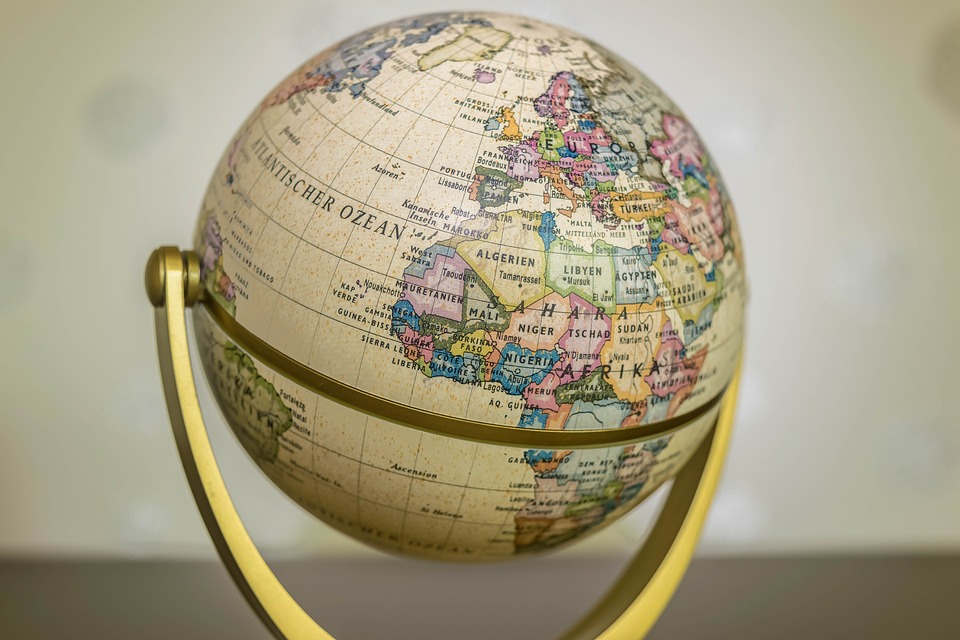
\includegraphics[width=.48\textwidth]{./imgs/img45.png}
\end{wrapfigure}
%\fonte{Disponível em: \emph{https://pixabay.com/pt/photos/globo-terra-mapa-do-mundo-mundo-1130870/} Acesso em: 23 fev. 2023.}

Hoje, o mundo se divide em 6 continentes, divididos em 193 países. Cada
país tem sua própria forma de organização. O Estado brasileiro, por
exemplo, em que vivemos, tem sua Constituição, um conjunto de leis que
temos que seguir para vivermos em nossa sociedade. Ao mesmo tempo
existem organizações internacionais, como a ONU, ou a Organização das
Nações Unidas, que trabalham para a paz entre os países e pela garantia
dos direitos humanos a todos. Temos também, dentro do Brasil, diversas
organizações - do governo ou independentes - que trabalham em benefício do
bem-estar social em diversas áreas: ambiental, cultural, social, entre
muitas outras.

Neste módulo, vamos estudar as formas de organização de nossa sociedade,
as instituições que cuidam dela e as disputas que existem entre os
vários tipos de poder social.}\pagebreak

\colorsec{Atividades}

\begin{figure}[htpb!]
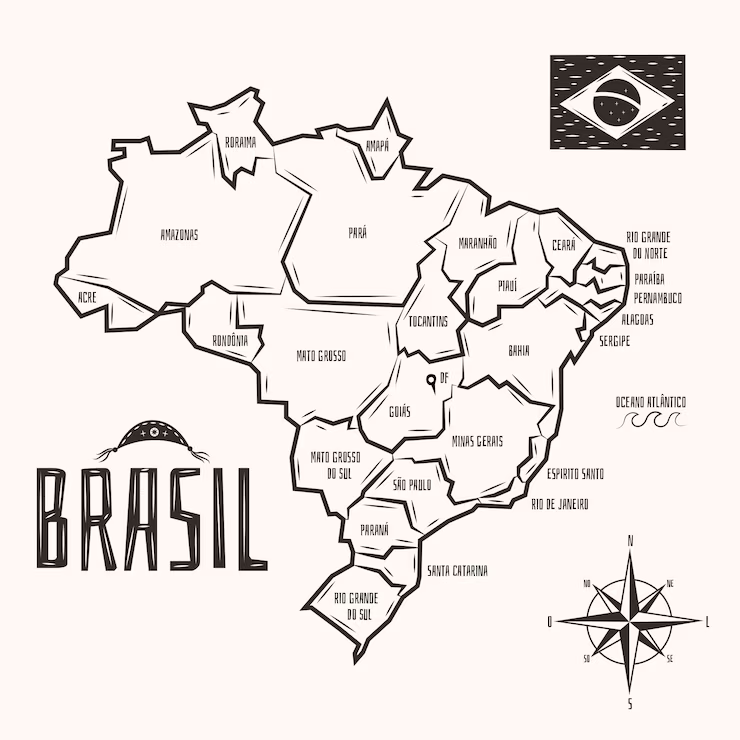
\includegraphics[width=\textwidth]{./imgs/img46.png}
\caption{}
\end{figure}

\begin{quote}
{[}...{]} O Brasil é uma República Federativa organizada política e
administrativamente em estados, municípios e distritos. Para administrar
o país, existe uma divisão em governos: federal, estadual e municipal.

Os 26 estados brasileiros, além do Distrito Federal, compõem a República
Federativa do Brasil. Por isso, os estados são chamados de Unidades da
Federação.

A sede do governo brasileiro fica em Brasília, no Distrito Federal. É lá
que trabalha o Presidente da República. {[}\ldots{}{]}

\fonte{IBGE Educa. Nosso território. Disponível em:
\emph{https://educa.ibge.gov.br/criancas/brasil/nosso-territorio/19637-divisao-territorial.html}.
Acesso em: 23 fev. 2023.}
\end{quote}\pagebreak

\noindent{}Observe o mapa, leia o texto e responda às questões a seguir.

\num{1} Você sabe o que significa a divisão dos governos em Federal, Estadual e
Municipal? Com a ajuda de seu professor, preencha os governos que tomam
conta de onde você mora.

\begin{itemize}
\item Governo Federal: \reduline{Brasil.\hfill}

\item Governo Estadual: \reduline{preencher com o Estado em que o aluno mora.\hfill}

\item Governo Municipal: \reduline{preencher com a cidade em que o aluno mora.\hfill}
\end{itemize}

\num{2} Agora, marque o estado em que você mora com um X no mapa acima.

\coment{Oriente os alunos sobre onde devem localizar o estado em que os alunos vivem.}

\num{3} Você sabia que os Estados Brasileiros são divididos em 5 regiões? Com a
ajuda do seu professor e de seus colegas, pinte com 5 cores diferentes os estados que pertencem a cada região do Brasil; depois,
anote a seguir.

\begin{itemize}
\item Região Norte:
\reduline{Amazonas, Roraima, Amapá, Pará, Tocantins, Rondônia, Acre.\hfill}
\linhas{1}

\item Região Nordeste:
\reduline{Maranhão, Piauí, Ceará, Rio Grande do Norte, Pernambuco, Paraíba, Sergipe, Alagoas, Bahia.\hfill}

\item Região Centro-Oeste:
\reduline{Mato Grosso, Mato Grosso do Sul, Goiás, Distrito Federal.\hfill}
\linhas{1}

\item Região Sudeste:
\reduline{São Paulo, Rio de Janeiro, Minas Gerais e Espírito Santo.\hfill}
\linhas{1}

\item Região Sul:
\reduline{Paraná, Santa Catarina e Rio Grande do Sul.\hfill}
\linhas{1}

\item Em qual região você mora?
\reduline{Preencher com a região onde o aluno mora.\hfill}
\linhas{1}
\end{itemize}

\pagebreak
\num{4} Você sabe para que serve essa divisão em regiões? Registre abaixo as
explicações de seu professor.

\begin{mdframed}[linewidth=2pt,linecolor=salmao]
\coment{Explicar aos alunos sobre a aplicabilidade das regiões: 
“O Brasil é um
país muito grande e de Norte a Sul encontramos costumes muito
diferentes. As danças populares são típicas de cada lugar, assim como a
comida, as músicas, as atividades econômicas e às vezes a própria língua
é tão diferente que não entendemos muito bem o que dizem as pessoas de
outras regiões. Então, para melhor compreender, estudar e administrar
este nosso imenso país, o território foi dividido em cinco grandes
regiões: Norte, Nordeste, Sul, Sudeste e Centro-Oeste. {[}...{]}”}
\end{mdframed}

\fonte{IBGE Educa. Nosso território. Disponível em:
\emph{https://educa.ibge.gov.br/criancas/brasil/nosso-territorio/19637-divisao-territorial.html}. Acesso em: 23 mar. 2023.}

\begin{figure}[htpb!]
\centering
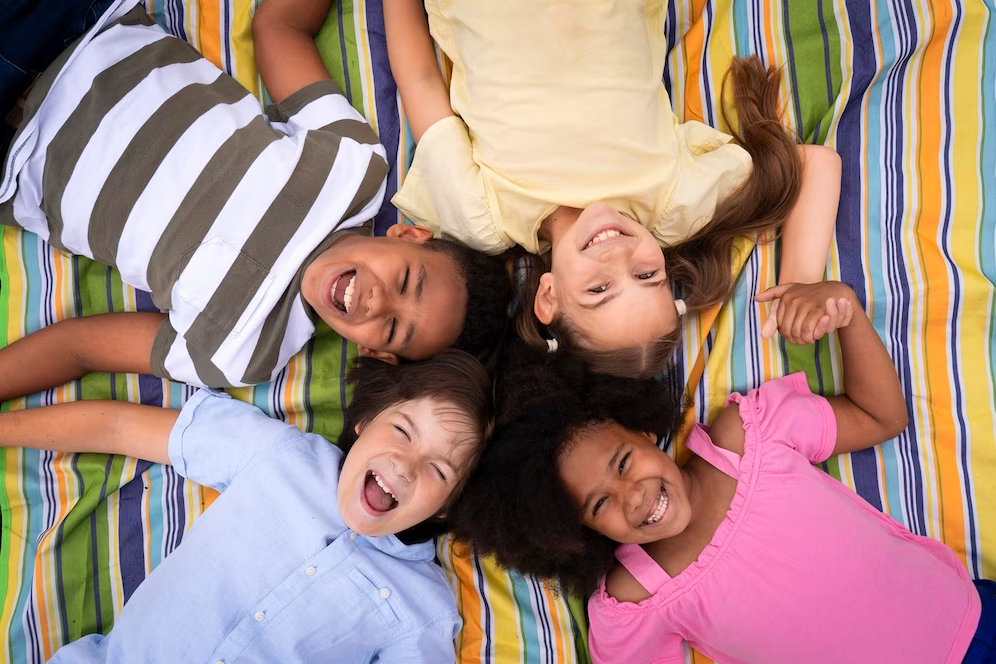
\includegraphics[width=.5\textwidth]{./imgs/img47.png}
\end{figure}
\fonte{Disponível em: \emph{https://br.freepik.com/fotos-gratis/filhos-de-tiro-medio-deitados-juntos\_17808648.htm\#query=crian\%C3\%A7a\%20lazer\&position=25\&from\_view=search\&track=ais} Acesso em: 23 fev. 2023.}

\noindent{}Você sabia que é dever do Estado brasileiro proteger as crianças e
adolescentes que vivem aqui? Para isso, foi criado o ECA,
\textbf{Estatuto da Criança e do Adolescente.} Nele estão escritos
alguns direitos que devem ser garantidos pelo governo. Vamos ler 5
deles para responder às questões que aparecem em seguida.

\begin{enumerate}[label=\textcolor{blue}{\arabic*.}]
\item Direito à liberdade, ao respeito e à dignidade: O direito à
liberdade da criança compreende que tenham o direito de ir, vir e estar
em espaços públicos e comunitários, com exceção das restrições legais. O
direito de opinião e expressão, de crença, de brincar, de praticar
esportes e se divertir, de ter refúgio, auxílio e orientação, de
participar da vida familiar e comunitária sem discriminação;

\item Ser protegido da violência física ou psicológica: {[}\ldots{}{]} crianças e adolescentes devem ter a integridade física, moral
e psíquica preservadas. Incluindo a preservação da imagem, identidade,
autonomia, ideias, crenças, valores, espaços e objetos pessoais. É ainda
dever de toda sociedade zelar pela dignidade das crianças e
adolescentes, protegendo de quaisquer tratamentos desumanos, violentos
ou constrangedores;

\item Direito à convivência familiar e comunitária: É direito da criança
ser educada pela sua família; excepcionalmente, por uma família adotiva.
Em ambiente em que esteja garantido o seu desenvolvimento integral;

\item Direito a educação, esporte e lazer: Toda criança e adolescente tem
direito à educação, para o seu desenvolvimento pessoal, qualificação
para o trabalho e preparo para o exercício da cidadania. Este direito
deve garantir que tenham condições de acesso e permanência igualitários
na escola, que sejam respeitados pelos seus educadores, que possam
contestar critérios de avaliação, podendo se expressar e recorrer às
instâncias escolares. O ECA ainda assegura o direito de participação em
entidades estudantis e o acesso à escola pública e gratuita próxima da
sua residência;

\item Direito à profissionalização e à proteção no trabalho: É proibido
qualquer trabalho a menores de quatorze anos de idade, exceto na
condição de aprendiz. A formação técnico-profissional deve obedecer às
seguintes regras: garantia de acesso e frequência obrigatória ao ensino
regular, atividade compatível com desenvolvimento do adolescente e
horário especial para o exercício do trabalho. {[}\ldots{}{]}
\end{enumerate}

\fonte{Câmara municipal de São Paulo. Mês das crianças: conheça 5 direitos de crianças e adolescentes. Disponível em:
\emph{https://www.saopaulo.sp.leg.br/blog/mes-das-criancas-conheca-5-direitos-de-criancas-e-adolescentes/\#:\textasciitilde{}:text=Garantir\%20que\%20todas\%20as\%20crian\%C3\%A7as,Poder\%20P\%C3\%BAblico\%2C\%20mas\%20de\%20toda}.
Acesso em: 23 fev. 2023.}

\num{5} Você conhecia todos esses direitos? Tem algum deles que você ache mais
importante? Existe algum direito fundamental que você acrescentaria a
esses 5 direitos? Converse com os colegas e anote suas ideias a seguir.

\reduline{Espera-se que o aluno reflita sobre os direitos lidos. Também se espera que ele
entenda suas importâncias e tenha um pensamento crítico sobre essa
questão. Além disso, a ideia é que as reflexões sejam propositivas, ao acrescentar algo que o aluno acredite faltar no conteúdo do texto lido.\hfill}
\linhas{4}

\num{6} Na sua opinião, quem é responsável pela sua educação e pelo seu
bem-estar? Discuta com seus colegas.

\reduline{Espera-se que o aluno fale sobre a família, a escola e o governo. Cabe
ao professor guiar o debate e lembrar de todas as instâncias
responsáveis por cuidar das crianças e dos adolescentes.\hfill}
\linhas{1}

\num{7} Você sabia que existe uma lei que responde a esta questão? Copie da
lousa essa lei no retângulo a seguir.

\begin{mdframed}[linewidth=2pt,linecolor=salmao]
\coment{Art. 227. É dever da família, da sociedade e do Estado assegurar à
criança e ao adolescente, com absoluta prioridade, o direito à vida, à
saúde, à alimentação, à educação, ao lazer, à profissionalização, à
cultura, à dignidade, ao respeito, à liberdade e à convivência familiar
e comunitária, além de colocá-los a salvo de toda forma de negligência,
discriminação, exploração, violência, crueldade e opressão.}
\end{mdframed}

\fonte{Governo do estado do Paraná. Constituição Federal. Disponível em:
\emph{https://www.justica.pr.gov.br/Pagina/Constituicao-Federal}.
Acesso em: 23 mar. 2023.}

\num{8} Você sabia da existência do Estatuto da Criança e do Adolescente? Por que
você acha que ele é importante em nossa sociedade? Discuta com o
professor e seus colegas e escreva a seguir.

\reduline{Falar sobre a responsabilidade do Poder Público, e não só da família, de
proteger as crianças. Discutir o conceito de direito: o que é? Quem
trabalha para que ele seja garantido? Falar sobre a importância da
existência de um órgão do governo que tenha como objetivo criar
políticas públicas em prol das crianças e dos adolescentes.\hfill}

\num{9} Você sabe até quantos anos uma pessoa é considerada criança pelo ECA? E
adolescente? Complete com a ajuda do professor:

\begin{itemize}
\item Criança: De \reduline{zero} até \reduline{doze} anos de idade.

\item Adolescente: Entre \reduline{doze} e \reduline{dezoito} anos de idade.
\end{itemize}

\conteudo{Agora já sabemos quem são os responsáveis por cuidar das crianças e
adolescentes. Os pais, a família, a escola e o estado têm esse dever.

Mas quais são os deveres das crianças e dos adolescentes na comunidade?

Na próxima atividade falaremos sobre as regras de convivência na escola.}

\coment{Recomenda-se que as atividades sejam feitas em duplas ou grupos, para
que não se torne extremamente séria ou acusativa. O objetivo é que os
alunos discutam sobre as regras de maneira leve e natural.}

Vamos começar lendo uma parte de uma reportagem de 2018. Depois, vamos responder às questões de 10 a 12.

\begin{quote}
\textbf{Cotidiano: a importância das normas de convivência para o bem-estar na escola}\\
Quando a criança aprende a respeitar o direito do outro, entra em
contato com o conceito de ética logo na infância.

Conviver é um exercício diário de cidadania. Viver em sociedade é, acima
de tudo, uma necessidade humana. {[}\ldots{}{]} Esse exercício social se inclina,
principalmente, ao respeito, às diferenças e ao ato de obedecer às
regras de conduta moral e ética. Para as crianças, em especial, as
normas de relacionamento com o meio são mais bem exercidas na escola,
onde o ato de dividir o mesmo espaço é mais intenso. {[}\ldots{}{]}

\fonte{ G1. Cotidiano: a importância das normas de convivência para o bem-estar na escola. Disponível em:
\emph{https://g1.globo.com/sao-paulo/sorocaba-jundiai/especial-publicitario/objetivo-sorocaba/conduzindo-o-melhor-de-voce/noticia/cotidiano-a-importancia-das-normas-de-convivencia-para-o-bem-estar-na-escola.ghtml}.
Acesso em: 23 fev. 2023.}
\end{quote}

\num{10} Vamos começar lembrando algumas \textbf{regras gerais} que temos em
nossa escola. Com a ajuda dos colegas, escreva 3 delas.

\begin{enumerate}[label=\textcolor{blue}{\arabic*.}]
\item \linhas{1}

\item \linhas{1}

\item \linhas{1}
\end{enumerate}

\coment{Aqui, cabe ao professor guiar a discussão dos alunos e elencar com eles
as principais regras da escola. Exemplos: chegar no horário, cuidar do
ambiente escolar, usar uniforme etc.}

\num{11} Agora, vamos falar das regras que temos que cumprir dentro da sala de
aula.

\begin{enumerate}[label=\textcolor{blue}{\arabic*.}]
\item \linhas{1}

\item \linhas{1}

\item \linhas{1}

\item \linhas{1}

\item \linhas{1}
\end{enumerate}

\coment{Aqui, cabe ao professor guiar a discussão dos alunos e elencar com eles
as principais regras a serem cumpridas dentro da sala de aula. Exemplos:
obedecer ao professor, não conversar durante a explicação, sentar no
lugar correto, anotar a matéria no caderno etc.}

\num{12} Você sabe por que as regras são importantes?

\reduline{Aqui, o professor deve guiar o aluno a entender que, assim como a escola, a família e o governo têm o dever de proteger os alunos,
os alunos também têm deveres dentro da sociedade, sendo o principal
deles permitir que a educação na escola aconteça da forma mais leve e
fácil possível. Falar também sobre a organização e sobre a importância dela no
futuro dos alunos.}
\linhas{2}

\colorsec{Treino}

\num{1}

\begin{quote}
{[}...{]} Segundo a nossa Constituição, a República Federativa do Brasil é
formada pelos Estados, Municípios e pelo Distrito Federal, que se aliam
numa união indissolúvel para a formação de um Estado Federal ou
Federação. Por isso é que a Constituição, em seu primeiro artigo,
estabelece que a organização político-administrativa da República
Federativa do Brasil abrange os Estados, o Distrito Federal, os
Municípios e a União - com U maiúsculo -, pessoa jurídica que resultou
daquela união indissolúvel, que representa a Federação. {[}\ldots{}{]}

\fonte{ Organização do estado brasileiro. Disponível em: \emph{https://dspace.almg.gov.br/}. Acesso em: 23 fev. 2023.}
\end{quote}

Um exemplo de município é

\begin{escolha}
\item o bairro Cidade Nova, na cidade de Manaus.

\item o estado de Minas Gerais, no Sudeste.

\item a cidade de Campinas, em São Paulo.

\item a região Nordeste do Brasil.
\end{escolha}

\coment{BNCC: EF05HI02 - Identificar os mecanismos de organização do
poder político com vistas à compreensão da ideia de Estado e/ou de
outras formas de ordenação social.}

\pagebreak
\num{2}

\begin{quote}
As terras que hoje são chamadas de Brasil têm muitos nomes, atribuídos pelos
povos originários. Alguns exemplos são “Pindorama” e “Yvy Rupa”. O continente em que hoje
vivemos, chamado de América, é conhecido também por Abya Ayla, Tawantinsuyu, Anáhuac - respectivamente pelos
povos Kuna, Inca e Asteca. Com os nomes, aprendemos a importância das
coisas: dar um nome a uma região, a uma pessoa ou a um povo ajuda na identificação desses elementos. Você conhece a palavra “identidade”?
Dar nomes tem tudo a ver com identificar o mundo: as
identidades tornam as pessoas únicas, assim como seus grupos, os locais que conhecemos e os povos que vivem nesses lugares.

\fonte{Fonte de pesquisa: \emph{https://nheepora.mlp.org.br/} Acesso em: 23 fev 2023.}
\end{quote}

Segundo o texto, ao dar nome a um território estamos

\begin{minipage}{0.5\textwidth}
\begin{escolha}
\item protegendo suas florestas.

\item expressando suas características.

\item medindo seu valor econômico.

\item julgando sua beleza natural.
\end{escolha}
\end{minipage}
\sidetext{BNCC: EF05HI02 - Identificar os mecanismos de organização do
poder político com vistas à compreensão da ideia de Estado e/ou de
outras formas de ordenação social.}


\num{3}

\begin{quote}
\textbf{Estatuto da Criança e do Adolescente Lei nº 8.069, de 13 de julho de 1990}\\
Art. 7º A criança e o adolescente têm direito à proteção à vida e à
saúde, mediante a efetivação de políticas sociais públicas que permitam
o nascimento e o desenvolvimento sadio e harmonioso, em condições dignas
de existência.

\fonte{Presidência da República. Casa Civil. Subchefia para Assuntos Jurídicos. Disponível em: \emph{https://www.planalto.gov.br/ccivil\_03/leis/l8069.htm}. Acesso em: 23 mar. 2023.}
\end{quote}

Quem é responsável pela criação de políticas sociais públicas de que
fala o texto?

\begin{minipage}{0.5\textwidth}
\begin{escolha}
\item o professor.

\item a escola.

\item a família.

\item o estado.
\end{escolha}
\end{minipage}
\sidetext{BNCC: EF05HI02 - Identificar os mecanismos de organização do
poder político com vistas à compreensão da ideia de Estado e/ou de
outras formas de ordenação social.}

\chapter{Cidadania e sociedade}
\markboth{Módulo 5}{}

\coment{Habilidades da BNCC: EF05HI04, EF05HI05.}

\colorsec{Eixo de conhecimento do SAEB}

\begin{itemize}
\item Cidadania, direitos humanos e movimentos sociais.
\end{itemize}

\conteudo{Você é um cidadão brasileiro. Mas você sabe o que isso significa?
Significa que, a partir do momento em que você nasce no Brasil, você
passa a fazer parte de nossa República - e tem direitos fundamentais e
deveres dentro do território nacional. Alguns desses direitos nós já
aprendemos no Módulo 4, quando estudamos o Estatuto da Criança e do
Adolescente(ECA). Porém, não são só as crianças e adolescentes que têm o
direito à vida, à liberdade, à igualdade, à segurança e à propriedade.
São todos os cidadãos brasileiros.

\begin{wrapfigure}{l}{.5\textwidth}
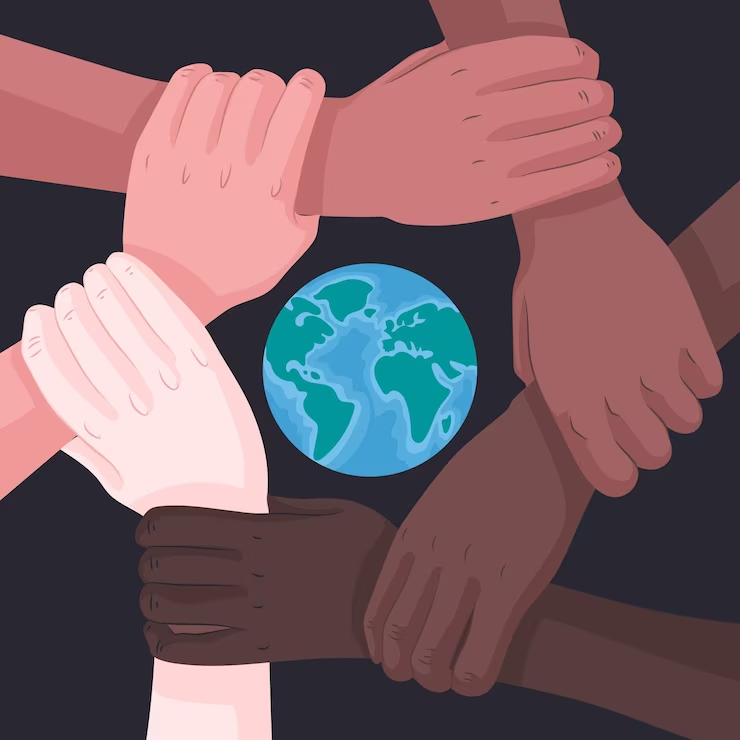
\includegraphics[width=.48\textwidth]{./imgs/img48.png}
\end{wrapfigure}

Não são só as pessoas que nascem no Brasil que têm seus direitos
garantidos. Ao longo da história foi construída a ideia de
\textbf{direitos humanos}, que são direitos que \textbf{todos os seres
humanos}, em todos os países, independentemente do que acontece no lugar em
que nasceram, devem ter. Quem trabalha para garantir esses direitos
são Órgãos internacionais, como a ONU, a Organização das Nações Unidas.

Nesse módulo vamos trabalhar o conceito de cidadania e entender nossos
direitos enquanto cidadãos brasileiros e cidadãos do mundo. Também
vamos ver como podemos lutar para que nossos direitos básicos sejam
garantidos, para que todos possam viver de maneira satisfatória e digna.

\fonte{Disponível em:
\emph{https://br.freepik.com/vetores-gratis/pare-o-conceito-de-ilustracao-de-racismo\_8944994.htm\#page=2\&query=direitos\%20humanos\&position=36\&from\_view=search\&track=ais}
Acesso em: 23 fev. 2023.}}

\colorsec{Atividades}

Vamos ler uma parte da \textbf{Declaração Universal dos Direitos Humanos}, de 1948. Depois, responder às questões 1 e 2.

\begin{quote}
{[}\ldots{}{]}
Considerando que os povos das Nações Unidas reafirmaram, na Carta, sua
fé nos direitos fundamentais do ser humano, na dignidade e no valor da
pessoa humana e na igualdade de direitos do homem e da mulher e que
decidiram promover o progresso social e melhores condições de vida em
uma liberdade mais ampla, {[}\ldots{}{]}

Agora portanto a Assembleia Geral proclama a presente Declaração
Universal dos Direitos Humanos como o ideal comum a ser atingido por
todos os povos e todas as nações, com o objetivo de que cada indivíduo e
cada órgão da sociedade, tendo sempre em mente esta Declaração,
esforce-se, por meio do ensino e da educação, por promover o respeito a
esses direitos e liberdades, e pela adoção de medidas progressivas de
caráter nacional e internacional, por assegurar o seu reconhecimento e a
sua observância universais e efetivos, tanto entre os povos dos próprios
Países-Membros quanto entre os povos dos territórios sob sua jurisdição.

\textbf{Artigo 1}

Todos os seres humanos nascem livres e iguais em dignidade e direitos.
São dotados de razão e consciência e devem agir em relação uns aos
outros com espírito de fraternidade.

\textbf{Artigo 2}

1. Todo ser humano tem capacidade para gozar os direitos e as liberdades
estabelecidos nesta Declaração, sem distinção de qualquer espécie, seja
de raça, cor, sexo, língua, religião, opinião política ou de outra
natureza, origem nacional ou social, riqueza, nascimento, ou qualquer
outra condição.

2. Não será também feita nenhuma distinção fundada na condição política,
jurídica ou internacional do país ou território a que pertença uma
pessoa, quer se trate de um território independente, sob tutela, sem
governo próprio, quer sujeito a qualquer outra limitação de soberania.

\textbf{Artigo 3}

Todo ser humano tem direito à vida, à liberdade e à segurança pessoal. {[}\ldots{}{]}

\fonte{ Unicef. Declaração Universal dos Direitos Humanos. Disponível em:
\emph{https://www.unicef.org/brazil/declaracao-universal-dos-direitos-humanos}.
Acesso em: 23 fev. 2023.}
\end{quote}

\num{1} Agora, discuta com seus colegas e marque com um X as situações
que você considera que vão \textbf{contra} os direitos humanos.

\begin{boxlist}
\boxitem{X} Ameaçar a vida de alguém. 

\boxitem{X} Torturar ou castigar alguém usando violência.

\boxitem{\white{X}} Garantir moradia a todos.

\boxitem{X} Permitir trabalho escravo e forçado.

\boxitem{\white{X}} Tratar todos de maneira igual.

\boxitem{X} Condenar alguém de maneira injusta.

\boxitem{\white{X}} Oferecer bom salário e boas condições de trabalho.

\boxitem{X} Tratar alguém de forma diferente por causa de sua cor de pele.
\end{boxlist}

\coment{É interessante comentar cada um dos itens com os alunos, frisando a importância de um a um.}

\num{2} E se você trabalhasse em um organismo internacional e tivesse que
resolver algum dos itens assinalados como problemáticos anteriormente? O que você faria?

\coment{Divida a sala em 6 grupos e atribua a esses grupos alguma das situações
sugeridas. Peça que eles pensem em soluções simples e diretas para os
problemas de ameaça aos direitos humanos. A ideia é que não seja algo
extremamente elaborado, mas que eles construam reflexões coerentes com os estudos realizados até este ponto.

Sugestões:

Grupos 1 e 2: Permitir trabalho escravo e forçado.

Grupos 3 e 4: Torturar ou castigar alguém usando violência.

Grupos 5 e 6: Tratar alguém de forma diferente por causa de sua cor de pele.}

\begin{itemize}
\item Nome: \reduline{Nome do Aluno\hfill}

\item Ano: \reduline{Ano do Aluno\hfill}

\item Nome da Organização: \reduline{Pedir aos alunos que deem um nome para o grupo. Ex:
Defensores dos direitos humanos.\hfill}

\item Integrantes: \reduline{Completar com os outros colegas do grupo.\hfill}

\item Problema: \reduline{Colocar o problema atribuído ao grupo.\hfill}

\item Propostas: \reduline{Preencher com as propostas do grupo.\hfill}
\end{itemize}

\begin{mdframed}[linewidth=10pt,linecolor=salmao,roundcorner=20pt]
\vspace{4cm}
\end{mdframed}

\noindent{}Você sabia que até o ano de 1932 as mulheres não podiam votar no Brasil?

\noindent{}Leia um texto sobre como aconteceu essa conquista. Depois, responda às questões de 3 a 5.

\begin{figure}[htpb!]
\centering
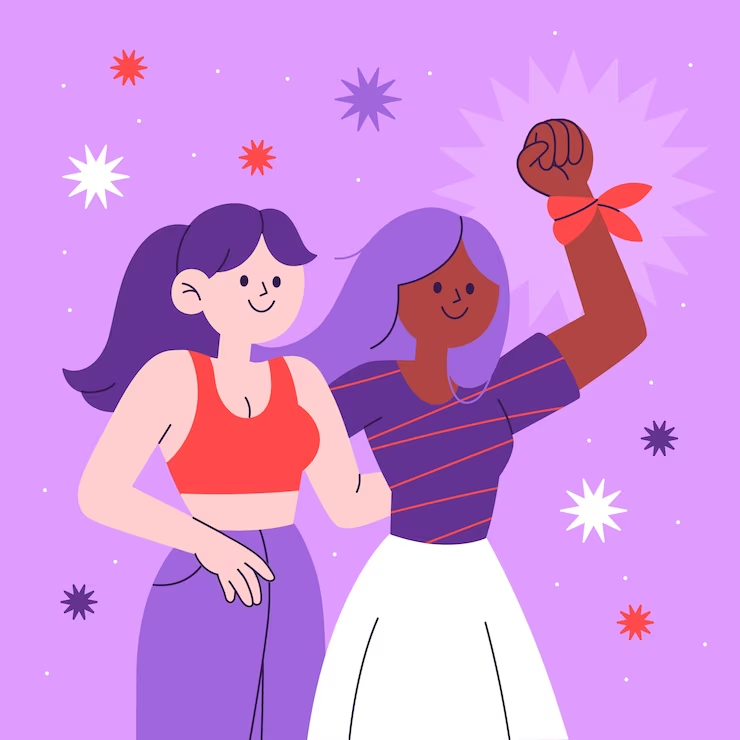
\includegraphics[width=.5\textwidth]{./imgs/img49.png}
\caption{}
\end{figure}

\begin{quote}
A conquista do voto feminino no Brasil se deu em 1932, resultado de um
processo de lutas, avanços e recuos que se iniciou por volta de 1910. {[}\ldots{}{]}

Em 1910 {[}\ldots{}{]}, a professora carioca Leolinda de Figueiredo Daltro
(1860-1935), em protesto à recusa de seu pedido de alistamento
eleitoral, fundou o Partido Republicano Feminino. Considerado o primeiro
partido político feminino do país, defendia o direito ao voto para as
mulheres e a abertura dos cargos públicos a todos os brasileiros {[}\ldots{}{]}.

Durante os trabalhos da primeira Assembleia Constituinte da República,
alguns parlamentares apresentaram propostas concretas de extensão do
direito de voto às mulheres. Lopes Trovão {[}\ldots{}{]}
 apresentou uma emenda que foi
{[}\ldots{}{]} rejeitada e a Constituição da República dos Estados Unidos do
Brasil de 1891 não contemplou as mulheres com esse direito de cidadania. {[}\ldots{}{]}
O texto da Constituição de 1891 não vedava expressamente o
direito de as mulheres votarem. Valendo-se disso, a estudante de direito
Maria Ernestina, conhecida como Mietta Santiago, {[}\ldots{}{]} obteve sentença
que lhe permitiu votar em si mesma para um mandato de deputada federal. {[}\ldots{}{]}

Em 1932 foi promulgado o novo Código Eleitoral, cuja comissão de
redação contou com a participação de Bertha Lutz. Estava assegurada a
cidadania política às mulheres brasileiras, embora sem a exigência da
obrigatoriedade do alistamento eleitoral e do voto. Os arts. 2º e 21 do
novo Código Eleitoral continham os seguintes textos:

Art. 2º. É eleitor o cidadão maior de 21 anos, sem distinção de sexo,
alistado na forma deste Código. (...)

Art. 121. Os homens maiores de sessenta anos e as mulheres de qualquer
idade podem isentar-se de qualquer obrigação ou serviço de natureza
eleitoral.

Posteriormente, a Constituição da República dos Estados Unidos do Brasil
de 1934 ratificou o direito constitucional de voto das mulheres.

\fonte{ Ricardo Oriá. Câmara dos deputados. As sufragistas: a luta pelo voto feminino. Disponível em:
\emph{https://www.camara.leg.br/internet/agencia/infograficos-html5/a-conquista-do-voto-feminino/analise.html}.
Acesso em: 23 fev 2023. (Adaptado)}
\end{quote}

\num{3} Você sabia que o voto é um direito de todos os cidadãos? Escreva qual
você acha que é a importância dele para nós.

\reduline{Aqui o professor deve guiar a discussão, primeiramente, sobre o que
significa votar (eleger uma pessoa para nos representar nas decisões
políticas e sociais de nosso país). Em segundo lugar, deve-se pensar
sobre o voto como uma escolha e expressão dos pensamentos de cada
indivíduo. Por fim, o professor deve enfatizar que o voto foi uma
conquista dos cidadãos ao longo da história, e que devemos utilizar esse
mecanismo em nosso favor.\hfill}

\num{4} Apesar de no Brasil as mulheres poderem votar desde 1932, em alguns
países isso aconteceu ainda mais tarde. Na Árábia Saudita, por exemplo,
as mulheres só podem votar desde o ano de 2011. Por que você acha que
demorou tanto tempo para as mulheres conquistarem a possibilidade de
votar no Brasil e no mundo?

\reduline{Aqui, o professor deve guiar de maneira cautelosa o debate. Falar sobre
o preconceito contra as mulheres na história da humanidade e reafirmar que, apesar
de hoje, em nossa sociedade, entendermos os homens e as mulheres como
iguais, nem sempre foi assim.\hfill}
\linhas{2}

\num{5} O voto pode ser considerado uma conquista das mulheres? Cite as
personagens que o texto aponta como importantes nesse processo e o que
elas fizeram para lutar a favor dos direitos das mulheres enquanto
cidadãs:

\reduline{Sim. É importante, neste ponto, o professor guiar o aluno a entender os conceitos de
luta e conquista de direitos humanos, sociais e políticos.\hfill}\\
\reduline{Personagens:\hfill}\\
\reduline{Leolinda de Figueiredo Daltro (1860-1935): em protesto à recusa de seu
pedido de alistamento eleitoral, fundou o Partido Republicano Feminino.\hfill}\\
\reduline{Mietta Santiago: obteve sentença que lhe permitiu votar em si
mesma para um mandato de deputada federal.\hfill}\\
\reduline{Bertha Lutz: ajudou a escrever o Código eleitoral de 1932.\hfill}

\begin{figure}[htpb!]

\includegraphics[width=.5\textwidth]{./imgs/img50.png}
\end{figure}
\fonte{Disponível em: \emph{https://br.freepik.com/fotos-gratis/pile-of-3d-twitter-logos\_1191372.htm\#query=twitter\&position=9\&from\_view=search\&track=sph} Acesso em: 23 fev. 2023.}

Leia um texto sobre a rede social Twitter para, então, responder às questões que seguem.

\begin{quote}
\textbf{Desaparecimento do Twitter seria má notícia para ativistas
políticos, dizem analistas }

{[}\ldots{}{]}
Existem outras plataformas, mas o Twitter “é claramente muito influente
ao fazer com que a mídia e os líderes prestem atenção no que acontece no
mundo”, disse à AFP Mahsa Alimardani, pesquisadora da organização de
defesa da liberdade de expressão Artigo 19.

– Nesse sentido, é uma plataforma única e muito especial –
acrescenta. – {[}No Irã{]} é o único acesso real a vozes e eventos, na
ausência de correspondentes estrangeiros e jornalistas independentes que
possam informar sobre o que está acontecendo. {[}\ldots{}{]}

O Twitter tem desempenhado um papel fundamental na promoção de fenômenos
sociais como o \#Metoo (eu também), para denunciar a violência contra a
mulher, ou o \#Blacklivesmatter (Vidas negras importam), para denunciar
a violência policial contra negros nos Estados Unidos.

– As características do Twitter permitem dar uma identidade aos
movimentos de protesto, criar um sentimento comum ao compartilhar memes
e hashtags – explicou à AFP Marcus Michaelsen, pesquisador independente especializado em ativismo e vigilância on-line. {[}\ldots{}{]}

\fonte{O Globo. Mundo. Disponível em:
\emph{https://oglobo.globo.com/mundo/noticia/2022/11/desaparecimento-do-twitter-seria-ma-noticia-para-ativistas-politicos-dizem-analistas.ghtml}.
Acesso em: 23 fev. 2023.}
\end{quote}

\num{6} Você sabe o que é uma rede social? Cite as que você conhece.

\reduline{Falar sobre redes sociais como comunidades on-line onde ocorrem trocas
entre pessoas. Os alunos ficam livres para citar as que conhecem:
Instagram, Facebook, Twitter, Tiktok etc.\hfill}
\linhas{3}

\num{7} Você acha que as redes sociais podem ajudar na luta por nossos direitos? Como?

\reduline{Aqui, volte ao texto e descreva como ele narra a importância do twitter
como plataforma de visibilidade, debate e troca entre as pessoas.\hfill}
\linhas{2}

\num{8} Cite dois exemplos de situações que o texto mostra nas quais o twitter ajudou
em movimentos sociais.

\begin{enumerate}
\item \reduline{Movimento “vidas negras importam”, para denunciar a violência policial
  contra a comunidade negra.\hfill}

\item \reduline{“Eu também”, de combate à violência contra a mulher.\hfill}
\end{enumerate}

\pagebreak
\num{9} Seu post na rede social.

Se você pudesse acabar com qualquer injustiça no mundo, qual seria?
Escreva um post para uma rede social em que você explique o que faria para ajudar nessa luta.

\begin{mdframed}[linewidth=2pt,linecolor=salmao]
\coment{Aqui, o aluno deve exercitar sua criatividade.}
\vspace{10cm}
\end{mdframed}

\num{10} Você acha que existe uma idade mínima para as pessoas estarem nas redes sociais e participarem delas? Por quê?

\reduline{A resposta é pessoal. Trata-se de excelente oportunidade para abrir discussão acerca desse delicado assunto.\hfill}
\linhas{6}

\colorsec{Treino}

\num{1}

\begin{figure}[htpb!]
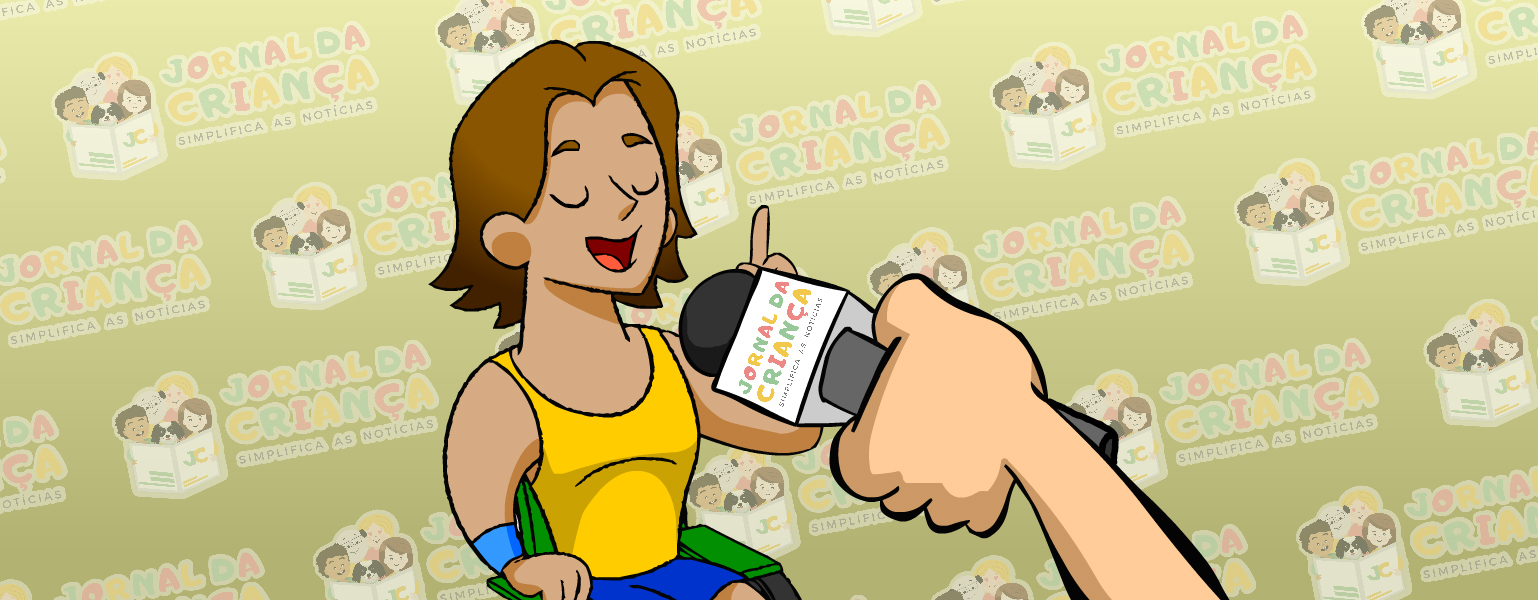
\includegraphics[width=.5\textwidth]{./imgs/img51.png}
\end{figure}

Leia um texto em que o personagem Vital, do Plenarinho, da Câmara dos Deputados, dá uma entrevista ao Jornal da Criança.

\begin{quote}
\textbf{Vital, qual é a importância do voto?}

Votar quer dizer declarar a nossa escolha entre duas ou mais opções.
Falando assim, parece uma coisa simples, né? Mas, quando se trata de
eleições, votar é um assunto muito sério. É escolher entre as propostas
de futuro que a gente quer para a nossa comunidade, o nosso estado, o
nosso país!

\noindent\textbf{Nossa, voto é assunto sério, mesmo!}

Com certeza! Quando o eleitor vota em um representante – deputado,
senador, governador, presidente -, é como se dissesse: “estou confiando
em você para falar em meu nome e tomar por mim todas as decisões
importantes do País”. Não dá para fazer essa escolha sem pensar bem,
né?

\fonte{Câmara dos Deputados. Plenarinho. A turma explica as eleições - qual a importância do voto? Disponível em:
\emph{https://plenarinho.leg.br/index.php/2022/09/turma-explica-eleicoes-qual-importancia-voto/}.
Acesso em: 23 fev. 2023.}
\end{quote}

Segundo Vital, ao votar estamos

\begin{minipage}{0.5\textwidth}
\begin{escolha}
\item escolhendo o futuro do país.

\item decidindo nossa profissão.

\item disfarçando nossos erros.

\item cuidando da saúde do nosso corpo.
\end{escolha}
\end{minipage}
\sidetext{BNCC: EF05HI04 - Associar a noção de cidadania com os
princípios de respeito à diversidade, à pluralidade e aos direitos
humanos.}


\num{2}

\begin{quote}
\textbf{Crianças indígenas defendem demarcação de terra e autonomia
sobre territórios}

{[}\ldots{}{]}
Brincar perto da natureza, ter uma casa para morar, manter os costumes
da sua família, ir para a escola e viver em segurança são direitos de
todas as crianças, mas em algumas terras indígenas eles estão ameaçados.
Isso ocorre porque esses territórios são invadidos por pessoas e
empresas que querem explorar a natureza e expulsar os indígenas. {[}\ldots{}{]} 
A luta
tem conquistado cada vez mais apoiadores graças a muitos jovens
indígenas que se tornaram influencers e usam o youtube, o instagram e
outras redes sociais para falar sobre sua cultura, suas reivindicações e
também sobre música, literatura, jogos online e diversos outros
assuntos. {[}\ldots{}{]}

\fonte{Da Redação. Brasil de Fato. Disponível em:
\emph{https://www.brasildefato.com.br/2022/04/20/criancas-indigenas-defendem-demarcacao-de-terra-e-autonomia-sobre-territorios}.
Acesso em: 23 fev. 2023.}
\end{quote}

Segundo o texto, os jovens indígenas usam as redes sociais para

\begin{minipage}{0.5\textwidth}
\begin{escolha}
\item ganhar dinheiro com publicações\\ pagas.

\item prejudicar aqueles que tentam ameaçar seus direitos.

\item mostrar aos outros sua cultura e suas lutas.

\item pedir a separação do Brasil.
\end{escolha}
\end{minipage}
\sidetext{BNCC: EF05HI05 - Associar o conceito de cidadania à conquista
de direitos dos povos e das sociedades, compreendendo-o como conquista
histórica.}


\num{3}

\begin{figure}[htpb!]
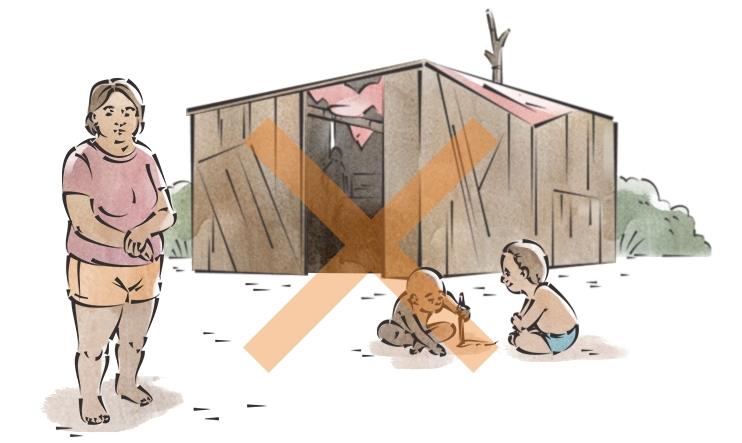
\includegraphics[width=.5\textwidth]{./imgs/img52.jpg}
\end{figure}

\noindent{}Uma medida direta que pode ser tomada pelo governo para melhorar o
acesso à moradia é

\begin{escolha}
\item a construção de habitações populares.

\item a igualdade salarial entre homens e mulheres.

\item o aumento da segurança em locais públicos.

\item a distribuição de alimentos nas comunidades.
\end{escolha}

\coment{BNCC: EF05HI04 - Associar a noção de cidadania com os
princípios de respeito à diversidade, à pluralidade e aos direitos
humanos.}

\chapter{Produção e trabalho}
\markboth{Módulo 6}{}

\coment{Habilidade da BNCC: EF05GE05.}

\colorsec{Eixo de conhecimento do SAEB}

\begin{itemize}
\item Relações de trabalho, produção e circulação.
\end{itemize}

%\fonte{Disponível em: \emph{https://br.freepik.com/fotos-gratis/um-agricultor-que-esta-usando-uma-pa-para-cavar-o-solo-em-seus-campos-de-arroz\_5491642.htm\#query=trabalho\%20terra\&position=16\&from\_view=search\&track=ais} Acesso em: 23 fev. 2023.}
%\fonte{Disponível em: \emph{https://br.freepik.com/fotos-gratis/mulher-de-close-up-costurando-com-maquina\_12810036.htm\#query=trabalho\%20costura\&position=18\&from\_view=search\&track=ais} Acesso em: 23 fev. 2023.}

\conteudo{Vocês conhecem os diferentes tipos de trabalho que existem no Brasil e
no mundo? E como eles impactam em como nós vivemos, no que comemos, no
que fazemos? Tudo o que temos e consumimos no nosso dia a dia vem do
trabalho de alguém. O arroz e feijão que comemos todos os dias foi
plantado e colhido por um trabalhador do campo, transportado por
outro trabalhador, separado e vendido no mercado onde trabalham muitas
outras pessoas. A roupa que utilizamos também foi costurada por um
trabalhador. Em seguida, foi levada a um centro comercial, onde nossos
pais compraram com a ajuda de um vendedor.

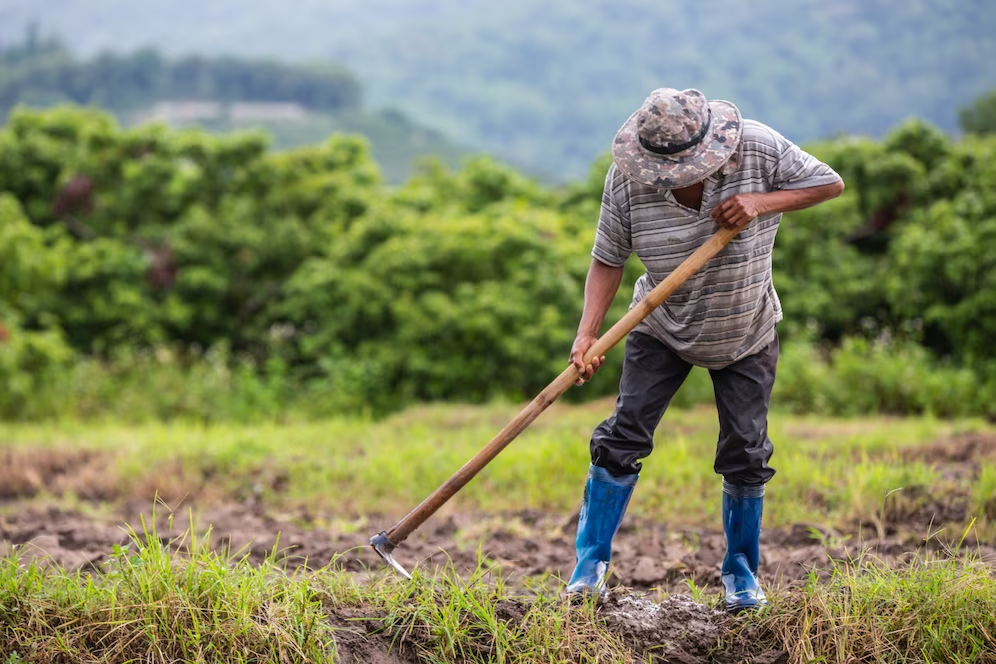
\includegraphics[width=.5\textwidth]{./imgs/img53.png}
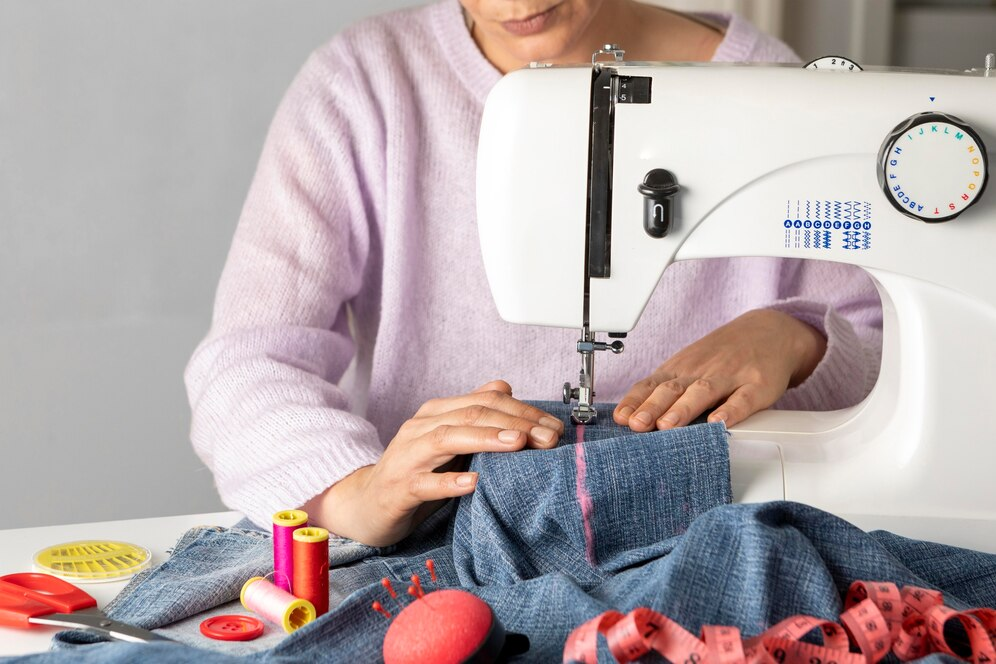
\includegraphics[width=.5\textwidth]{./imgs/img54.png}

Muitas vezes não temos ideia de que objetos tão simples que utilizamos em
nosso cotidiano chegaram até nós através de uma rede muito grande de
pessoas depois de terem sido produzidos, transportados, embalados e vendidos por
dezenas de trabalhadores.

Neste módulo vamos estudar esses diversos tipos de trabalho e entender
como eles são importantes para o nosso dia a dia.}

\pagebreak
\colorsec{Atividades}

Observe as imagens para responder às questões de 1 a 3.

\begin{figure}[htpb!]
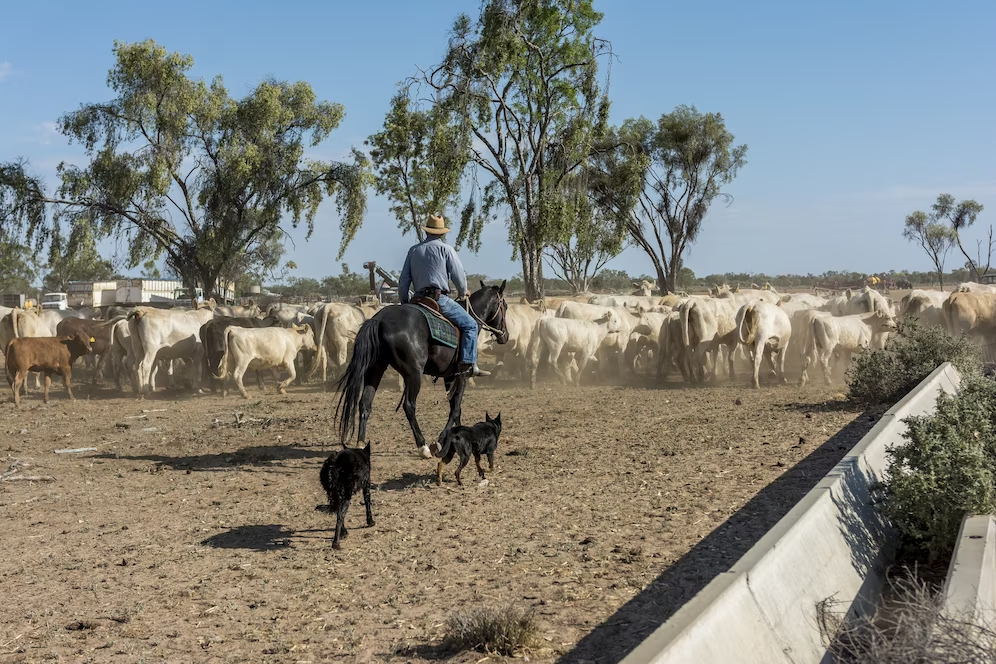
\includegraphics[width=.5\textwidth]{./imgs/img55.png}
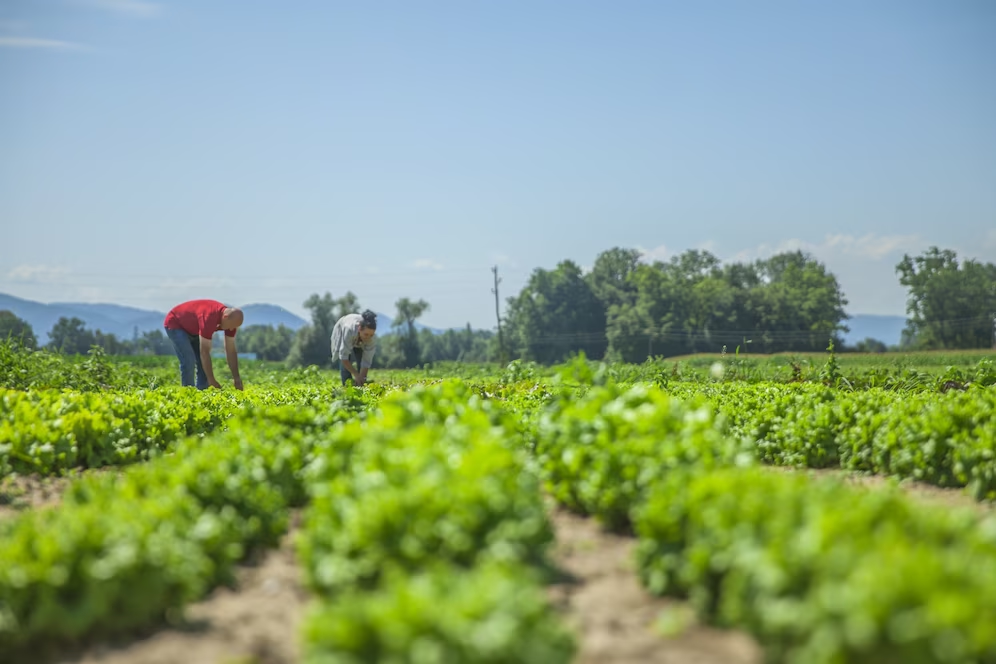
\includegraphics[width=.5\textwidth]{./imgs/img56.png}
\caption{}
\end{figure}
%\fonte{Disponível em: \emph{https://br.freepik.com/fotos-gratis/cavaleiro-liderando-um-rebanho-de-animais-em-uma-fazenda-na-australia\_9990935.htm\#query=pecu\%C3\%A1ria\&position=12\&from\_view=search\&track=sph} Acesso em 22 fev. 2023.}

%\fonte{Disponível em: \emph{https://br.freepik.com/fotos-gratis/tantos-vegetais-neste-campo\_10729697.htm\#query=agricultura\&position=8\&from\_view=search\&track=sph} Acesso em: 22 fev. 2023}

\num{1} Você reconhece algum desses lugares? Você já visitou ou viu pessoalmente algo parecido?

\reduline{Espera-se que o aluno tente reconhecer, em sua cidade ou bairro, uma
paisagem parecida com esta para, assim, entender o que se passa com os
trabalhadores que atuam naquele local e o que eles representam para sua
comunidade.\hfill}
\linhas{1}

\num{2} Com a ajuda de seu professor, preencha a tabela com características
sobre cada uma das imagens.\bigskip

\begin{tabular}{l|l}
\hline
\textbf{Imagem 1} & \textbf{Imagem 2} \\ \hline
\begin{tabular}[c]{@{}l@{}}Nome da atividade:\\ \rosa{Pecuária}\end{tabular} & \begin{tabular}[c]{@{}l@{}}Nome da atividade:\\ \rosa{Agricultura}\end{tabular} \\ \hline
Local: \rosa{Campo} & Local: \rosa{Campo} \\ \hline
\begin{tabular}[c]{@{}l@{}}Principal produto do trabalho:\\ \rosa{Alimentos de origem animal}\end{tabular} & \begin{tabular}[c]{@{}l@{}}Principal produto do trabalho:\\ \rosa{Alimentos de origem vegetal}\end{tabular} \\ \hline
\end{tabular}
\bigskip

\num{3} Agora, associe com uma seta os tipos de produto com o trabalho presente em cada uma das imagens:

\begin{multicols}{2}

Imagem 1

Imagem 2

\columnbreak

Leite

Arroz

Carne bovina

Alface
\end{multicols}

\coment{Resposta: Leite e carne bovina devem estar ligados à Imagem 1; 
Arroz e Alface, à Imagem 2}

\noindent{}Agora, vamos falar sobre Agricultura. Observe as duas imagens e, então, responda às questões que seguem.

\begin{figure}[htpb!]
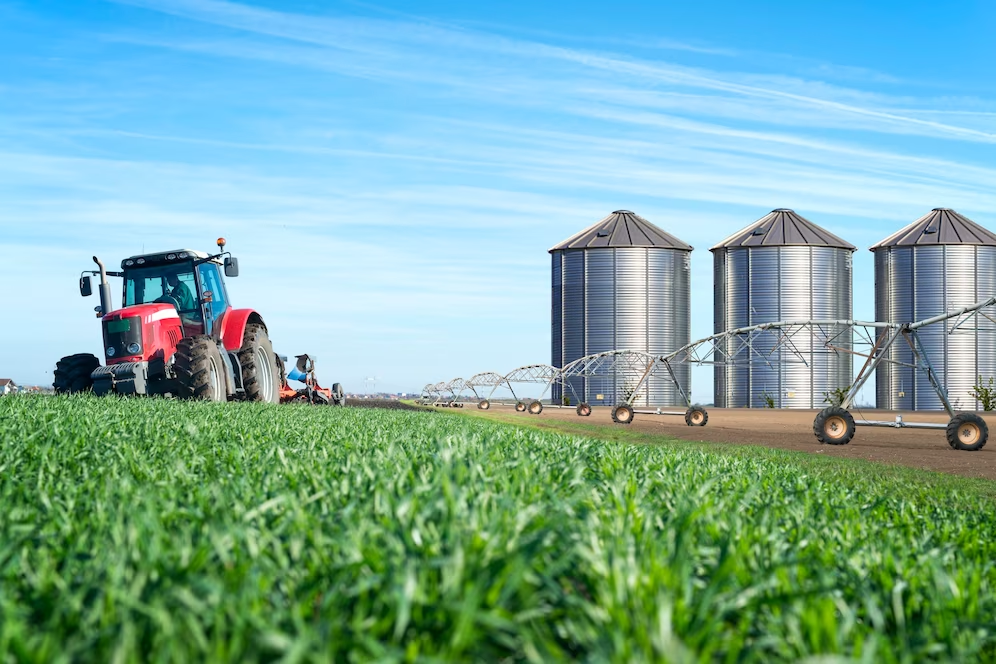
\includegraphics[width=.5\textwidth]{./imgs/img57.png}
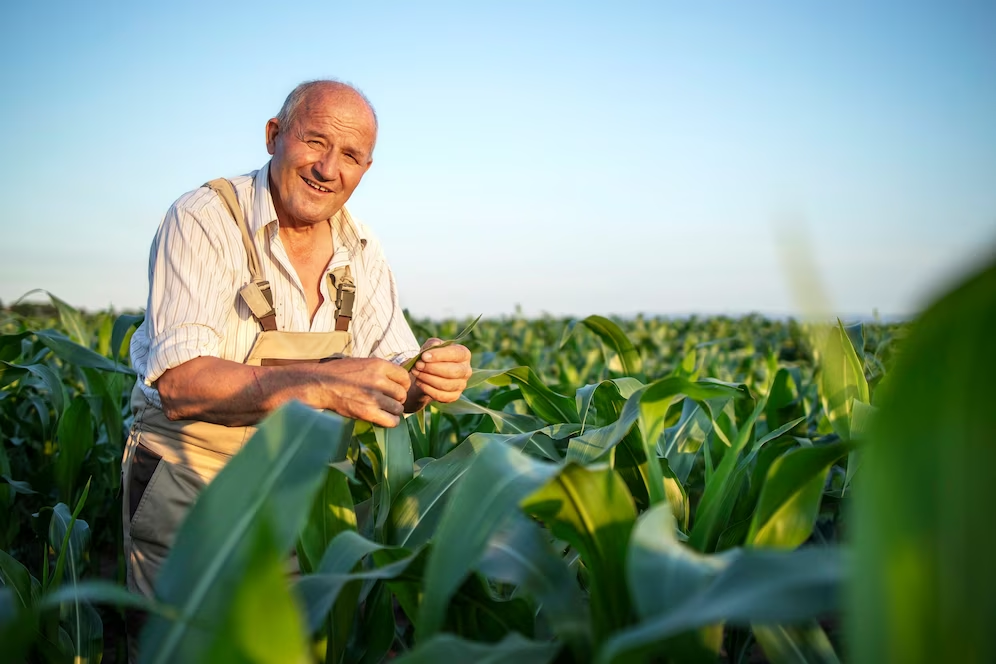
\includegraphics[width=.5\textwidth]{./imgs/img58.png}
\caption{}
\end{figure}
%Imagem 1. Disponível em: \emph{https://br.freepik.com/fotos-gratis/agricultura-e-conceito-de-producao-de-alimentos-com-silos-de-maquina-de-trator-e-sistema-de-irrigacao\_11133942.htm\#query=agricultura\&position=24\&from\_view=search\&track=sph} Acesso em: 22 fev. 2023.

%Imagem 2. Disponível em: \emph{https://br.freepik.com/fotos-gratis/retrato-de-agricultor-agronomo-senior-trabalhador-em-um-campo-de-milho-verificando-as-colheitas-antes-da-colheita\_11450848.htm\#query=agricultura\&position=35\&from\_view=search\&track=sph} Acesso em: 22 fev. 2023.

\num{4} O que você observa de semelhante entre as duas imagens?

\reduline{Ambas retratam cenas da produção agrícola.\hfill}
\linhas{1}

\num{5} Agora, registre observações do que há de diferente entre essas imagens.

\reduline{Em uma, o trator faz o trabalho; na outra, o trabalhador atua
diretamente com a colheita.\hfill}
\linhas{3}

\num{6} O que você acha que muda de uma forma de agricultura para a outra de
maneira positiva? Anote as informações passadas pelo professor. 


\reduline{Aqui, fale sobre a influência que as novas tecnologias tiveram para o
desenvolvimento da agricultura. Fale sobre a maior produtividade e
maior oferta de alimentos à população.\hfill}
\linhas{1}

\num{7} Você acha que o uso de novas tecnologias na agricultura pode ser ruim de
algum jeito? No que ele impacta na vida dos trabalhadores?

\reduline{Fale sobre a diminuição da oferta de emprego nos campos, uma vez que as
máquinas tomam o lugar dos trabalhadores. Fale sobre os movimentos de
migração do campo em busca de empregos na cidade.\hfill}
\linhas{3}

Veja, agora, alguns dados sobre o processo de modernização na agricultura.

\begin{quote}
Com a “modernização conservadora” ocorreu uma diminuição significativa
da oferta de trabalho no campo na região Centro-Oeste e principalmente
no Estado de Goiás. De acordo com o IBGE – Instituto Brasileiro de
Geografia e Estatística - entre 1985 e 1996 houve uma redução de 20\%
dos trabalhadores rurais no Centro-Oeste.

Em 1985, existiam cerca 1,5 milhão de trabalhadores no campo, e em 1996,
os trabalhadores rurais somavam aproximadamente 1,2 milhão de
trabalhadores. Em Goiás, em 1985, os trabalhadores rurais somavam
616.000.

Uma década depois (1996) existiam cerca de 472.000 trabalhadores rurais,
ocorrendo uma redução de aproximadamente 23\%, expressando as mudanças
no trabalho após a adoção das inovações técnicas.

\fonte{
Mendonça, M. R. (2011). A Modernização da Agricultura e os impactos
sobre o trabalho. {PEGADA - A Revista Da Geografia Do Trabalho,
3}. Disponível em: https://doi.org/10.33026/peg.v3i0.789. Acesso em 23 mar. 2023.}
\end{quote}

\colorsec{Atividade 3}

Agora, vamos ver como esse processo dá origem a outro: \textbf{a migração}.

\coment{BNCC EF05GE05: Identificar e comparar as mudanças dos tipos de trabalho
e desenvolvimento tecnológico na agropecuária, na indústria, no comércio
e nos serviços.

SAEB 7C1: Avaliar o papel desempenhado pela migração e seus efeitos nas
regiões de destino.

7B8: 8. Compreender as transformações nas relações entre campo e cidade
envolvendo os fluxos de trabalhadores.

7B2: Analisar diferentes fluxos populacionais e suas contribuições para
a formação da sociedade brasileira.
}

Segundo Mendonça, a modernização no campo “historicamente promoveu a
migração forçada dos trabalhadores (pequenos produtores rurais)
resultando em expropriação fundiária que `esvazia o campo e urbaniza a
sociedade'.” Ou seja, a falta de empregos no campo levou os
trabalhadores a irem para a cidade em busca de novas oportunidades de
trabalho.

\fonte{Mendonça, M. R. (2011). A Modernização da Agricultura e os impactos
sobre o trabalho. \textbf{PEGADA - A Revista Da Geografia Do Trabalho,
3}. Disponível em: \emph{https://doi.org/10.33026/peg.v3i0.789}. Acesso em 23 mar. 2023.}

\num{8} Você sabe o que é \textbf{migração}? Descreva a seguir com a ajuda de seu professor.

\reduline{Definir migração para o aluno: movimentação de entrada (imigração) ou
saída (emigração) de indivíduo ou grupo de indivíduos, em busca de
melhores condições de vida. Explique, ainda, que essa movimentação pode se dar entre países
diferentes ou dentro de um mesmo país.\hfill}
\linhas{3}

\num{9} Você conhece alguém que já migrou? Qual foi o motivo? Converse com seus
colegas sobre isso.

\coment{Aqui o aluno deve relembrar suas próprias experiências. É comum que
alguém da família tenha vindo de algum lugar, mudado de cidade ou estado
por motivos familiares, financeiros, entre outros. Deixe que os alunos
conversem e compartilhem suas experiências.}

\num{10} Observe a imagem e responda às questões propostas.

\begin{figure}[htpb!]
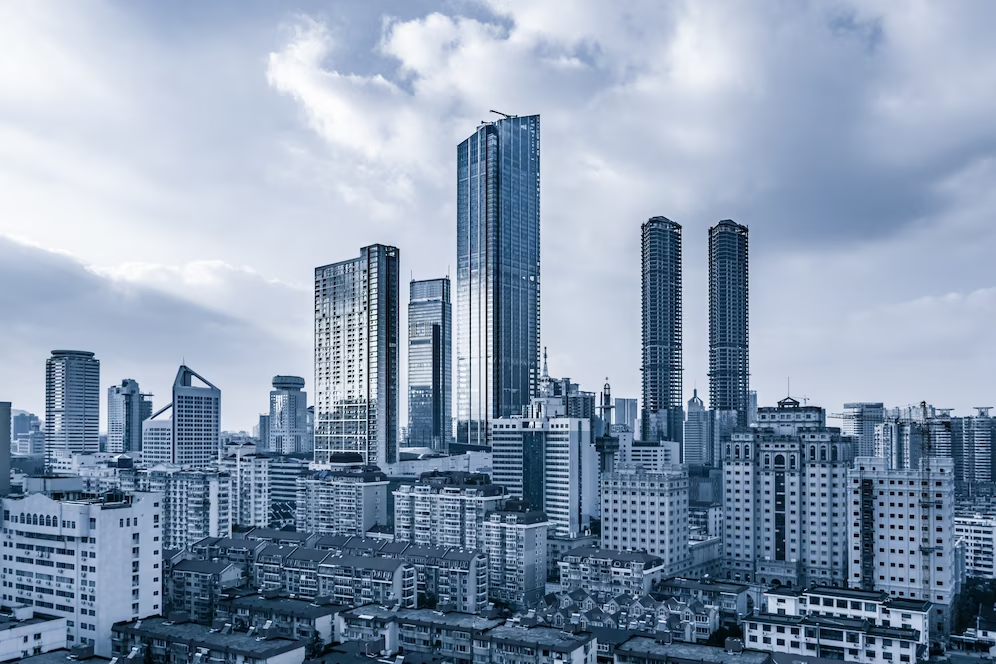
\includegraphics[width=.5\textwidth]{./imgs/img59.png}
%\caption{Disponível em: \emph{https://br.freepik.com/fotos-gratis/steel-business-predio-urbano-observacao\_1046153.htm\#query=S\%C3\%A3o\%20Paulo\&position=2\&from\_view=search\&track=ais} Acesso em: 23 fev. 2023.}
\end{figure}

\noindent{}O que você acha que pode acontecer se muitas pessoas migram para um mesmo lugar (uma cidade, por exemplo) muito rapidamente?

\reduline{Fale com os alunos sobre as consequências de uma migração forçada, no
caso dos trabalhadores rurais que perderam seus empregos por causa da
tecnologia. Fale sobre como o crescimento desordenado das cidades pode
afetar na vida das pessoas que moram lá e trazer graves
consequências de precarização na saúde, na moradia e no trabalho.\hfill}
\linhas{2}

\num{11} Observe as imagens.

\begin{figure}[htpb!]
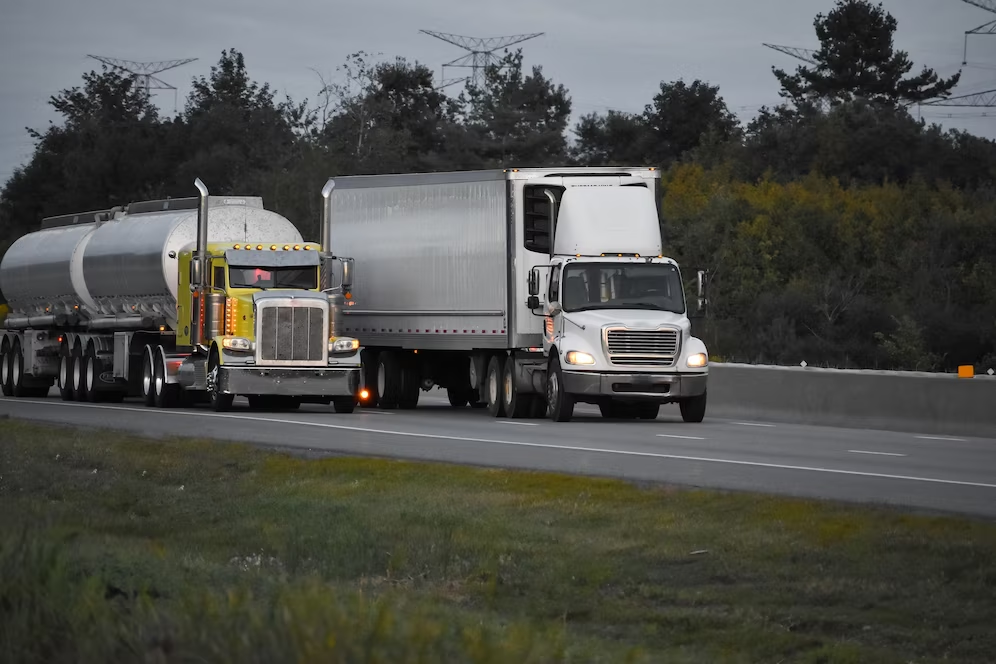
\includegraphics[width=.5\textwidth]{./imgs/img60.png}
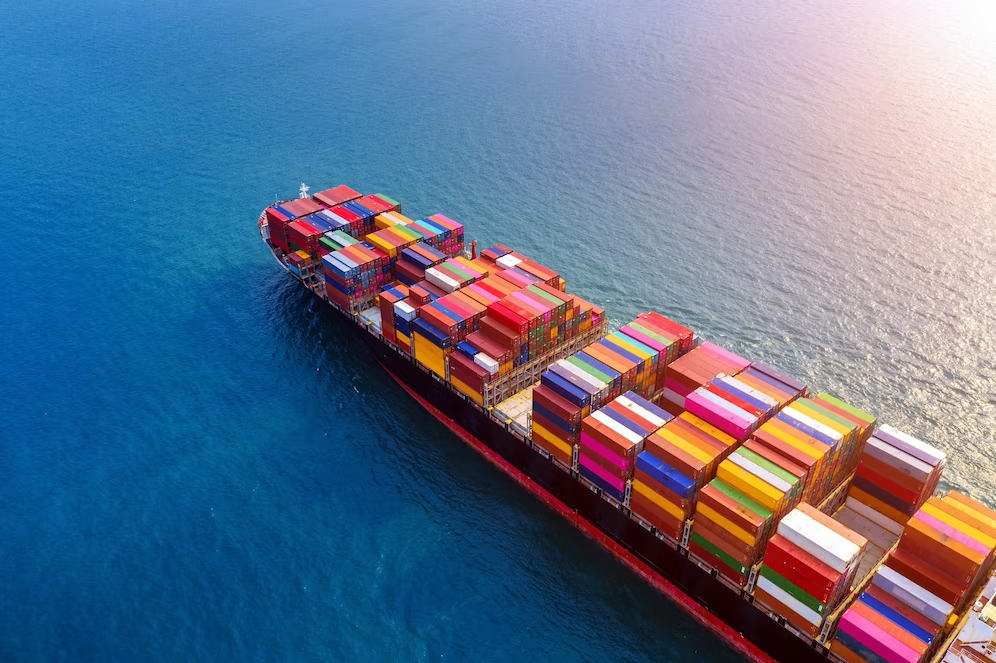
\includegraphics[width=.5\textwidth]{./imgs/img61.png}
\end{figure}


\begin{figure}[htpb!]
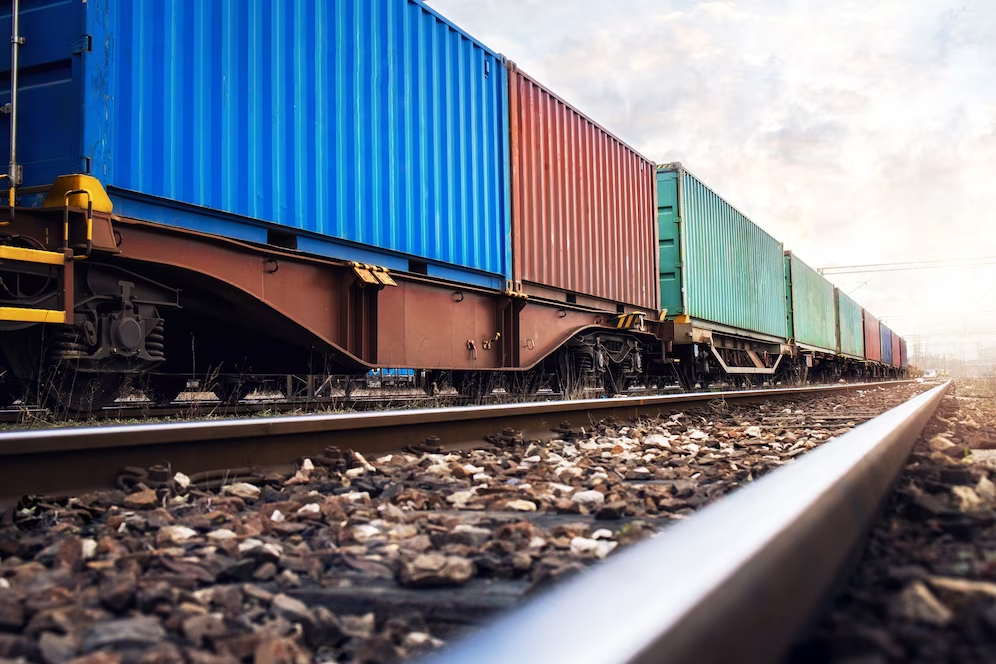
\includegraphics[width=.5\textwidth]{./imgs/img62.png}
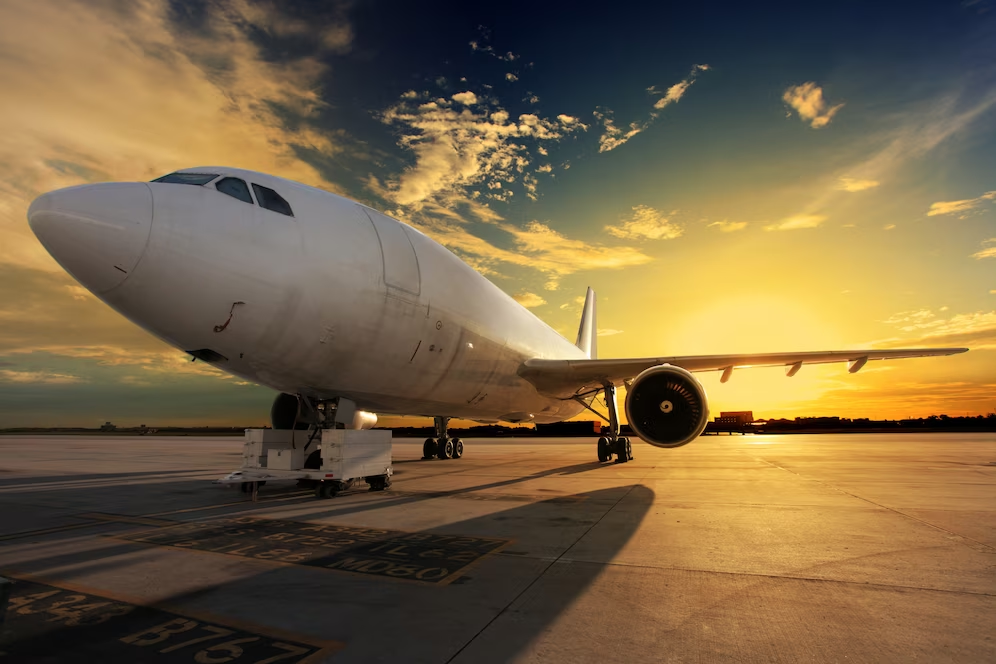
\includegraphics[width=.5\textwidth]{./imgs/img63.png}
\end{figure}

%1)Caminhão: \emph{https://br.freepik.com/fotos-gratis/caminhoes-de-reboque-dirigindo-na-estrada-cercados-por-belas-arvores-verdes\_9932046.htm\#query=caminh\%C3\%A3o\&position=6\&from\_view=search\&track=sph}

%2)Barco: \emph{https://br.freepik.com/fotos-gratis/vista-aerea-do-navio-de-carga-do-conteiner-no-mar\_13180387.htm\#query=barco\%20carga\&position=0\&from\_view=search\&track=ais}

%3)Trem: \emph{https://br.freepik.com/fotos-gratis/vagoes-de-trem-transportando-conteineres-de-carga-para-empresas-de-navegacao\_11136398.htm\#query=ferrovia\&position=1\&from\_view=search\&track=sph}

%4)Avião: \emph{https://br.freepik.com/fotos-gratis/aviao-ao-por-do-sol\_4291511.htm\#query=avi\%C3\%A3o\&position=11\&from\_view=search\&track=sph}

As quatro imagens representam quatro vias de transportes que utilizamos
para a \textbf{circulação de mercadorias} no Brasil. Você sabe o nome
delas? Com a ajuda de seu professor, complete na ordem das imagens.
Colocar quatro linhas numeradas.

\begin{enumerate}
\item \reduline{Rodovia (estradas)\hfill}

\item \reduline{Hidrovia (rios e mares)\hfill}

\item \reduline{Ferrovia (Trens e locomotivas)\hfill}

\item \reduline{Aerovia (Aviões)\hfill}

\end{enumerate}

\num{12} Para comandar cada um desses transportes, existem pessoas, trabalhadores que participam do processo. Vamos ler um
pouco sobre o trabalho de um caminhoneiro nesta reportagem sobre o Dia
do Caminhoneiro.

\begin{quote}
\textbf{Dia do Caminhoneiro: motoristas falam sobre os desafios de
exercer a profissão}

São horas atrás do volante, dias fora de casa e metas a cumprir. Saudade
da família e os perigos nas estradas fazem parte da rotina diária dos
motoristas de cargas. {[}\ldots{}{]}

Casado, pai de um menino de 15 anos e de uma menina de 1 ano e 6 meses,
Costa disse que conversa com a família todos os dias. “Quando eu comecei
a trabalhar, meu menino já era grandinho e às vezes ele ia comigo nas
viagens mais curtas. Agora com a pequenininha ficou mais dolorido ficar
fora de casa”, afirmou ele. {[}\ldots{}{]}

“Para você estar usando seu celular hoje, chegou até você por um
caminhão. Seu carro não anda se você não tiver combustível, que chega
até o posto por meio de um caminhão. O café da manhã, aquele leite,
aquela farinha que fez o pão, tudo passou por um caminhão”, disse. {[}\ldots{}{]}

\fonte{ Kalinka Bacacicci. G1. Dia do Caminhoneiro: motoristas falam sobre os desafios de exercer a profissão. Disponível em:
\emph{https://g1.globo.com/sp/sao-carlos-regiao/noticia/dia-do-caminhoneiro-motoristas-falam-sobre-os-desafios-de-exercer-a-profissao.ghtml}.
Acesso em: 23 fev. 2023.}
\end{quote}

\pagebreak
\num{a} Segundo o texto, qual é a importância do trabalho de pessoas como Costa?

\reduline{A partir de seu trabalho chega até nós tudo a que temos acesso em nosso
dia a dia, como comida, roupas, objetos da casa etc.\hfill}
\linhas{2}

\num{b} Com a ajuda de seus colegas, faça uma lista de outras profissões que
você acha que também são importantes no processo de circulação de
mercadorias até chegar à nossa casa.

\begin{enumerate}
\item \reduline{\hfill}

\item \reduline{\hfill}

\item \reduline{\hfill}

\item \reduline{\hfill}

\item \reduline{\hfill}

\item \reduline{\hfill}

\item \reduline{\hfill}

\item \reduline{\hfill}
\end{enumerate}

\coment{Nesse momento, deixe que os alunos conversem entre si para chegar às
profissões. Você pode anotar na lousa as profissões que forem surgindo
ao longo do debate.}

\pagebreak
\colorsec{Treino}

\num{1}

\begin{figure}[htpb!]
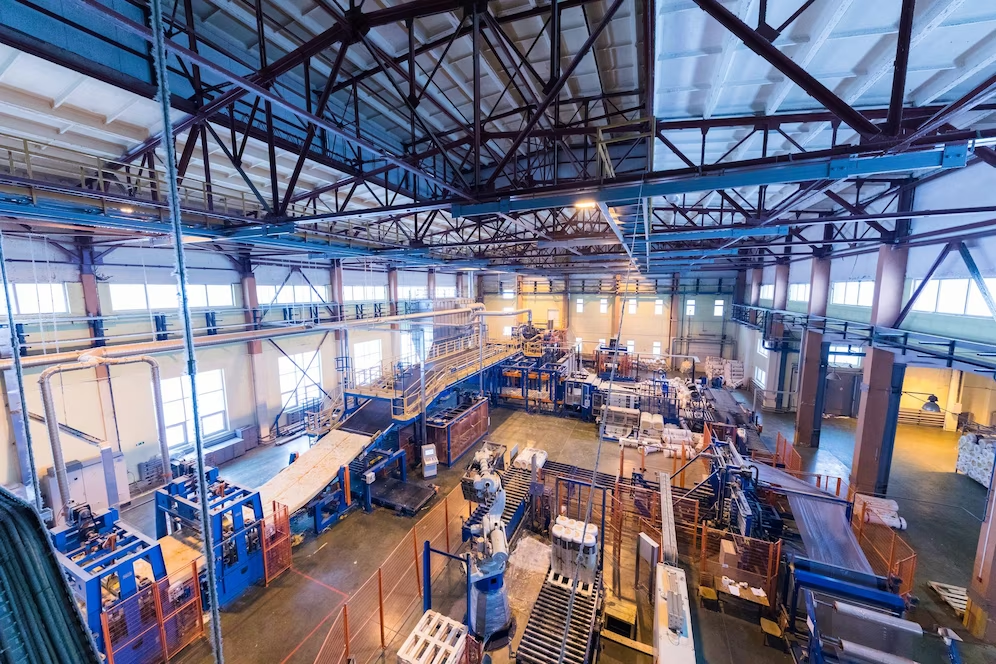
\includegraphics[width=.5\textwidth]{./imgs/img64.png}
%\caption{Disponível em: \emph{https://br.freepik.com/fotos-gratis/interior-de-oficina-de-fabrica-e-maquinas-em-fundo-de-producao-de-vidro\_26150555.htm\#query=ind\%C3\%BAstria\&position=26\&from\_view=search\&track=sph} Acesso em: 23 fev. 2023}
\end{figure}

A imagem acima representa a seguinte forma de trabalho:

\begin{minipage}{0.5\textwidth}
\begin{escolha}
\item Pecuária.

\item Produção agrícola.

\item Produção industrial.

\item Extrativismo mineral.
\end{escolha}
\end{minipage}
\sidetext{BNCC: EF05GE05 - Identificar e comparar as mudanças dos tipos de trabalho
e desenvolvimento tecnológico na agropecuária, na indústria, no comércio
e nos serviços.}


\num{2} As metrópoles do século 21 mesclam trens, automóveis, ônibus e bondes
com o resgate de opções antigas e mais sustentáveis, como a bicicleta.
Contudo, ao longo da história, pessoas e cargas já foram movimentadas
por veículos bem diferentes dos que conhecemos hoje: meios de transporte
antigos que não são mais usados em larga escala acabaram virando peça de
museu ou objeto de curiosidade. {[}\ldots{}{]}

\fonte{Estadão. Meios de transporte antigos: 4 modais que não existem mais. Disponível em:
\emph{https://summitmobilidade.estadao.com.br/ir-e-vir-no-mundo/meios-de-transporte-antigos-4-modais-que-nao-existem-mais/}.
Acesso em: 23 fev. 2022}

Um exemplo de transporte antigo usado para o deslocamento de mercadorias é

\begin{minipage}{0.5\textwidth}
\begin{escolha}
\item o avião de carga.

\item a carruagem puxada por cavalo.

\item o caminhão carreta.

\item a moto de delivery.
\end{escolha}
\end{minipage}
\sidetext{BNCC: EF05GE05 - Identificar e comparar as mudanças dos tipos de trabalho
e desenvolvimento tecnológico na agropecuária, na indústria, no comércio
e nos serviços.}


\num{3} A história da descoberta do vidro é bem antiga e os primeiros
registros datam de 5000 a.C. {[}\ldots{}{]} Em 1952, foi revelada uma invenção que
mudou tudo. Fazendo flutuar vidro derretido em estanho também derretido,
Pilkington conseguiu produzir vidro quase tão plano quanto suas placas
prensadas e polidas, a uma espessura econômica e em grandes quantidades,
através de um processo contínuo. {[}\ldots{}{]} Essa única invenção revolucionou e
petrificou a indústria. {[}\ldots{}{]}

\fonte{ Vidrado. História da produção do vidro. Disponível em: \emph{https://vidrado.com/noticias/historia/historia-da-producao-do-vidro/}. Acesso em: 23 fev. 2023.}

O texto fala sobre a

\begin{escolha}
\item falta de estudos técnicos sobre materiais descobertos na antiguidade.

\item necessidade de manter técnicas tradicionais na produção em massa.

\item importância de novas tecnologias para o desenvolvimento industrial.

\item dificuldade de viver em sociedades antigas que não tinham indústrias.
\end{escolha}

\coment{BNCC: EF05GE05 - Identificar e comparar as mudanças dos tipos de trabalho
e desenvolvimento tecnológico na agropecuária, na indústria, no comércio
e nos serviços.}



